%%%%%%%%%%%%%%%%%%%%%%%%%%%%%%%%%%%%%%%%%%%%%%%%%%%%%%%%%%%%%%%%%%%%%%%%
%%                                                                    %%
%% This is file `ucalgarythesis.tex'  -- a document template for      %%
%% graduate theses at the University of Calgary.                      %%
%%                                                                    %%
%% This template document is to be used in conjunction with the       %%
%% thesis class file `ucalgarythesis.cls'.                            %%
%%                                                                    %%
%% Created by M.W. Girard, last updated 10 April 2016.                %%
%%                                                                    %%
%% This template was created to be in compliance with the University  %%
%% of Calgary thesis guidelines (version 14 April 2014)               %%
%%       https://grad.ucalgary.ca/current/thesis/guidelines.          %%
%%                                                                    %%
%%%%%%%%%%%%%%%%%%%%%%%%%%%%%%%%%%%%%%%%%%%%%%%%%%%%%%%%%%%%%%%%%%%%%%%%
%%                                                                    %%
%% By default, the text of the thesis is doublespaced and should be   %%
%% printed single-sided. All margins must be exactly one inch on all  %%
%% sides, and should not be bound or have binding edges. This is      %%
%% required by the University of Calgary thesis guidelines.           %%
%% All theses are now required to be submitted electronically.        %%
%%                                                                    %%
%%%%%%%%%%%%%%%%%%%%%%%%%%%%%%%%%%%%%%%%%%%%%%%%%%%%%%%%%%%%%%%%%%%%%%%%


%%%%%%%%%%%%%%%%%%%%%%%%%%%%%%%%%%%%%%%%%%%%%%%%%%%%%%%%%%%%
%%
%% Load the `ucalgarythesis.cls' document class
%%%%%%%%%%%%%%%%%%%%%%%%%%%%%%%%%%%%%%%%%%%%%%%%%%%%%%%%%%%%

\documentclass{ucalgarythesis}

%%%%%%%%%%%%%%%%%%%%%%%%%%%%%%%%%%%%%%%%%%%%%%%%%%%%%%%%%%%%%%%%%%%%%%
%% If you would like to print a personal copy of your thesis for    %%
%% your own record, you may print it double-sided and with extra    %%
%% margins for binding. Use the following line instead of the above %%
%% \documentclass{ucalgarythesis} for compiling personal copies of  %%
%% the thesis to be printed double-sided and bound.                 %%
%%%%%%%%%%%%%%%%%%%%%%%%%%%%%%%%%%%%%%%%%%%%%%%%%%%%%%%%%%%%%%%%%%%%%%
%\documentclass[twoside,binding]{ucalgarythesis}

%%%%%%%%%%%%%%%%%%%%%%%%%%%%%%%%%%%%%%%%%%%%%%%%%%%%%%%%%%%%
%%
%% Imported packages & custom user commands
%%%%%%%%%%%%%%%%%%%%%%%%%%%%%%%%%%%%%%%%%%%%%%%%%%%%%%%%%%%%

%% Include extra packages here

\usepackage[utf8]{inputenc}
\usepackage{amssymb,amsmath,amsthm}
%\usepackage[hidelinks]{hyperref}
\usepackage{algorithm}
%\usepackage{algorithmic}
\usepackage{algpseudocode}
\usepackage{comment}
\usepackage{enumitem}
\usepackage{graphicx}
\usepackage{multirow}
\usepackage{hyperref}
\usepackage{pgfplots}
\usepackage{tabularx}
\usepackage{tikz-cd}
\usepackage[style=numeric, backend=biber]{biblatex}
\bibliography{biblio}
%\bibliographystyle{plain}

%\usepackage{biblatex}

\hypersetup{
    colorlinks,
    citecolor=blue,
    filecolor=blue,
    linkcolor=blue,
    urlcolor=blue
}

%%  Include other user-defined commands here

\let\div\undefined
\renewcommand{\bar}{\overline}

\newlength{\tempabovedisplayskip}
\newlength{\tempbelowdisplayskip}
\algnewcommand{\algorithmicgoto}{\textbf{go to}}
\algnewcommand{\GoTo}[1]{\algorithmicgoto~{#1}}

\DeclareMathOperator{\Char}{char}
\DeclareMathOperator{\Cl}{Cl}
\DeclareMathOperator{\coeff}{coeff}
\DeclareMathOperator{\coim}{coim}
\DeclareMathOperator{\coker}{coker}
\DeclareMathOperator{\Der}{Der}
\DeclareMathOperator{\Div}{Div}
\DeclareMathOperator{\div}{div}
\DeclareMathOperator{\Frac}{Frac}
\DeclareMathOperator{\Gal}{Gal}
\DeclareMathOperator{\Hom}{Hom}
\DeclareMathOperator{\Id}{Id}
\DeclareMathOperator{\im}{im}
\DeclareMathOperator{\lcm}{lcm}
\DeclareMathOperator{\Jac}{Jac}
\DeclareMathOperator{\LM}{LM}
\DeclareMathOperator{\LT}{LT}
\DeclareMathOperator{\Ker}{Ker}
\DeclareMathOperator{\nullity}{null}
\DeclareMathOperator{\Pic}{Pic}
\DeclareMathOperator{\Princ}{Princ}
\DeclareMathOperator{\RGB}{RGB}
\DeclareMathOperator{\rref}{RREF}
\DeclareMathOperator{\orb}{orb}
\DeclareMathOperator{\ord}{ord}
\DeclareMathOperator{\rank}{rank}
\DeclareMathOperator{\supp}{supp}
\DeclareMathOperator{\Span}{Span}
\DeclareMathOperator{\type}{type}
%\DeclareMathOperator{\KVec}{K-Vec}

\newcommand{\inv}{^{-1}}
\newcommand{\pid}[1]{\left\langle #1 \right\rangle}

%\newcommand{\der}{\partial}
\newcommand{\defn}{\textbf}
\newcommand{\note}[1]{{\color{red}#1}}
\newcommand{\bb}[1]{\mathbb{#1}}
\newcommand{\tensor}[1]{\underset{#1}{\otimes}}
\renewcommand{\cal}[1]{\mathcal{#1}}

\numberwithin{equation}{section}
\numberwithin{figure}{section}
\numberwithin{table}{section}
\numberwithin{algorithm}{section}

\theoremstyle{plain}
\newtheorem{theorem}[equation]{Theorem}
\newtheorem{corollary}[equation]{Corollary}
\newtheorem{conjecture}[equation]{Conjecture}
\newtheorem{lemma}[equation]{Lemma}
\newtheorem{proposition}[equation]{Proposition}

\theoremstyle{definition}
\newtheorem{definition}[equation]{Definition}
\newtheorem{example}[equation]{Example}
\newtheorem{remark}[equation]{Remark}

\renewcommand*{\arraystretch}{0.8} % Adjust spacing between lines in matrices

\renewcommand\thesection{\arabic{section}} % Fix section/subsection numbering style
\renewcommand\thesubsection{\thesection.\arabic{subsection}}

%%%%%%%%%%%%%%%%%%%%%%%%%%%%%%%%%%%%%%%%%%%%%%%%%%%%%%%%%%%%%%%%%%%%%%%%
%%                                                                    %%
%% Begin document                                                     %%
%%                                                                    %%
%%%%%%%%%%%%%%%%%%%%%%%%%%%%%%%%%%%%%%%%%%%%%%%%%%%%%%%%%%%%%%%%%%%%%%%%
\begin{document}

%%%%%%%%%%%%%%%%%%%%%%%%%%%%%%%%%%%%%%%%%%%%%%%%%%%%%%%%%%%%%%%%%%%%%%%%
%%                                                                    %%
%% Title page                                                         %%
%%                                                                    %%
%%%%%%%%%%%%%%%%%%%%%%%%%%%%%%%%%%%%%%%%%%%%%%%%%%%%%%%%%%%%%%%%%%%%%%%%

%%%%%%%%%%%%%%%%%%%%%%%%%%%%%%%%%%%%%%%%%%%%%%%%%%%%%%%%%%%%%%%%%%%%%%%%
%% Instructions for title page information:                           %%
%%                                                                    %%
%%  Fill in the following fields with the required information:       %%
%%   - \title{...}        Title of the thesis                         %%
%%   - \author{...}       Your full name                              %%
%%   - \thesis{Thesis}    Type of document (may change to `Thesis' to %%
%%                           `Dissertation' depending on type of work)%%
%%   - \dept{...}         Full name of the graduate department or     %%
%%                           degree program                           %%
%%   - \degree{...}       Full name of the degree obtained            %%
%%                          (i.e. Doctor of Philosophy,               %%
%%                                 Master of Science, etc)            %%
%%   - \gradyear{...}     Year of submission                          %%
%%   - \monthname{...}    Month of submission                         %%
%%%%%%%%%%%%%%%%%%%%%%%%%%%%%%%%%%%%%%%%%%%%%%%%%%%%%%%%%%%%%%%%%%%%%%%%

\title{Divisor Class Group Arithmetic on $C_{3,4}$ Curves}
 
\author{Evan MacNeil}
\thesis{Thesis}
\dept{Graduate Program in Mathematics and Statistics}
\degree{Master of Science}
\gradyear{2019}
\monthname{August}


%%%%%%%%%%%%%%%%%%%%%%%%%%%%%%%%%%%%%%%%%%%%%%%%%%%  
%% Make the thesis title page.
%%%%%%%%%%%%%%%%%%%%%%%%%%%%%%%%%%%%%%%%%%%%%%%%%%%
\frontmatter           %% Don't remove this line.
\makethesistitle       %% Don't remove this line.


%%%%%%%%%%%%%%%%%%%%%%%%%%%%%%%%%%%%%%%%%%%%%%%%%%%%%%%%%%%%%%%%%%%%%%%%
%%                                                                    %%
%% Prefatory pages                                                    %%
%%                                                                    %%
%%%%%%%%%%%%%%%%%%%%%%%%%%%%%%%%%%%%%%%%%%%%%%%%%%%%%%%%%%%%%%%%%%%%%%%%
%% The following sections are in the correct order as specified by    %%
%% the April 2014 thesis guidelines set by the University of Calgary. %%
%%                                                                    %%
%% You may remove optional sections, but do not change the order.     %%
%%%%%%%%%%%%%%%%%%%%%%%%%%%%%%%%%%%%%%%%%%%%%%%%%%%%%%%%%%%%%%%%%%%%%%%%

%%%%%%%%%%%%%%%%%%%%%%%%%%%%%%%%%%%%%%%%%%%%%%%%%%%
%%
%% Abstract page (REQUIRED)
%%%%%%%%%%%%%%%%%%%%%%%%%%%%%%%%%%%%%%%%%%%%%%%%%%%

\begin{thesisabstract}  

Computing in the divisor class group of an algebraic curve is a non-trivial component in computing $L$-series.
$L$-series in turn are at the heart of the Sato-Tate conjecture and related conjectures.
The Sato-Tate conjecture has been proven for elliptic curves with complex multiplication,
but remains open for other families of algebraic curves.
In order to test these conjectures against other curve families, it is desirable to have efficient algorithms to perform divisor class group arithmetic.

Fast explicit formulas exist to perform divisor class group arithmetic for genus 1 and genus 2 curves.
However, the picture for genus 3 curves is incomplete.
Existing explicit formulas for arithmetic on non-hyperelliptic genus 3 curves ($C_{3,4}$ curves) have been developed with cryptographic applications in mind.
They make certain generacity assumptions on their inputs that hold with high probability in cryptographic settings,
but are unsuited for number theoretic use cases.
More general algorithms exist that can perform divisor class arithmetic over any curve, but they are slow.
The goal of this project is to bridge the gap --
to find fast explicit formulas describing $C_{3,4}$ curve arithmetic that are correct for all inputs.

\end{thesisabstract}


%%%%%%%%%%%%%%%%%%%%%%%%%%%%%%%%%%%%%%%%%%%%%%%%%%%
%%
%% Preface page (OPTIONAL)
%%%%%%%%%%%%%%%%%%%%%%%%%%%%%%%%%%%%%%%%%%%%%%%%%%%

%% This section is required if the work presented in the thesis is 
%% done as part of a collaboration. In this case, the preface must 
%% state which part of the thesis are the author's original work.
%% Otherwise this section is optional.

  \chapter{Preface}
 
  This thesis is an original work by the author. No part of this thesis has been previously published.
 
  % Some of the research conducted for this thesis forms part of an international research collaboration, led by Professor R.C. Smith at the University of Hogwarts
   
 
%%%%%%%%%%%%%%%%%%%%%%%%%%%%%%%%%%%%%%%%%%%%%%%%%%%
%%
%% Acknowledgements page (REQUIRED)
%%%%%%%%%%%%%%%%%%%%%%%%%%%%%%%%%%%%%%%%%%%%%%%%%%%

  \chapter{Acknowledgements}  
  
Thank you to my family.
Your thoughts, prayers, and support were felt 4,500 km away.

Thank you to my supervisors, Dr. Renate Scheidler and Dr. Michael Jacobson.
Your expertise in class group computations helped me get this project started.
Your expertise in time management helped me finish.

Thank you to my fellow graduate students and officemates.
Randy Yee, who poked holes in my proofs like a mathematical awl.
Without you, the proofs in this thesis would look awfully stupid.
Sumin Leem, who was always happy to help.
Your experience with function fields was invaluable to my early understanding of curves.
Geoff Vooys, who always had a different perspective on a problem and three references.
When I was stuck on something, your take always led somewhere fruitful.


    
%%%%%%%%%%%%%%%%%%%%%%%%%%%%%%%%%%%%%%%%%%%%%%%%%%
%%
%% Dedication page (this section is OPTIONAL)
%%%%%%%%%%%%%%%%%%%%%%%%%%%%%%%%%%%%%%%%%%%%%%%%%%

%  \chapter[Dedication]{}
%  
%  \begin{dedication}
%     \emph{To all the time I've wasted...}
%  \end{dedication}

%%%%%%%%%%%%%%%%%%%%%%%%%%%%%%%%%%%%%%%%%%%%%%%%%%
%%
%% Various lists
%%%%%%%%%%%%%%%%%%%%%%%%%%%%%%%%%%%%%%%%%%%%%%%%%%
%% The Table of Contents and all Lists should be single spaced.

  \begin{singlespace}   %% Do not remove this line

%%%%%%%%%%%%%%%%%%%%%%%%%%%%%%%%%%%%%%%%%%%%%%%%%%
%%
%% Table of Contents (REQUIRED)
%%%%%%%%%%%%%%%%%%%%%%%%%%%%%%%%%%%%%%%%%%%%%%%%%%
  \renewcommand\contentsname{Table of Contents}
  \cleardoublepage\phantomsection
  \addcontentsline{toc}{chapter}{\contentsname}
  \tableofcontents

%%%%%%%%%%%%%%%%%%%%%%%%%%%%%%%%%%%%%%%%%%%%%%%%%%
%% List of figures (required, if any)
  \renewcommand{\listfigurename}{List of Figures and Illustrations}
  \cleardoublepage\phantomsection
  \addcontentsline{toc}{chapter}{\listfigurename}
  \listoffigures

%%%%%%%%%%%%%%%%%%%%%%%%%%%%%%%%%%%%%%%%%%%%%%%%%%
%% List of tables (required, if any)
  \renewcommand{\listtablename}{List of Tables}
  \cleardoublepage\phantomsection
  \addcontentsline{toc}{chapter}{\listtablename}
  \listoftables
  
%%%%%%%%%%%%%%%%%%%%%%%%%%%%%%%%%%%%%%%%%%%%%%%%%%
%% List of Symbols, abbreviations, and nomenclature (required, if any)   
%%
%% (Note: You may use your own format for your list of symbols, 
%%  abbreviations, etc. This format is just a guideline.)
%%
\begin{comment}
  \chapter{List of Symbols, Abbreviations and Nomenclature}      
  \begin{tabbing}
    Symbol or abbreviation~~~~~\= \ \ \ \ \ \ \ \ \ \ \ \ \ \ \ \ \ \ \ \ \ \ \ \ \ \ \ \ \ \ \ \ \ \ \ \  \parbox{5in}{Definition}\\

    \addsymbol \mbox{$\alpha$}: {The first letter of the Greek alphabet}
    \addsymbol \mbox{$\beta$}: {The second letter of the Greek alphabet}
    %
    % Add more symbols here...
    % . 
    % .
    % .
    %
    
    % Always keep the following line if you are using a list of symbols:
  \end{tabbing}
\end{comment}
%%%%%%%%%%%%%%%%%%%%%%%%%%%%%%%%%%%%%%%%%%%%%%%%%%
%% End single spacing after last list
  \end{singlespace}     %% Do not remove this line
  
%%%%%%%%%%%%%%%%%%%%%%%%%%%%%%%%%%%%%%%%%%%%%%%%%%
%
% Epigraph (this section is OPTIONAL)
%%%%%%%%%%%%%%%%%%%%%%%%%%%%%%%%%%%%%%%%%%%%%%%%%%

%  \chapter{Epigraph}
%  \begin{epiquote} 
%   \textit{A quotation is a handy thing to have about, saving one the trouble of thinking for oneself, always a laborious business.} 
%  \end{epiquote}    
%  \begin{flushright} - A.A. Milne, \textit{If I May}\end{flushright}\bigskip
   

%%%%%%%%%%%%%%%%%%%%%%%%%%%%%%%%%%%%%%%%%%%%%%%%%%%%%%%%%%%%%%%%%%%%%%%%
%%                                                                    %%
%% Main matter                                                        %%
%%                                                                    %%
%%%%%%%%%%%%%%%%%%%%%%%%%%%%%%%%%%%%%%%%%%%%%%%%%%%%%%%%%%%%%%%%%%%%%%%%

  \mainmatter           %% Do not remove this line
    
%%%%%%%%%%%%%%%%%%%%%%%%%%%%%%%%%%%%%%%%%%%%%%%%%%
%%
%% Chapters
%%%%%%%%%%%%%%%%%%%%%%%%%%%%%%%%%%%%%%%%%%%%%%%%%%

\setcounter{page}{10}

%%%%%%%%%%%%%%%%%%%%%%%%%%
%%%%%                %%%%%
%%%%%   Background   %%%%%
%%%%%                %%%%%
%%%%%%%%%%%%%%%%%%%%%%%%%%

\section{Background and Motivation}

$L$-series are central to many conjectures in number theory.
A complete discussion of $L$-series is outside the scope of this thesis;
we present only enough to motivate the topic of this thesis.

Let $E$ be an elliptic curve defined over the rational numbers $\bb Q$.
The $L$-series of $E$ is
\[ L(E/\bb Q, s)  = \prod_{p \text{ is prime}} \frac 1 {L_p \left( \frac 1 {p^s} \right)},\]
where, for each prime $p$, $L_p$ is a non-zero polynomial of degree at most 2.
\note{See Silverman, or Milne for more, including a definition of $L_p$.}

By Hasse's Theorem, the number of points on an elliptic curve defined over a finite field
lies in some interval that is small compare to the size of the finite field.
\begin{theorem}[Hasse]
  Let $E$ be an elliptic curve over a finite field $\bb F_q$.
  The number of points on $E$ differs from $q + 1$ by at most $2 \sqrt q$.
  That is,
  \[ | \#E(\bb F_q) - (q + 1) | \leq 2 \sqrt q. \]
\end{theorem}

Rewritten slightly, this theorem says that
  \[ \frac {\#E(\bb F_q) - (q + 1)} {\sqrt q} \in [-2, 2]. \]
The difference between $q + 1$ and the number of rational points on the curve
lies in the interval $[-2 \sqrt q, 2 \sqrt q]$.
The scaled difference is in the interval $[-2, 2]$.
Now given a randomly chosen prime $p$,
one can ask what the probability that this scaled difference lies in some sub-interval of $[-2, 2]$.
The Sato-Tate Conjecture says that this probability follows a $\sin^2$ distribution.
\begin{conjecture}[Sato-Tate]
  Let $E$ be an elliptic curve without complex multiplication.
  \note{Complete this conjecture}
  \[ \lim_{N \to \infty}
    \frac {\#\{ p \leq N : \alpha \leq \theta_p \leq \beta \}} {\pi(N)} =
    \frac 2 \pi \int_{\alpha}^{\beta} \sin^2 \theta\,d\theta. \]
\end{conjecture}

If $E/\bb Q$ has good reduction at a prime $p$
\note{(see some source on what this means)},
then $L_p(1) = \#E(\bb F_p)$,
so that the Sato-Tate Conjecture can be seen as a statement about the number of points on a curve
or about the value of a term in an $L$-series.

One of the Clay Mathematics Institutes seven famous Millenium Prize Problems
is the Birch and Swinnerton-Dyer Conjecture.

\begin{conjecture}[Birch and Swinnerton-Dyer]
  Let $E$ be an elliptic curve over $\bb Q$.
  Then $L(E/\bb Q, s)$ has a zero at $s = 1$ of order equal to the rank of $E(\bb Q)$.
\end{conjecture}

In order to test this conjecture against a given curve $E/\bb Q$,
one may wish to compute $L(E, 1)$, which is to compute $L_p$ at many primes $p$
\note{(Verify).}
This amounts to counting points on many elliptic curves.

Hasse's Theorem has a generalization to higher genus curves that is easy to state.
\begin{theorem}[Hasse-Weil]
  Let $C$ be an algebraic curve of genus $g$ over a finite field $\bb F_q$.
  The number of points on $E$ differs from $q + 1$ by at most $2g \sqrt q$.
  That is,
  \[ | \#E(\bb F_q) - (q + 1) | \leq 2g \sqrt q. \]
\end{theorem}

The Sato-Tate Conjecture and the Birch and Swinnerton-Dyer conjectures
also have generalizations to higher genus curves.
One can reformulate these as conjectures on the $L$-series of more complex curves,
in which case $L_p(1)$ is no longer the number of points on the curve,
but rather the order of the Jacobian, or divisor class group, of the curve,
which is known to be a finite Abelian group.
In the case of elliptic curves, the order of the divisor class group is
equal to the number of points on the curve.

To compute the order of a finite Abelian group, one may compute the order of an element,
using an algorithm such as Baby-step/Giant-step or Pollard-Rho.
Leveraging Lagrange's Theorem, the order of the element must divide the order of the group.
If one has a good estimate in advance for the order of the group, this may be enough
to compute this order.
The Baby-step/Giant-step and Pollard-Rho algorithms are general algorithms that
require that one have another algorithm to perform the group operations in the group
whose order one is compuring.
Thus, in order to compute the order of the divisor class group of a curve,
and ultimately to compute terms in the $L$-series of the curve,
we need an algorithm to efficiently carry out addition in the divisor class group.
That is the subject of this thesis.




%%%%%%%%%%%%%%%%%%%%%%%%%
%%%%%               %%%%%
%%%%%   Old Stuff   %%%%%
%%%%%               %%%%%
%%%%%%%%%%%%%%%%%%%%%%%%%

\section{Old Stuff}

\note{Generalizing Sato-Tate to higher genus curves requires Sato-Tate groups.
The theory is outside the scope of this thesis.}

A projective line over $\bb F_q$ has $q + 1$ rational points.
An elliptic curve over $\bb F_q$ has approximately as many rational points as does a line.
The actual number of rational points on an elliptic curve differs from that of the line by an error term
that is small compared to the size of the field $\bb F_q$.
The following theorem due to Hasse places bounds on this error term.
\begin{theorem}[Hasse's Theorem]
  Let $E$ be an elliptic curve over a finite field $\bb F_q$.
  The number of points on $E$ differs from $q + 1$ by at most $2 \sqrt q$.
  \[ | \#E(\bb F_q) - (q + 1) | \leq 2 \sqrt q \]
\end{theorem}

This theorem generalizes in the following way.
\begin{theorem}[Hasse-Weil Bound]
  Let $C$ be a curve of genus $g$ over a finite field $\bb F_q$.
  The number of points on $C$ differs from $q + 1$ by at most $2 g \sqrt q$.
  \[ | \#C(\bb F_q) - (q + 1) | \leq 2 g \sqrt q \]
\end{theorem}

Expressed differently, the Hasse-Weil Bound says that the quantity
\begin{equation}
  \frac {\#C(\bb F_q) - (q + 1)}{2 g \sqrt q}
\end{equation}
is between -1 and 1, so that for some angle $\theta_p$,
\begin{equation}
  \label{eq_sato_tate_ratio}
 \cos \theta_p = \frac {\#C(\bb F_q) - (q + 1)}{2 g \sqrt q}.
\end{equation}

Now given a fixed curve $C$, one can ask, what the probability is as $p$ varies that the error term should lie in some interval.
Given real numbers $-1 \leq a < b \leq 1$ (or angles $0 \leq \alpha < \beta \leq \pi$),
what is the probability that the ratio $\cos \theta_p \in [a, b]$ (or $\theta_p \in [\alpha, \beta]$)?
The Sato-Tate Conjecture (proven for genus 1), says that this probability follows a $\sin^2$ distribution.

\begin{conjecture}[Sato-Tate]
  Let $E$ be an elliptic curve without complex multiplication.
  \note{Complete this thought...}
  \[ \lim_{N \to \infty} \frac {\#\{ p \leq N : \alpha \leq \theta_p \leq \beta \}} {\pi(N)} = \frac 2 \pi \int_{\alpha}^{\beta} \sin^2 \theta\,d\theta. \]
\end{conjecture}

Divisor class group computations are used to compute the L-series of a genus 3 curve.
L-series is raised in
  * Birch and Swinnerton-Dyer conjecture
  * Koblitz-Zywina conjecture
  * Lang-Trotter conjecture
  * Sato-Tate conjecture
  
%%%%%%%%%%%%%%%%%%%%%%%%%%
%%%%%                %%%%%
%%%%%   C34 Curves   %%%%%
%%%%%                %%%%%
%%%%%%%%%%%%%%%%%%%%%%%%%%

\section{$C_{3,4}$ Curves}
\label{chap_curves}



%%%%%%%%%%%%%%%%%%%%%%%%%%%%%%%%%%%%%%
%%%%%                            %%%%%
%%%%%   Algebraic Plane Curves   %%%%%
%%%%%                            %%%%%
%%%%%%%%%%%%%%%%%%%%%%%%%%%%%%%%%%%%%%

\subsection{Algebraic Plane Curves}

Let $K$ be a perfect field.
\note{Does this need to be perfect? Also, perfect has not been defined in this thesis.}
An \defn{affine algebraic plane curve} over $K$ is the zero set of a polynomial $f \in K[x,y]$.
A \defn{projective algebraic plane curve} over $K$ is the zero set of a homogeneous polynomial $f \in K[x,y,z]$.



%%%%%%%%%%%%%%%%%%%%%%%%%%
%%%%%                %%%%%
%%%%%   Cab Curves   %%%%%
%%%%%                %%%%%
%%%%%%%%%%%%%%%%%%%%%%%%%%

\subsection{$C_{a,b}$ Curves}

A $C_{3,4}$ curve is a special case of a broader class of $C_{a,b}$ curves.

\begin{definition}
  A \defn{$C_{a,b}$ curve} $C$ over a (perfect) field $K$
  is an algebraic projective plane curve
  given by an affine equation
  \[ C(x,y) = \sum_{\substack{0 \leq i \leq b \\ 0 \leq j \leq a \\ ai + bj \leq ab }}c_{i,j}x^iy^j = 0 \]
  where
  \begin{enumerate}[label=(\roman*)]
    \item $c_{b,0}$ and $c_{0,a}$ are non-zero;
    \item $C(x,y)$ is irreducible over $\bar K$;
    \item $C$ has no singular points, except possibly at infinity.
  \end{enumerate}
\end{definition}



%%%%%%%%%%%%%%%%%%%%%%%%%%
%%%%%                %%%%%
%%%%%   C34 Curves   %%%%%
%%%%%                %%%%%
%%%%%%%%%%%%%%%%%%%%%%%%%%

\subsection{$C_{3,4}$ Curves}

\begin{definition}
  A \defn{$C_{3,4}$ curve} $C$ over a (perfect) field $K$
  is an non-singular, irreducible, algebraic projective plane curve
  given by an affine equation
  \[ C(x,y) = c_{0,3}y^3 + c_{4,0}x^4 + c_{1,2}xy^2 + c_{2,1}x^2y + c_{3,0}x^3 + c_{0,2}y^2 + c_{1,1}xy + c_{2,0}x^2 + c_{0,1}y + c_{1,0}x + c_{0,0}, \]
  where $c_{0,3}$ and $c_{4,0}$ are non-zero.
\end{definition}
This is mostly consistent with the definition of the more general $C_{a,b}$ curve above,
save for the fact that we are assuming the point at infinity is also non-singular.
We show below that the point at infinity is always non-singular.

Before proceeding, we will make two simplifying assumptions on the curve equation.
We may assume that $c_{0,3} = 1$, otherwise we may divide the whole curve equation by $c_{0,3}$.
We may also assume that $c_{4,0} = 1$, otherwise we may perform the invertible change of variables $x = \frac X {c_{4,0}^{1/4}}$.
This, however, may require we work over an algebraic extension of $K$ where $c_{4,0}$ has a quartic root.
In light of these assumptions, we now assume $C$ is of the form
\begin{equation}
  \label{eq_c34}
  C(x,y) = y^3 + x^4 + c_8xy^2 + c_7x^2y + c_6x^3 + c_5y^2 + c_4xy + c_3x^2 + c_2y + c_1x + c_0.
\end{equation}

Here, the coefficients are indexed by a single number, rather than a pair, to reflect how they will be represented in code.
In a Sage implementation, part of the data of a $C_{3,4}$ curve will be a {\tt list} of the curve coefficients,
in order of the size of their respective monomials.
\note{Remark on $C_{3,4}$ order.}

In fields of sufficiently large characteristic, one may also assume certain coefficients are zero.
If $\Char K \neq 2$, then the invertible change of variables $x = X - \frac {c_6} 4, y = Y$ gives
\begin{equation}
  \label{eq_c34_char_not_2}
  C(X,Y) = Y^3 + X^4 + d_8XY^2 + d_7X^2Y + d_5Y^2 + d_4XY + d_3X^2 + d_2Y + d_1X + d_0.
\end{equation}
If $\Char K \neq 3$, then the invertible change of variables $x = X, y = Y - \frac{c_8x + c_5}{3}$ gives
\begin{equation}
  \label{eq_c34_char_not_3}
  C(X,Y) = Y^3 + X^4 + d_7X^2Y + d_6X^3 + d_4XY + d_3X^2 + d_2Y + d_1X + d_0.
\end{equation}

If the characteristic of $K$ is neither 2 nor 3, we may perform both substitutions simultaneously. Let
\[ a = \frac {27c_6 - 9c_7c_8 + 2c_8^3} {27} \]
and perform the change of variables
\begin{align*}
  x &= X - \frac a 4 \\
  y &= Y - \frac {c_8} {3} x + \frac {ax_8 - 4c_5} {12}.
\end{align*}
Then this gives $C$ in \defn{short form}
\begin{equation}
  \label{eq_c34_short}
  C(X,Y) = Y^3 + X^4 + d_7X^2Y + d_4XY + d_3X^2 + d_2Y + d_1X + d_0.
\end{equation}

\subsection{Points}

An \defn{affine point} on a $C_{3,4}$ curve is any point in $\bar K \times \bar K$
at which the polynomial defining $C$ vanishes.
A \defn{projective point} is any point in projective space at which the homogeneous polynomial of $C$ vanishes.

The projective point $(1 : 0 : 0)$ is never a point on a $C_{3,4}$ curve.
Thus any projective point $(x:y:z)$ is equivalent to one of the form $(x:y:1)$ or $(x:1:0)$.
Projective points with $z$-coordinate 1 are in bijection with affine points,
so we identify $(x,y)$ with $(x:y:1)$.
Projective points with $z$-coordinate 0 are called \defn{points at infinity}.

We now show that a $C_{3,4}$ curve $C$ has only a single point at infinity.
We homogenize the affine equation of $C$ with respect to a third variable $z$,
to get the projective curve equation of $C$,
  \[ C(x:y:z) = y^3z + x^4 + c_8xy^2z + c_7x^2yz + c_6x^3z + c_5y^2z^2 + c_4xyz^2 + c_3x^2z^2 + c_2yz^3 + c_1xz^3 + c_0z^4 = 0. \]
The points at infinity are those points with $z = 0$, which must satisfy
  \[ x^4 = 0. \]
The points at infinity are therefore those of the form $(0 : y : 0)$, which are all equivalent to $(0 : 1 : 0)$.
That is to say that a $C_{3,4}$ curve has a single point at infinity, $P_\infty = (0 : 1 : 0)$.

We may next show that this point at infinity is always non-singular.
Consider the formal partial derivatives of the projective curve equation.
\begin{align*}
  C_x(x:y:z) &= 4x^3 + c_8y^2z + 2c_7xyz + 3c_6x^2z + c_4yz^2 + 2c_3xz^2 + c_1z^3 \\
  C_y(x:y:z) &= 3y^2z + 2c_8xyz + c_7x^2z + 2c_5yz^2 + c_4xz^2 + c_2z^3 \\
  C_z(x:y:z) &= y^3 + c_8xy^2 + c_7x^2y + c_6x^3 + 2c_5y^2z + 2c_4xyz + 2c_3x^2z + 3c_2yz^2 + 3c_1xz^2 + 4c_0z^3.
\end{align*}
Evaluated at the point $P_\infty$, these are
\begin{align*}
  C_x(0:1:0) &= 0 \\
  C_y(0:1:0) &= 0 \\
  C_z(0:1:0) &= 1 .
\end{align*}
The formal partial derivative $C_z$ is always non-zero at $P_\infty$.
Therefore $C$ is always non-singular at $P_\infty$.

Let $L/K$ be an algebraic extension.
An automorphism $\sigma \in \Gal(L/K)$ may be extended to a function on points of $C$.
For a point $P = (x : y : z)$, define
\[ \sigma(P) = (\sigma(x) : \sigma(y) : \sigma(y)). \]
A point $P$ is called \defn{$L$-rational} or \defn{defined over $L$} if $P \in L \times L$.
Equivalently, a point $P \in \bar K \times \bar K$ is $L$-rational if $P = \sigma(P)$ for all $\sigma \in \Gal(\bar K/L)$.
If $C$ is defined over the base field $K$, then the $K$-rational points are simply called rational.
The point at infinity on a $C_{3,4}$ curve is $K$-rational.
Every point on $C$ is $\bar K$-rational.
The set of $L$-rational points on a curve $C$ is denoted by $C(L)$.

Let $C$ be a curve defined over $K$ and let $P$ be a point in $C(\bar K)$.
Then the \defn{orbit} of $P$ is
\[ \orb(P) = \{ \sigma(P) ~|~ \sigma \in \Gal(\bar K/K). \]



\subsection{The Coordinate Ring}

Let $C$ be a curve defined over a field $K$.
The \defn{coordinate ring} of $C$, denoted by $K[C]$, is the quotient ring
\[ K[C] = \frac {K[x,y]} {\pid{C}}. \]
It is the ring of bivariate polynomials over $K$, modulo the principal ideal generated by the curve equation.

It is well-known fact that, if $C$ is given by an irreducible polynomial, the coordinate ring is a Dedekind domain.
All non-zero ideals of $K[C]$ may be uniquely (up to order) factored into a product of prime ideals.
The coordinate ring has Krull dimension 1, meaning that every non-zero prime ideal is a maximal ideal.
At every prime ideal $\frak p$ of $K[C]$, the localization $K[C]_{\frak p}$ is a discrete valuation ring.

\note{Put this one subsection earlier?}
\begin{lemma}
  Let $f \in K[x,y]$ and $\sigma \in \Gal(\bar K/K)$.
  Let $P = (x_0, y_0)$ be a point in $\bar K \times \bar K$. Then
  \[ f(\sigma(x_0), \sigma(y_0)) = \sigma(f(x_0, y_0)). \]
\end{lemma}
\begin{proof}
  \begin{align*}
    f(\sigma(x_0), \sigma(y_0))
      &= \sum a_{i,j}\sigma(x)^i\sigma(y)^j \\
      &= \sum \sigma(a_{i,j})\sigma(x)^i\sigma(y)^j
        & \text{$\sigma$ fixes $K$} \\
      &= \sum \sigma(a_{i,j}x^iy^j)
        & \text{$\sigma$ is multiplicative} \\
      &= \sigma \left( \sum a_{i,j}x^iy^j \right)
        & \text{$\sigma$ is additive} \\
      &= \sigma(f(x_0, y_0)).
  \end{align*}
\end{proof}
\begin{corollary}
  \label{cor_orb}
  Let $f \in K[x,y]$ and $\sigma \in \Gal(\bar K/K)$.
  Let $P$ be an affine point.
  Then $f$ has a zero at $P$ if and only if $f$ has a zero at $\sigma(P)$.
\end{corollary}
\begin{proof}
  ($\implies$) Suppose $f$ has a zero at a point $P = (x_0, y_0)$,
  i.e. $f(x_0, y_0) = 0$.
  Then at $\sigma(P)$,
  \[ f(\sigma(x_0), \sigma(y_0)) = \sigma(f(x_0, y_0)) = \sigma(0) = 0. \]  

  ($\impliedby$) Suppose $f$ has a zero at $\sigma(P)$, i.e. $f(\sigma(x_0), \sigma(y_0)) = 0$.
  Then $\sigma$ has an inverse $\sigma\inv \in \Gal(\bar K/K)$ and
  \[ f(x_0, y_0) = \sigma\inv(\sigma(f(x_0, y_0))) = \sigma\inv(f(\sigma(x_0), \sigma(y_0))) = \sigma\inv(0) = 0. \] 
\end{proof}

Let $P \in C(\bar K)$.
Let $\frak p$ be the ideal
  \[ \frak p = \pid{ f \in K[C] ~|~ f(P) = 0 }. \]
\note{It can be shown that this is a prime ideal.}
Then $K[C]_{\frak p}$ is a DVR with the unique maximal ideal $\frak m_P = \frak p K[C]_{\frak p}$.
This maximal ideal is principally generated by an element $u$, called the \defn{uniformizer}
(or \defn{uniformizing parameter} or \defn{local paramater}).
Let $f \in K[C]$. The \defn{valuation} of $f$ at $P$ is
  \[ \nu_P(f) = \max_{n \in \bb Z} \{ f \in \frak m_P^n \}. \]

\begin{proposition}
  \[ \nu_P(f) = \nu_{\sigma(P)}(f). \]
\end{proposition}
\begin{proof}
  \note{Follows from Corollary \ref{cor_orb}.}
\end{proof}



\subsection{The Function Field}

The \defn{function field} $K(C)$ of $C$ is the field of fractions of the coordinate ring,
\[ K(C) = \Frac(K[C]). \]
Equivalently, it is the field of fractions of $K[x,y]$, modulo the curve equation,
\[ K(C) = \frac {\Frac(K[x,y])} {\pid{C}} = \frac {K(x,y)}{\pid C}. \]
We will not work much with the function field itself.
We will use it in Chapter \ref{chap_ideals} in defining the ideal class group,
though one of the goals of Chapter \ref{chap_ideals} is to show that we can work entirely in $K[C]$.

Given a point $P$, the valuation function $\nu_P(f)$ on polynomials extends to a valuation on rational functions in $K(C)$.
If $r = f/g$ is a rational function, then define
\[ \nu_P(r) = \nu_P(f) - \nu_P(g). \]

\begin{proposition}
  This map is well-defined.
\end{proposition}
\begin{proof}
  Suppose $\frac f g = \frac h k$. Then
  \begin{align*}
    fk &= gh \\
    \nu_P(fk) &= \nu_P(gh) \\
    \nu_P(f) + \nu_P(k) &= \nu_P(g) + \nu_P(h) \\
    \nu_P(f) - \nu_P(g) &= \nu_P(h) - \nu_P(k) \\
    \nu_P\left(\frac f g\right) &= \nu_P\left(\frac h k\right).
  \end{align*}
\end{proof}



\subsection{Unsorted Stuff}

\begin{proposition}
  Let $C$ be a $C_{3,4}$ curve.
  The line $x = 0$ intersects $C$ at 3 affine places, counting multiplicity.
  The line $y = 0$ intersects $C$ at 4 affine places, counting multiplicity.
  The polynomial $x$ has a pole of order 3 at $P_\infty$.
  The polynomial $y$ has a pole of order 4 at $P_\infty$.
\end{proposition}
\begin{proof}
  When $x = 0$, we have $C(x,y) = C(0,y) = y^3 + c_5y^2 + c_2y + c_0 = 0$,
  which factors over $\bar K$ as $(y - y_1)(y - y_2)(y - y_3) = 0$
  for some field elements $y_1, y_2, y_3$, not necessarily distinct.
  Thus line $x = 0$ intersect $C$ at the points $(0 : y_i : 1)$, $i = 1, 2, 3$.
  
  The result for the line $y = 0$ also holds, \emph{mutatis mutandis}.
  
  \note{Finish this proof}
\end{proof}

Some authors \note{(which?)} characterize $C_{3,4}$ by this proposition.
They define a $C_{3,4}$ curve as a \note{(non-singular?)} algebraic plane curve
with a rational point $P$
for which there exist two functions $x$ and $y$ whose pole orders at $P$ are 3 and 4, respectively.
It can then be shown that the curve is defined by an equation of the form of Equation \ref{eq_c34}.

\begin{proposition}
  Let $P$ be an affine point on a curve $C$ and let
  \[ \frak p = \{ f \in K[C] ~|~ f(P) = 0 \}. \]
  Then $\frak p$ is a non-zero prime ideal of $K[C]$.
\end{proposition}
\begin{proof}
  \begin{description}
    \item[$\frak p$ is non-zero:]
      Let $P = (x_0, y_0)$.
      Then $x_0$ is an element of some finite algebraic extension $L$ of $K$.
      Let $m(x)$ be the minimal polynomial of $x_0$.
      Then $m(x) \in K[x]$ is univariate, non-zero, and may be viewed instead as $m(x,y) \in K[x,y]$.
      Then $m(x_0, y_0) = m(x_0) = 0$, hence $m(x,y) \in \frak p$.
    \item[$\frak p$ is prime:]
      Suppose $fg \in \frak p$. Then
      \begin{align*}
        & (fg)(P) = 0 \\
        \implies & f(P)g(P) = 0 \\
        \implies & f(P) = 0 \text{ or } g(P) = 0 \\
        \implies & f \in \frak p \text{ or } g \in \frak p.
      \end{align*}
  \end{description}
\end{proof}

\begin{proposition}
  Let $P$ be an affine point on a curve $C$ and let
  \[ \cal O_P = \{ \frac f g \in K(C)^* ~|~ g(P) \neq 0 \} \]
  be the \defn{ring of regular functions at $P$}.
  \note{This differs from the usual definition where functions live in $\bar K(C)^*$}.
  Then $\cal O_P$ is a discrete valuation ring.
\end{proposition}
\begin{proof}
  Let $\frak p$ be the prime ideal of polynomials zero at the point $P$.
  Then $\cal O_P$ is the localization of $K[C]$ at $\frak p$.
  The localization of a Dedekind domain at a non-zero prime ideal is a DVR.
\end{proof}


%%%%%%%%%%%%%%%%%%%%%%%%%%%%%%
%%%%%                    %%%%%
%%%%%   Groebner Bases   %%%%%
%%%%%                    %%%%%
%%%%%%%%%%%%%%%%%%%%%%%%%%%%%%

\section{Gr\"obner Bases}
\label{chap_groebner}

Let $R = K[x_1, \ldots, x_n]$ be a polynomial ring over a field $K$
and let $I$ be an $R$-ideal.
A Gr\"obner basis for $I$ is a set $\{g_1, \ldots, g_m\}$ of generators of $I$
satisfying some additional properties (see Definition \ref{def_groebner_basis}).
Every $R$-ideal has a Gr\"obner basis and likely has many Gr\"obner bases.
However, once we define the notion of a \emph{reduced} Gr\"obner basis,
every ideal will have a unique reduced Gr\"obner basis
and two ideals will be equal if and only if their reduced Gr\"obner bases are equal.

Gr\"obner bases aid us in several ways.
For one, reduced Gr\"obner bases give us a unique representation for ideals of polynomial rings
and a way to test equality of ideals.
Gr\"obner bases are always defined in terms of an ordering on monomials of $R$.
One of the elements of the basis will be minimal with respect to that order,
and this minimal polynomial will play an important role in the divisor arithmetic
described beginning in chapter \ref{chap_addition}.
Gr\"obner bases also facilitate computations in $R/I$ and they induce a basis for $R/I$ as a $K$-vector space.

Since Gr\"obner bases are always defined in terms of an ordering on monomials
and are in a sense minimal with respect to that order.
Thus we begin by describing this order.



%%%%%%%%%%%%%%%%%%%%%%%%%%%%%%%%%%
%%%%%                        %%%%%
%%%%%   Monomial Orderings   %%%%%
%%%%%                        %%%%%
%%%%%%%%%%%%%%%%%%%%%%%%%%%%%%%%%%

\subsection{Monomial Orderings}

As before, we will assume $R = K[x_1, \ldots, x_n]$,
but the concepts in this subsection generalize to polynomial rings $R = S[x_1, \ldots, x_n]$ for a ring $S$,
or even to free $S$-modules with a basis. (See chapter 15.2 in \cite{eisenbud95}).

When we write down a polynomial in one variable, we typically write the terms in increasing or decreasing order according to the terms' degrees.
One might write $3x^2 + x + 2$ or $2 + x + 3x^2$, for example, but typically not $x + 3x^2 + 3$.
It is natural to order terms according to their powers.

In a multivariate polynomial ring, there is no one ``natural'' way to order terms.
One could write an arbitrary bivariate quadratic in the order
  \[ ax^2 + bxy + cy^2 + dx + ey + f. \]
Here, terms are ordered according to their total degree.
Monomials of degree 2 come before those of degree 1, which in turn come before those of degree 0.
Within terms of the same degree, we write first the ones with the highest degree in $x$.
This is called a \defn{degree lexicographic order} or \defn{graded lexicographic order}.
We could get a different graded lexicographic order by prioritizing $y$ over $x$ among terms having the same degree, e.g.
  \[ cy^2 + bxy + ax^2 + ey + dx + f. \]

In some contexts, it makes sense to collect powers of $y$ and write instead
  \[ cy^2 + bxy + ey + ax^2 + dx + f. \]
This occurs in the context of, say, hyperelliptic curves, which are typically defined as the set of solutions to an equation
  \[ y^2 + h(x)y = f(x) ~~\text{or}~~ y^2 + h(x)y - f(x) = 0. \]
Here, we first write the terms with the highest degree in $y$.
Within the terms having the same degree in $y$, we write first the terms having the highest degree in $x$.
This is a \defn{lexicographical order}.
Prioritizing $x$ over $y$ would yield a different lexicographical order,
  \[ ax^2 + bxy + dx + cy^2 + ey + f. \]

The two orders described above are examples of monomial orders.
\begin{definition}[Chapter 15.2 \cite{eisenbud95}]
  \label{def_monomial_order}
  Let $R = K[x_1, \ldots, x_n]$ be a polynomial ring.
  The \defn{set of (monic) monomials} of $R$ is the set
  \begin{equation*}
    \cal M_R := \left\{ \prod_{i=1}^n x_i^{k_i} ~|~ k_i \in \bb N \right\}.
  \end{equation*}
  
  A \defn{monomial order} is a total order $\leq$ on $\cal M_R$ such that for all monomials $a, b, c \in \cal M_R$:
  \begin{enumerate}[label=(\roman*)]
    \item $1 \leq a$, and
    \item $a \leq b \implies ac \leq bc$.
  \end{enumerate}
\end{definition}
Property (i) says that the order has a least element, specifically 1, and property (ii) asserts compatibility with multiplication.
Some authors define a monomial order to be a well-order (e.g. Chapter 2.2 in \cite{cox07}),
but well-orderedness is a consequence of properties (i) and (ii).
\begin{comment}
\begin{proposition}
  Let $\leq$ be a monomial order. Then
  \label{prop_monomial_order}
  \begin{enumerate}[label=(\roman*)]
    \item
      if $a \leq b$ and $x \leq y$, then $ax \leq by$;
    \item
      $\leq$ is a well-order; and
    \item
      every strictly decreasing sequence of monomials
      \[ m_1 > m_2 > \dots \]
      eventually terminates.
  \end{enumerate}
\end{proposition}
\begin{proof}
  \begin{enumerate}[label=(\roman*)]
    \item
      Suppose $a \leq b$ and $x \leq y$.
      By property (ii), we have $ax \leq bx$ and $bx \leq by$.
      Total orders are transitive, so $ax \leq by$.
    
    \item
      (See \cite{eisenbud95} Lemma 15.2.)
      Let $M \subseteq \cal M$ be any subset of $R$'s monomials.
      
      Consider the $R$-ideal generated by $M$, $I = \pid M$.
      Since $R$ is Noetherian, $I$ is generated by a finite subset of $M$, say
        \[ I = \pid{m_1, \ldots, m_k}. \]
      Since $\leq$ is total, the finite set $\{ m_1, \ldots, m_k \}$ has a least element, $m_i$.
      We show now that $m_i$ is the least element of $M$.
      
      Let $m$ be any other monomial in $M$ .
      Then $m \in \pid{M}$, hence $m$ is an $R$-linear combination of the monomials in $\{ m_1, \ldots, m_k \}$.
      However, since $m$ is a \emph{monomial}, $m$ is simply a monomial times one of the $m_j$'s,
        \[ m = m'm_j \text{ for some }1 \leq j \leq k. \]
      By property (i), we have $1 \leq m'$.
      By $m_i$ being minimal among $\{ m_1, \ldots, m_k \}$, we have $m_i \leq m_j$.
      By part (i) of this proposition, we have $m_i \leq m'm_j = m$.
    
    \item
      Let $m_1 > m_2 > \dots$ be a strictly decreasing sequence of monomials.
      If the sequence does not terminate, then $\{m_1, m_2, \ldots\}$ is an infinite subset of $\cal M_R$ with no least element,
      contradicting well-orderedness.
  \end{enumerate}
\end{proof}
Once we describe a generalized polynomial long division algorithm,
part (iii) of this proposition will be vital in proving the algorithm terminates.
\end{comment}
\begin{proposition}
  \label{prop_monomial_order_well_ordered}
  Let $(\cal M_R, \leq)$ be a monomial order.
  Then $(\cal M_R, \leq)$ is a well-order.
\end{proposition}
\begin{proof}
  Lemma 15.2 in \cite{eisenbud95}.
\end{proof}

It was said above that in a univariate polynomial $K[x]$,
it is ``natural'' to order monomials by their degree in $x$.
That is because it is the \emph{only} monomial order on $\bb K[x]$.
\begin{proposition}
  There is only one monomial order on $K[x]$:
  \[ 1 < x < x^2 < \dots. \]
\end{proposition}
\begin{proof}
\begin{comment}
  Let $(\cal M, \leq)$ be a monomial order on powers of $x$.
  We show by induction that $x^n < x^{n+1}$ for all natural numbers $n$.

  By property (i), $1 < x$, establishing the base case, $x^0 < x^1$.
  Now suppose $x^k < x^{k+1}$ for some natural number $k \geq 0$.
  By property (ii), $x^kx < x^{k+1}x$, hence $x^{k+1} < x^{k+2}$.
\end{comment}
  Necessarily, $1 < x$, by property (i) of Definition \ref{def_monomial_order}.
  By property (ii), $1 < x$ implies $x < x^2$. The rest follows by induction.
\end{proof}
Thus it is fair to call this order the natural order on monomials of $K[x]$.

In addition to the lexicographic and degree lexicographic orders mentioned already,
there is also a monomial order called a \defn{weight order}.
Monomials in a polynomial ring $R = K[x_1, \ldots, x_n]$ are in bijection with vectors in $\bb N^n$, via
\[ x_1^{v_1} \dots x_n^{v_n} \longleftrightarrow (v_1, \ldots, v_n). \]
For a vector $v \in \bb N^n$, denote its associated monomial by 
\[ x^v := x_1^{v_1} \dots x_n^{v_n}. \]
Given a vector $w \in \bb R^n$, we can define a partial order $<_w$ on $\cal M_R$ whereby
\[ x^u <_w x^v \iff u \cdot w < v \cdot w. \]
Here, the $\cdot$ denotes the dot product in $\bb R^n$ and the vector $w$ is called a \defn{weight vector}.
It is straightforward to show that this order satisfies properties (i) and (ii) of a monomial order, though it is not necessarily total.
In the event that $x^u = x^v$, we can break the tie by refining by a second weight vector, $w'$:
\[ x^u <_{w,w'} x^v \iff u \cdot w < v \cdot w \text{ or }(u \cdot w = v \cdot w \text{ and } u \cdot w' < v \cdot w'). \]
Having $n$ $\bb R$-linearly independent weight vectors is sufficient (but not necessary) to break all ties, yielding a total monomial order
A single weight vector $w = (w_1, \ldots, w_n) \in \bb R^n$ alone yields a total order when the $w_i$'s are $\bb Q$-linearly independent. 

Every monomial order on $R[x_1, \ldots, x_n]$ is a weight order given by at most $n$ $\bb R$-linearly independent weight vectors in $\bb R^n$
(see \cite{robbiano86} and Exercises 2.4.11 and 2.4.12 in \cite{cox07}).
For example, the lexicographic ordering on $R = K[x_1, \ldots, x_n]$ with $x_n < \dots < x_1$ is given by the rows $n \times n$ identity matrix $I_n$.
The graded lexicographic ordering with with $x_n < \dots < x_1$ is given by the rows of
  \[ \begin{pmatrix}
       1 & 1 & 1 & \dots & 1 & 1 \\
       1 & 0 & 0 & \dots & 0 & 0 \\
       0 & 1 & 0 & \dots & 0 & 0 \\
       \vdots & \vdots & \vdots & \ddots & \vdots & \vdots \\
       0 & 0 & 0 & \dots & 1 & 0 \\
     \end{pmatrix}. \]

In \cite{arita99}, \cite{arita03-1}, and \cite{harasawa00}, the authors perform arithmetic in the divisor class group of $C_{a,b}$ curves
by associating divisors with polynomial ideals and computing their reduced Gr\"obner bases.
Their chosen monomial order on $K[x,y]$ is one they define as the \defn{$C_{a,b}$ order},
\begin{definition}
  \label{def_cab_order}
  Let $R = K[x,y]$.
  The \defn{$C_{a,b}$ order} on $R$ is the monomial order on $R$ determined by the rows of the matrix
  \[ \begin{pmatrix} a & b \\ 0 & 1 \end{pmatrix}. \]
\end{definition}
In Section \ref{sec_local_rings}, we will see that under the $C_{a,b}$ order,
monomials are ordered according to the order of their pole at infinity.
For example, in \cite{arita05-2}, Arita uses the \defn{$C_{3,4}$ order},
given by the rows of
\[ \begin{pmatrix} 3 & 4 \\ 0 & 1 \end{pmatrix}. \]
In equations \ref{eq_elliptic} and \ref{eq_genus_3_hyperelliptic},
the monomials are ordered by the $C_{2,3}$ and $C_{2,7}$ orders, respectively.

\begin{example}
  \label{ex_c23_order}
  The first few monomials of the $C_{2,3}$ order are
  \[ 1 < x < y < x^2 < xy < x^3 < y^2 < x^2y < x^4 < xy^2 < \dots. \]
  On monomials less than $x^3$ and $y^2$,
  this order agrees with the degree lexicographic order with $x < y$.
\end{example}
\begin{example}
  \label{ex_c34_order}
  The first few monomials of the $C_{3,4}$ order are
  \[ 1 < x < y < x^2 < xy < y^2 < x^3 < x^2y < xy^2 < x^4 < y^3 < x^3y < x^2y^2 < \dots. \]
  On monomials less than $x^4$ and $y^3$,
  this order agrees with the degree lexicographic order with $x < y$.
\end{example}



%%%%%%%%%%%%%%%%%%%%%%%%%%%%%%%%%%%%
%%%%%                          %%%%%
%%%%% Ideal of Leading Terms   %%%%%
%%%%%                          %%%%%
%%%%%%%%%%%%%%%%%%%%%%%%%%%%%%%%%%%%

\subsection{Ideal of Leading Terms}

Let $R = K[x_1, \ldots, x_n]$ be a polynomial ring over a field $K$,
let $f \in R$ be a polynomial, and let $m \in \cal M_R$ be a monomial.
Denote the \defn{coefficient of $m$ in $f$} by $\coeff(f, m)$.

Now let $\leq$ be a monomial order on $R$.
Define also
\begin{align*}
  \LM_\leq(f) &= \max\{ m \in (\cal M_R, \leq) ~|~ \coeff(f, m) \neq 0\} \\
  \LT_\leq(f) &= \coeff(f, \LM_\leq(f)) \cdot \LM_\leq(f).
\end{align*}
These are, respectively, the \defn{leading monomial} of $f$ and the \defn{leading term} of $f$
(or \defn{largest monomial} and \defn{largest term})
with respect to the order $\leq$.
If $f = 0$, then define $\LM_\leq(f) = 0$.
It should always be clear what monomial order is being used in any given context, 
hence we will omit the subscript and simply write $\LM(f)$ and $\LT(f)$.

\begin{example}
  Let $R = \bb Q[x,y]$ and $f = 2x + 3y + 5x + 8 \in R$.
  Then $\coeff(f, 1) = 8$, $\coeff(f, x) = 7$, $\coeff(f, y) = 3$, and $\coeff(f, x^2) = 0$.
\end{example}
\begin{example}
  Let $R = \bb Q[x,y]$ with the lexicographic order $x < y$.
  Let $f = 3x^3 + 2y^2 + 1 \in R$.
  Then $\LM(f) = y^2$ and $\LT(f) = 2y^2$.
\end{example}
\begin{example}
  Let $R = \bb Q[x,y]$ with the graded lexicographic order $x < y$.
  Let $f = 3x^3 + 2y^2 + 1 \in R$.
  Then $\LM(f) = x^3$ and $\LT(f) = 3x^3$.
\end{example}

A \defn{monomial ideal} of $R$ is an ideal of $R$ generated by a subset of the monomials of $R$.
\begin{example}
  For any polynomial ring $R$, $R$ and $0$ are monomial ideals,
  since $R = \pid 1$ and $0$ is generated by the empty set.
\end{example}
\begin{example}
  Let $R = K[x,y]$.
  Some monomial ideals of $R$ are $\pid x$, $\pid{x,y}$, and $\pid{x^2, xy, y^2}$.
  While $\pid{x + y}$ is not a monomial ideal, $\pid{x + y, x}$ and $\pid{2x}$ are,
  since $\pid{x + y, x} = \pid{x, y}$ and $\pid{2x} = \pid x$.
\end{example}

\begin{definition}
  Let $R = K[x_1, \ldots, x_n]$ be a polynomial ring with a monomial order $\leq$.
  Let $I$ be an ideal of $R$.
  The \defn{ideal of leading terms} of $I$, denoted $\LT_\leq(I)$, is
  \begin{equation*}
    \LT_\leq(I) := \pid{ \LT_\leq(f) ~|~ f \in I },
  \end{equation*}
  the ideal generated by the leading terms of all polynomials in $I$ with respect to the order $\leq$.
  When it is clear what monomial order is being used, we will simply write $\LT(I)$ instead of $\LT_\leq(I)$.
\end{definition}
For any ideal $I$, the ideal of leading terms is always a monomial ideal, since
\[ \pid{ \LT(f) ~|~ f \in I } = \pid{ \LM(f) ~|~ f \in I }. \]



%%%%%%%%%%%%%%%%%%%%%%%%%%%%
%%%%%                  %%%%%
%%%%% Groebner Bases   %%%%%
%%%%%                  %%%%%
%%%%%%%%%%%%%%%%%%%%%%%%%%%%

\subsection{Gr\"obner Bases} \label{sec:groebner_bases}

As before, let $R = K[x_1, \ldots, x_n]$ be a multivariate polynomial ring over a field $K$.

\begin{definition}
  \label{def_groebner_basis}
  Let $R = K[x_1, \ldots, x_n]$ be a polynomial ring with a monomial order $\leq$.
  Let $I$ be an ideal of $R$.
  A \defn{Gr\"obner basis} for $I$ is a finite set $G = \{ g_1, \ldots, g_m \}$ such that
    \[ I = \pid{ g_1, \ldots, g_m } \]
  and
    \[ \LT(I) = \pid{ \LT(g_1), \ldots, \LT(g_m) }. \]
\end{definition}
That is, a Gr\"obner basis for $I$ is a finite set of generators for $I$ whose leading terms generate $\LT(I)$.
We say that $G$ is a Gr\"obner basis if $G$ is a Gr\"obner basis for $\pid G = \pid{g_1, \ldots, g_m}$.
It is known that every polynomial ideal has a Gr\"obner basis (\S 2.8 of \cite{buchberger98}),
and if generators of $I = \pid{f_1, \ldots, f_k}$ are given,
an algorithm exists to produce a Gr\"obner basis $\{g_1, \ldots, g_m\}$ for $I$.
See \defn{Buchberger's Algorithm} in \S 2.11 of \cite{buchberger98}.

In the examples below, let $R = K[x,y]$ with the $C_{3,4}$ order.
\begin{example}
  \label{ex_groebner_1}
  A somewhat trivial example. Let $I = \pid{x^2, xy}$.
  Then $\{x^2, xy\}$ is a Gr\"obner basis for $I$.
  In general, if $I = \pid{g_1, \ldots, g_m}$ and each $g_i$ is a monomial,
  then $\{g_1, \ldots, g_m\}$ is a Gr\"obner basis.
\end{example}
\begin{example}
  \label{ex_groebner_2}
  Let $I = \pid{x^2 + x, xy}$.
  Then $\{x^2 + x, xy\}$ is a Gr\"obner basis for $I$.
  In light of the example to follow, this example is not as trivial as it appears.
\end{example}
\begin{example}
  \label{ex_groebner_3}
  Let $I = \pid{x^2 + y, xy}$.
  Then $\{x^2 + y, xy\}$ is \emph{not} a Gr\"obner basis for $I$.
  The polynomial $y^2$ is in $I$, since $y^2 = (x^2 + y)y - (xy)x$, hence $y^2 \in \LT(I)$.
  However, $y^2 \not\in \pid{ \LT(x^2 + y), \LT(xy) } = \pid{x^2, xy}$,
  hence $\LT(I) \neq \pid{ \LT(x^2 + y), \LT(xy) }$.
\end{example}

It may not be clear why $\{x^2 + x, xy\}$ is a Gr\"obner basis for an ideal, but $\{x^2 + y, xy\}$ is not.
Worse, no justification for the former was given.
We will give another characterization of Gr\"obner bases so as to better recognize them.
This characterization is called Buchberger's Criterion,
though this characterization requries that we first define reductions and $S$-polynomials.

\begin{definition}
  \label{def_reduced_polynomial}
  Let $R = K[x_1, \ldots, x_n]$ be a polynomial ring with a monomial order $\leq$.
  Let $f, h \in R$ be polynomials and let $G \subseteq R$ be a finite set of polynomials.
  We say that
  \begin{itemize}
    \item $f$ is \defn{reduced modulo $h$} if no term in $f$ is divisible by $\LT(h)$ ---
          that is, $h$ cannot be used to eliminate a term from $f$;
    \item $f$ is \defn{reduced modulo $G$} if for all $g \in G$, $f$ is reduced modulo $g$; and
    \item $\bar f$ is \defn{a reduction of $f$ modulo $G$} if $\bar f$ is reduced modulo $G$,
          and $f = g + \bar f$ for some $g \in \pid G$, the $R$-ideal generated by $G$.
  \end{itemize}
\end{definition}
There exists a straightforward algorithm to produce a reduction of $f$ modulo $G$.
See the division algorithm\footnote{Also called multivariate division or generalized polynomial long division.}
in Chapter 2 \S3 of \cite{cox07}.
It amounts to eliminating terms in $f$ by repeatedly iterating over $G$ in some order
and subtracting from $f$ multiples of the iterand.
However, the remainder of this division algorithm is not necessarily unique
\footnote{But see Theorem \ref{thm_groebner_basis_remainder}.
The remainder is unique when $G$ is a Gr\"obner basis, perhaps the strongest motivation for their invention.}.
Thus, we call $\bar f$ \emph{a} reduction, not \emph{the} reduction, of $f$ modulo $G$.
The remainder depends on the chosen monomial order $\leq$ on $R$, as well as an ordering on $G$,
by which we mean if we consider $G$ an ordered set, then running the division algorithm on different permutations of $G$
may result in different remainders.
The division algorithm is deterministic, therefore if we fix an ordering on $G$,
we may speak of \emph{the} reduction of $f$ modulo $G$ with respect to that order.

\begin{definition}
  Let $f, g \in K[x_1, \ldots, x_n]$. The \defn{$S$-polynomial}\footnote{S for ``syzygy''.} of $f$ and $g$ is
  \[ S(f,g) = f \frac m {\LT(f)} - g \frac m {\LT(g)}, \]
  where $m = \lcm(\LM(f), \LM(g))$.
\end{definition}

The $S$-polynomial is constructed such that the leading terms of $f m / \LT(f)$ and $g m / \LT(g)$ cancel.

Let us revisit the ideals from Examples \ref{ex_groebner_2} and \ref{ex_groebner_3}.
Recall that $R = K[x,y]$ with the $C_{3,4}$ order.
\begin{example}
  \label{ex_groebner_2b}
  Let $I = \pid{x^2 + x, xy}$.
  The $S$-polynomial of $x^2 + x$ and $xy$ is
  \[ S(x^2 + y, xy) = (x^2 + x) \frac{x^2y}{x^2} - (xy)\frac{x^2y}{xy} = xy. \]
  Note that $xy$ is not reduced modulo $\{x^2 + x, xy\}$.
  The reduction of $xy$ modulo $\{x^2 + x, xy\}$ is 0.
\end{example}
\begin{example}
  \label{ex_groebner_3b}
  Let $I = \pid{x^2 + y, xy}$.
  The $S$-polynomial of $x^2 + y$ and $xy$ is
  \[ S(x^2 + y, xy) = (x^2 + y) \frac{x^2y}{x^2} - (xy)\frac{x^2y}{xy} = y^2. \]
  Note that $y^2$ \emph{is} reduced modulo $\{x^2 + x, xy\}$, but is non-zero.
\end{example}

\begin{theorem}[Buchberger's Criterion \cite{buchberger98}]
  Let $G = \{g_1, \ldots, g_m\}$ be a finite subset of $R$.
  Then $G$ is a Gr\"obner basis if and only if for all pairs $i \neq j$,
  the reduction of $S(g_i, g_j)$ modulo $G$ is $0$.
\end{theorem}

Using Buchberger's Criterion and in light of Example \ref{ex_groebner_2b},
one may now see why $\{x^2 + y, xy\}$ was not a Gr\"obner basis in Example \ref{ex_groebner_2}.
However, $\{x^2 + y, xy, y^2\}$ \emph{is} a Gr\"obner basis.

It was mentioned in the introduction to this chapter
that reduced Gr\"obner bases allow for unique representations of ideals.
We define reduced Gr\"obner bases now.
\begin{definition}
  \label{def_reduced_groebner_basis}
  Let $G = \{g_1, \ldots, g_m\}$ be a Gr\"obner basis.
  Then $G$ is called \defn{reduced} if for all $g \in G$, $g$ is monic and reduced modulo $G-\{g\}$.
\end{definition}
In other words $G$ is reduced if for every $g_i \in G$,
no term in $g_i$ is divisible by the leading monomial of any other generator in $G$.

\begin{example}
  \label{ex_groebner_4}
  Still using $R = K[x,y]$ with the $C_{3,4}$,
  consider the ideal
  \[I = \pid{y^2 + xy + x^2, ~y^2 + xy, ~y^2}.\]
  The sets $\{x^2, xy + x^2, y^2 + xy + x^2\}$ and $\{x^2, xy, y^2\}$ are both Gr\"obner bases of $I$.
  Only the latter is reduced.
\end{example}

\begin{theorem}
  If $G_1, G_2$ are reduced Gr\"obner bases of an ideal $I$, then $G_1 = G_2$.
\end{theorem}
\begin{proof}
  \S 2.11 in \cite{buchberger98}.
\end{proof}

Thus, we may define $\RGB(I)$ to be the unique reduced Gr\"obner basis of $I$.
In \S 2.11 of \cite{buchberger98}, it is mentioned that Buchberger's Algorithm is easily modified
to output $\RGB(I)$, given generators of $I$.
This gives a way of testing equality of ideals.
Given two ideals and their generators $I = \pid{f_1, \ldots, f_k}$ and $J = \pid{g_1, \ldots, g_m}$,
then $I = J$ if and only if $\RGB(f_1, \ldots, f_k) = \RGB(g_1, \ldots, g_m)$.

For the remainder of this section, we state several theorems related to Gr\"obner bases
that will get use in later sections.

\begin{theorem}
  Let $I$ be an ideal of $R$ with Gr\"obner basis $\{ g_1, \ldots, g_m \}$.
  Let $B$ be the set of monomials in $R$ not divisible by the leading term of any $g_i$,
    \[ B := \cal M_R - \LT(I). \]
  Then $B$ is a $K$-vector space basis for $R/I$.
\end{theorem}
\begin{proof}
  Theorem 15.2 in \cite{eisenbud95}.
\end{proof}
\begin{comment}
\begin{proof}
  \begin{description}
    \item [$B$ is linearly independent in $R/I$:]
      Suppose that $B$ is \emph{not} linearly independent.
      Then there exists a family of coefficients $\{k_b\}_{b \in B}$, not all zero, such that
        \[ \sum_{b \in B} k_b b \equiv 0 \]
      in $R/I$.
      This implies that the left hand side of this equivalence is an element of $I$,
      thus
        \[ \sum_{b \in B} k_b b = p \]
      for some $p \in I$ and
        \[ \LT\left(\sum_{b \in B} k_b b\right) = \LT(p). \]
      Now the left-hand side is simply equal to $k_{b'}b'$ for some $b' \in B$
      (and $k_{b'} \neq 0$, or else it would not be the leading term).
      The right hand side is a member of $\LT(I)$.
      This implies $b' \in \LT(I)$, contradicting the construction $B = \cal M_R - \LT(I)$.
      
    \item [$B$ spans $R/I$:]
      If $I = R$, the result is trivial, so suppose $I \neq R$. 
      Suppose $B$ does \emph{not} span $R/I$.
      Let $X = \Span_R B \cup I$.
      (Note that $X$ is closed under addition.)
      Then $X$ is a non-empty proper subset of $R$.
      Thus $R - X$ is also a non-empty proper subset of $R$.
      Among all polynomials in $R - X$, let $f$ be one with minimal leading term with respect $R$'s monomial order.
      Such an $f$ exists, since monomial orders are well-orders.
      We may assume $f$ is monic.
      We will see that for such an element to exist will nonetheless lead to contradiction.

      \begin{center}
        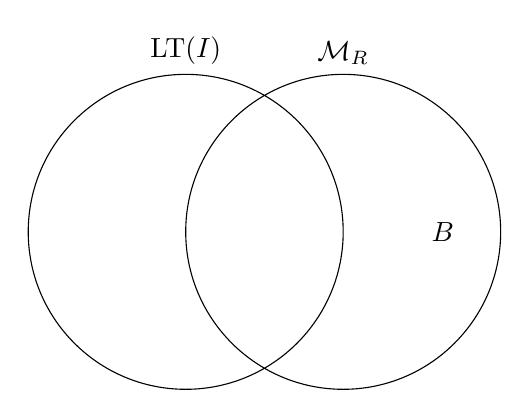
\begin{tikzpicture}
          \draw (-1, 0 ) circle (2)
                (-1, 2 ) node [above] {$\LT(I)$}
                ( 1, 0 ) circle (2)
                ( 1, 2 ) node [above] {$\cal M_R$}
                ( 2, 0 ) node [right] {$B$};
        \end{tikzpicture}
      \end{center}
      
      Either $\LT(f) \in B$ or $\LT(f) \in \LT(I)$.
      In the first case, suppose $\LT(f) = b \in B$.
      Then $f - b \in R - X$ has a smaller leading term than $f$,
      contradicting our choice of $f$.
      Otherwise, suppose $\LT(f) = m \in \LT(I)$.
      Then we can subtract from $f$ any monic polynomial in $I$ with the same leading term,
      again yielding a smaller polynomial in $R - X$.
  \end{description}
\end{proof}
\end{comment}

\begin{corollary}
  \label{cor_dim_R_mod_I}
  $$\dim_K R/I = \#\{ m \in \cal M_R ~|~ m \not\in \LT(I)\}.$$
\end{corollary}
\begin{theorem}
  Let $G = \{g_1, \ldots, g_m\}$ be a Gr\"obner basis and consider the system of polynomial equations
  \[g_1 = \ldots = g_m = 0.\]
  This system has finitely many solutions if and only if for every indeterminate $x_i \in K[x_1, \ldots, x_n]$,
  there is a power $x_i^k$ and element $g \in G$ such that $\LM(g) = x_i^k$.
\end{theorem}
\begin{proof}
  \S 3.6 of \cite{buchberger98}.
\end{proof}

\begin{theorem}
  Let $G = \{g_1, \ldots, g_m\}$ be a Gr\"obner basis and suppose the system of polynomial equations
  \[g_1 = \ldots = g_m = 0\]
  has finitely many solutions.
  Let $N$ be the number of solutions.
  \begin{enumerate}[label=(\roman*)]
    \item $N = \#\{ m \in \cal M_R ~|~ m \not\in \pid{\LT(g_1), \ldots, \LT(g_m)} \}$.
    \item If $I$ is the $R$-ideal generated by $G$, then $N = \dim_K R/I$.
  \end{enumerate}
\end{theorem}
\begin{proof}
  For part (i), see \S 3.6 of \cite{buchberger98}.
  Part (ii) follows from Corollary \ref{cor_dim_R_mod_I}.
\end{proof}
\begin{comment}
\begin{theorem}
  \label{thm_groebner_basis_product}
  Let $I$ and $J$ be ideals of $R = K[x_1, \ldots, x_n]$, generated by Gr\"obner bases, say
  \begin{align*}
    I &= \pid{f_1, \ldots, f_m} \\
    J &= \pid{g_1, \ldots, g_n}.
  \end{align*}
  Then
  \[ \{ f_ig_j ~|~ 1 \leq i \leq m, 1 \leq j \leq n \} \]
  is a Gr\"obner basis for the ideal product $IJ$.
\end{theorem}
\begin{proof}
  \begin{align*}
    \LT(IJ)
      &= \pid{ \LT(h) ~|~ h \in IJ } \\
      &= \pid{ \LT(fg) ~|~ f \in I, g \in J } \\
      &= \pid{ \LT(f)\LT(g) ~|~ f \in I, g \in J } \\
      &= \pid{ \LT(f) ~|~ f \in I } \pid{ \LT(g) ~|~ g \in J } \\
      &= \LT(I) \LT(J) \\
      &= \pid{ \LT(f_i) ~|~ 1 \leq i \leq m } \pid{ \LT(g_j) ~|~ 1 \leq j \leq n } \\
      &= \pid{ \LT(f_i) \LT(g_j) ~|~ 1 \leq i \leq m, 1 \leq j \leq n } \\
      &= \pid{ \LT(f_i g_j) ~|~ 1 \leq i \leq m, 1 \leq j \leq n }
  \end{align*}
\end{proof}
\end{comment}

\begin{theorem}
  \label{thm_groebner_basis_remainder}
  Let $I$ be an ideal of $R$, generated by the Gr\"obner basis $G = \{ g_1, \ldots, g_m \}$. Then,
  \begin{enumerate}[label=(\roman*)]
    \item
    Every polynomial $f \in R$ can be written uniquely in the form
    \begin{equation*}
      f = g + r
    \end{equation*}
    where $g \in I$, $r \in R$, and $r$ is reduced modulo $G$.

    \item
    For any polynomial $f \in R$, we have that $f \in I$ if and only if $r = 0$.
  \end{enumerate}
\end{theorem}
\begin{proof}
  Chapter 2, \S 6, Proposition 1 and Corollary 2 in \cite{cox07}.
\end{proof}

\begin{comment}
It is an obvious fact that, given any polynomial $f \in K[x_1, \ldots, x_n]$,
we can separate $f$ into its homogeneous components.
That is, we can write
\[ f = \sum_{i = 0}^n f_i^* \]
where $n$ is the total degree of $f$ and $f_i^*$ is homogeneous of degree $i$.

Given a point $P = (a_1, \ldots, a_n) \in \bb A_K^n$, we can even write $f$ in the same form,
but where $f_i^*$ is homogeneous in the variables $(x_1 - a_1), \ldots, (x_n - a_n)$.
E.g., in $\bb Q[x,y]$, given the point $P = (1,1)$, 
\[ x^2 + y^2 = [(x - 1)^2 + (y - 1)^2] + [2(x + 1) + 2(y + 1)] + [2]. \]
This is just the multivariate Taylor series expansion of the polynomial around the point $P$.
This generalizes to the following.

\begin{theorem}
  Let $R = K[x_1, \ldots, x_n]$ and let $I$ be an ideal of $R$ given by a Gr\"obner basis $I = \pid{g_1, \ldots, g_m}$.
  Then $f$ can be written uniquely in the form
  \[ f = \sum_{i=0}^t f_i^*, \]
  where $t = \max\{n \in \bb N ~|~ f \in I^n\}$, $f_i^* \in I^i - I^{i+1}$, and $f_i^* \not\in \LT(I^{i+1})$.
\end{theorem}
\begin{proof}
  By Theorem \ref{thm_groebner_basis_product}, our Gr\"obner basis for $I$ gives us a basis for $I^t$.
  Theorem \ref{thm_groebner_basis_remainder} then applies, allowing us to write
  \[ f = f^*_t + r_t \]
  with $f^*_t \in I^t - I^{t+1}$ and $r_t \in R$, $r_t \not\in \LT(I^t)$.
  Applying Theorems \ref{thm_groebner_basis_product} and \ref{thm_groebner_basis_remainder} $t-1$ more times gives the result.
\end{proof}

Essentially, given finitely polynomials $\{ g_i \}$ forming a Gr\"obner basis for an ideal,
we can uniquely perform a homogenous decomposition of any polynomial $f$ with respect to the $g_i$'s.

This also allows us to show that (over a field of sufficiently large characteristic)
$f \in I^2$ if and only if $f$ and its differential $df$ vanish modulo $I$.
\end{comment}



%%%%%%%%%%%%%%%%%%%%%%%%%%%%%%%%%%%%%%%%%%%%%%%%%%
%%%%%                                        %%%%%
%%%%%   Groebner Bases in Coordinate Rings   %%%%%
%%%%%                                        %%%%%
%%%%%%%%%%%%%%%%%%%%%%%%%%%%%%%%%%%%%%%%%%%%%%%%%%

\subsection{Gr\"obner Bases in Coordinate Rings}
\label{sec_groebner_bases_in_coordinate_rings}

While the theory of Gr\"obner bases always takes place in polynomial rings,
the theory may be extended to the coordinate ring of a $C_{3,4}$ curve,
though the equivalence relation leads to a complication.
Take, for example, the ring $K[x,y]$ for some field $K$ with the $C_{3,4}$ monomial order.
Then $x^4 < y^3$ in $K[x,y]$.
Now consider the coordinate ring $K[C] := K[x,y]/\pid{y^3 + x^4 + 1}$
(supposing this curve is non-singular).
This places a relation on $1$, $x^4$, and $y^3$.
How can we compare the monomials $y^3$ and $x^4$ in $K[C]$ if $y^3 \equiv -x^4 - 1$?
Given that $y$ divides $x^4 + 1$ in $K[C]$, is $\pid{y, x^4 + 1}$ a reduced Gr\"obner basis in $K[C]$ or not?
We must therefore make clear what we mean by a Gr\"obner basis in a coordinate ring.

Let $R = K[x,y]$ be a bivariate polynomial ring with some fixed monomial order $\leq$.
Let $f \in R$ be irreducible over $K$ and let $K[C] = R/\pid f$.
Then the ideals of $R$ containing $f$ are in bijection with the ideals of $K[C]$
(Theorem III.2.13 in \cite{hungerford}).
Let $G = \pid{g_1, \ldots, g_m}$ be a finite subset of $K[C]$
and let $I = \pid G$ be the $K[C]$-ideal generated by $G$.
Let $\bar f \in R$ be the reduction of $f \in R$ modulo $G$, in the sense of Definition \ref{def_reduced_polynomial},
and treating $G$ as a subset of $R$.
We will say that $G$ is a Gr\"obner basis for $I$ if the set $G \cup \{ \bar f \}$ is a Gr\"obner basis in $K[x,y]$.

In each of the examples below,
let $K = \bb F_{11}$,
let $R = K[x,y]$ with the $C_{3,4}$ order,
and let $f = y^3 + x^4 + 1$ and $K[C] = R/\pid f$.
\begin{example}
  Consider the ideal $I = \pid{x^2 + x, xy} \subset K[C]$.
  The set $G = \{ x^2 + x, xy \}$ is \emph{not} a Gr\"obner basis for $I$.
  
  The reduction of $f$ modulo its generators is
  \begin{align*}
    \bar f  &= y^3 + x^4 + 1 \\
            &\equiv y^3 - x^3 + 1 & \text{reduce modulo $x^2 + x$} \\
            &\equiv y^3 + x^2 + 1 & \text{reduce modulo $x^2 + x$} \\
            &\equiv y^3 - x + 1 & \text{reduce modulo $x^2 + x$}.
  \end{align*}
  Now we lift $I$ to $I^* = \pid{x^2 + x, xy, y^3 - x + 1} \subset R$.
  However, one of the $S$-polynomials of the generators of $I^*$ does not reduce to 0 modulo $G$.
  \begin{align*}
    S(x^2 + x, y^3 - x + 1)
      &= (x^2 + x)\frac{x^2y^3}{x^2} - (y^3 - x + 1)\frac{x^2y^3}{y^3} \\
      &= xy^3 + x^3 - x^2 \\
      &\equiv x^3 - x^2 & \text{reduce modulo $xy$} \\
      &\equiv -2x^2 & \text{reduce modulo $x^2 + x$} \\
      &\equiv 2x \pmod G & \text{reduce modulo $x^2 + x$}.
  \end{align*}
  In fact, $I = \pid{x}$ and $\{x\}$ is a Gr\"obner basis in $K[C]$.

  By contrast, $\{x^2 + x, xy\}$ \emph{is} a Gr\"obner basis of $K[x,y]$,
  as per Example \ref{ex_groebner_2}.
\end{example}
\begin{example}
  Consider instead $I = \pid{y^2} \subset K[C]$.
  The reduction of $f$ modulo $y^2$ is $\bar f = x^4 + 1$.
  Lift $I$ to $I^* = \pid{y^2, x^4 + 1} \subset R$.
  There is only one $S$-polynomial to consider on the generators of $I^*$,
  \[ S(y^2, x^4 + 1) = (y^2) \frac{x^4y^2}{y^2} - (x^4 + 1)\frac{x^4y^2}{x^4} = y^2. \]
  This $S$-polynomial reduces to 0 modulo $\{y^2, x^4 + 1\}$,
  hence $\{y^2, x^4 + 1\}$ is a Gr\"obner basis in $K[x,y]$ and $\{y^2\}$ is a Gr\"obner basis in $K[C]$.
  
  This example illustrates the need to compute the reduction $\bar f$ of $f$ modulo $G$,
  since $\{y^2, x^4 + 1\}$ is a Gr\"obner basis in $K[x,y]$, but $\{y^2, y^3 + x^4 + 1\}$ is not.
\end{example}
  
%%%%%%%%%%%%%%%%%%%%%%%%%%%
%%%%%                 %%%%%
%%%%%   Derivations   %%%%%
%%%%%                 %%%%%
%%%%%%%%%%%%%%%%%%%%%%%%%%%

\section{Differential Forms}
\label{chap_differentials}

In a typical undergraduate mathematics curriculum,
derivatives and differential forms appear in the study of real- or complex-valued functions.
In real and complex analysis courses,
it is seen that $\bb R$ and $\bb C$ are complete with respect to their standard metrics.
Concepts such as limits, convergence, and derivatives are defined with respect to these metrics.
In this thesis, we wish to speak of derivatives and differentials of functions that are not real-valued,
but rather members of a polynomial ring $K[x,y]$ over a finite field or a quotient of that polynomial ring.
It is not so clear anymore what is meant by the differential of a polynomial in these discrete spaces.

In this chapter, we define (K\"ahler) differentials of functions purely algebraically
in a sufficient generality as to cover differentials of polynomials in $A = R[x_1, \ldots, x_n]$,
multivariate polynomials with coefficients in a commutative ring with identity $R$.
We will see how to extend this definition to differentials on functions in other spaces constructed from $A$,
such that its field of fractions, quotients, and localizations.
Along the way, we give a natural definition of the formal derivative and formal partial derivative.

The contents of this chapter come mostly from a combination of the books
\cite{eisenbud95}, \cite{eisenbud00}, \cite{goldschmidt03}, and \cite{stichtenoth09}.



%%%%%%%%%%%%%%%%%%%%%%%%%%%
%%%%%                 %%%%%
%%%%%   Derivations   %%%%%
%%%%%                 %%%%%
%%%%%%%%%%%%%%%%%%%%%%%%%%%

\subsection{Derivations}
\begin{definition}
  Let $R$ be a \note{commutative?} ring, $A$ an $R$-algebra, and $M$ an $A$-module.
  A map $\delta : A \to M$ is called a \defn{derivation} (from $A$ to $M$)
  if it is $R$-linear and satisfies the product rule
  (also called the Leibniz rule):
    \[ \delta(ab) = \delta(a)b + a\delta(b). \]
\end{definition}

Some authors do not require a derivation to be $R$-linear,
and they distinguish between derivations and $R$-linear derivations.
We will assume all derivations are $R$-linear.

As the name suggests, many familiar properties of the derivative from calculus
are an immediate consequence of this definition.
The following are easily verified.
\begin{proposition}
  \label{prop_derivation}
  A derivation satisfies the following properties.
  \begin{enumerate}[label=(\roman*)]
    \item If $A$ is unital, then $\delta(1) = 0$.
    \item If $A$ is unital, then $\delta(r) = 0$ for all $r \in R$.
    \item If $A$ is commutative, then $\delta(x^2) = 2x\delta(x)$.
    \item If $A$ is commutative, then for all integers $n > 0$, $\delta(x^n) = nx^{n-1}\delta(x)$.
    \item If $x$ is a unit, then $\delta(x\inv) = -x^{-2}\delta(x)$.
    \item If $x$ is a unit, then for all $n \in \bb Z$, $\delta(x^n) = nx^{n-1}\delta(x)$.
    \item If $y$ is a unit, then $\delta(xy\inv) = (\delta(x)y - x\delta(y))y^{-2}$.
  \end{enumerate}
\end{proposition}
\begin{comment}
\begin{proof}
  \begin{enumerate}[label=(\roman*)]
    \item
      We have
        \[ D(1) = D(1 \cdot 1) = D(1) \cdot 1 + 1 \cdot D(1) = D(1) + D(1) \]
      which implies $D(1) = 0$.
    \item
      Follows from (i) by $R$-linearity.
    \item
        \[ D(x^2) = D(x)x + xD(x) = xD(x) + xD(x) = 2xD(x). \]
    \item
      Follows from (iii) by induction.
      Suppose $D(x^k) = kx^{k-1}D(x)$ for some $k > 0$. Then
      \begin{align*}
        D(x^{k+1})
          &= D(x^k \cdot x) \\
          &= D(x^k)x + x^kD(x) \\
          &= kx^{k-1}D(x)x + x^kD(x) \\
          &= kx^kD(x) + x^kD(x) \\
          &= (k + 1)x^kD(x).
      \end{align*}
    \item
      By part (i) and the product rule, we have
        \[ 0 = D(1) = D(xx\inv) = D(x)x\inv + xD(x\inv). \]
      This implies
        \[ xD(x\inv) = -D(x)x\inv, \]
      hence
        \[ D(x\inv) = -x^{-2}D(x). \]
    \item
      The case where $n \geq -1$ is handled by parts (i), (iv), and (v).
      The rest follows by induction.
      Suppose $D(x^k) = kx^{k-1}D(x)$ for some $k \leq -1$. Then
      \begin{align*}
        D(x^{k-1})
          &= D(x^kx\inv) \\
          &= D(x^k)x\inv + x^kD(x\inv) \\
          &= kx^{k-1}D(x)x\inv - x^kx^{-2}D(x) \\
          &= kx^{k-2}D(x) - x^{k-2}D(x) \\
          &= (k - 1)x^{k-2}D(x).
      \end{align*}
    \item
      Immediate from the product rule and part (v).
      \begin{align*}
        D(xy\inv)
          &= D(x)y\inv + xD(y\inv) \\
          &= D(x)y\inv - xy^{-2}D(y) \\
          &= (D(x)y - xD(y))y^{-2}.
      \end{align*}
  \end{enumerate}
\end{proof}
\end{comment}

We can define the sum of two derivations $\delta_1$ and $\delta_2$ by
  \[ (\delta_1 + \delta_2)(x) = \delta_1(x) + \delta_2(x) \]
and scalar multiplication of a derivation $\delta$ by a ring element $r$ by
  \[ (r\delta)(x) = r\delta(x). \]
Under these operations, the set of derivations from $A$ to $M$ becomes an $R$-module,
denoted by $\Der_R(A,M)$.
This is the \defn{module of derivations from $A$ to $M$}.
In the case where $M = A$, this may be denoted by $\Der_R(A)$.

Property (v) of Proposition \ref{prop_derivation} shows that if $x$ is a unit,
then $\delta(x\inv)$ is determined by $\delta(x)$.
This suggests that there is a relationship between derivations from an algebra $A$
and derivations from the field of fractions of $A$,
although note that $A$ must not have any zero divisors in order for its field of fractions to be constructed.

\begin{proposition}
  \label{prop_derivation_unique_extension}
  Let $A$ be an $R$-algebra with no zero divisors and let $\delta \in \Der_R(A,M)$.
  Let $B = \Frac A$, the field of fractions of $A$.
  There is a unique $\delta' \in \Der_R(B, M)$ whose restriction to $A$ is $\delta'|_A = \delta$.
\end{proposition}
That is to say that if $\delta$ is a derivation from $A$ to $M$,
it extends uniquely to a derivation from $\Frac A$.
\begin{proof}
  If $A = B$, we are done.
  So suppose instead there is a $b \in B$ such that $b\in A$ but $b\inv \not \in A$.
  Suppose $\delta_1, \delta_2 \in \Der_R(B, M)$ are such that $\delta_1|_{A} = \delta = \delta_2|_{A}$.
  Then $\delta_1(b) = \delta(b) = \delta_2(b)$ and
    \[ \delta_1(b\inv) = -b^{-2}\delta_1(b) = -b^{-2}\delta_2(b) = \delta_2(b\inv). \]
  It follows that $\delta_1(ab\inv) = \delta_2(ab\inv)$ for all $ab\inv \in B$.
\end{proof}

In order to understand how a derivation acts on $\Frac A$, it is enough to know how it acts on $A$.
In the case of a derivation over the field $R(x_1, \ldots, x_n)$,
it is enough to know how it acts on the polynomial ring $R[x_1, \ldots, x_n]$.
In the univariate case, we can say even more.
The behaviour of a derivation $\delta: R(x) \to M$ is entirely determined by the value of $\delta(x)$.

\begin{proposition}
  \label{prop_derivation_unique_x}
  Let $R(x)$ be the ring of rational functions over a ring $R$ in a single variable $x$.
  Let $\delta_1, \delta_2 \in \Der_R(R(x))$.
  If $\delta_1(x) = \delta_2(x)$, then $\delta_1 = \delta_2$.
\end{proposition}
\begin{proof}
  For all $r \in R$, we have $\delta_1(r) = \delta_2(r) = 0$.
  For all $f \in R[x]$, we have $\delta_1(f) = \delta_2(f)$ by $R$-linearity.
  Now $\delta_1$ and $\delta_2$ agree on all of $R[x]$.
  By Proposition \ref{prop_derivation_unique_extension}, they must agree on all of $R(x)$.
\end{proof}

For a (unital) ring $R$, the \defn{formal derivative} on $R(x)$
is the unique derivation $D_x \in \Der_R(R(x))$ satisfying $D_x(x) = 1$.
The formal derivative of a function $f$ is often denoted $f' := D_x(f)$,
although this convention will not be adopted here ---
beyond this paragraph, this thesis has no use for derivations on univariate polynomials.
The formal derivative behaves exactly as one might expect.
\begin{example}
  Let $f = 3x^3 + 6x^2 + 1 \in \bb Z[x]$. Then
  \begin{align*}
    D_x(f) 
      &= 3D_x(x^3) + 6D_x(x^2) + D_x(1) & R\text{-linearity} \\
      &= 3 \cdot 3 x^2 D_x(x) + 6 \cdot 2 x D_x(x) + 0 & \text{Proposition \ref{prop_derivation}}\\
      &= 9 x^2 + 12 x & D_x(x) = 1.
  \end{align*}
\end{example}

\begin{comment}
Up to this point, we have discussed derivations without showing that such a thing even exists.
The following proposition establishes the existence of derivations by exhibiting one that should be familiar.

\begin{proposition}
  \label{prop_derivation_formal_derivative}
  Let $R(x)$ be the ring of rational functions over a ring $R$ in a single variable $x$.
  There is a unique derivation $D_x : R(x) \to R(x)$ satisfying $D_x(x) = 1$.
\end{proposition}
Given a rational function $f(x)$, the function $D_x(f(x))$ is the \defn{formal derivative} of $f(x)$, often written $f'(x)$.
\begin{proof}
  We need only show existence of a derivation on $R[x]$ with the desired property.
  By propositions \ref{prop_derivation_unique_extension} and \ref{prop_derivation_unique_x},
  this derivation is unique and extends uniquely to a derivation on $R(x)$ with the desired property.
  
  We set $D_x(x) = 1$ and extend by linearity to get its action on all of $R[x]$.
  If $f(x) = \sum f_ix^i \in R[x]$, then
    \[ D(f(x)) = \sum if_ix^{i-1}D(x) = \sum if_ix^{i-1}. \]
  We must show that this satisfies the product rule.
  Let $g(x) = \sum g_jx^j$. Then for all $f(x), g(x) \in R[x]$,
  
  \begin{align*}
    D_x(f(x)g(x))
      &= D_x \left( \left( \sum_{i=0}^m f_ix^i \right) \left( \sum_{j=0}^n g_jx^j \right) \right) \\
      &= D_x \left( \sum_{i=0}^m \sum_{j=0}^n f_ix^i g_jx^j \right) \\
      &= D_x \left( \sum_{i=0}^m \sum_{j=0}^n f_ig_jx^{i+j} \right) \\
      &= \sum_{i=0}^m \sum_{j=0}^n f_ig_jD_x(x^{i+j}) \\
      &= \sum_{i=0}^m \sum_{j=0}^n (i+j)f_ig_jx^{i+j-1} \\
      &= \sum_{i=0}^m \sum_{j=0}^n (if_ig_jx^{i+j-1} + jf_ig_jx^{i+j-1}) \\
      &= \sum_{i=0}^m \sum_{j=0}^n if_ig_jx^{i+j-1} + \sum_{i=0}^m \sum_{j=0}^n jf_ig_jx^{i+j-1} \\
      &= \left( \sum_{i=0}^m if_ix^{i-1} \right) \left( \sum_{j=0}^n g_jx^j \right) + \left( \sum_{i=0}^m f_ix^i \right) \left( \sum_{j=0}^n jg_jx^{j-1} \right) \\
      &= D_x(f(x)) g(x) + f(x)D(g(x)).
  \end{align*}
\end{proof}
\end{comment}

Now consider the $R$-algebra $A = R(x_1, \ldots, x_n)$, rational functions in $n$ variables.
For each $1 \leq i \leq r$,
we can set $S_i = R(x_1, \ldots, x_{i-1}, x_{i+1}, \ldots, x_n)$, so that $A = S_i(x_i)$.
We have merely realized $A$ as the algebra of rational functions in one variable $x_i$ and coefficients in $S_i$,
which is the algebra of rational functions in the other $n - 1$ variables.
Then Proposition \ref{prop_derivation_unique_x} says that
there is a unique derivation $D_{x_i} \in \Der_{S_i}(A)$ satisfying $D_{x_i}(x_i) = 1$.
This derivation $D_{x_i}$ is also a member of $\Der_R(A)$ and its action on the other indeterminates of $A$ is
\begin{align*}
  D_{x_i}(x_j) &= \begin{cases} 1 & i = j \\ 0 & i \neq j \end{cases}.
\end{align*}
The requirement that $D_{x_i}(x_j) = 0$ when $i \neq j$ is a consequence of $S_i$-linearity
by $D_{x_i}$'s membership in $\Der_{S_i}(A)$.
If $f \in A$, then $f_{x_i} := D_{x_i}(f)$ is the \defn{formal partial derivative} with respect to $x_i$.

\begin{example}
  In the case of $A = \bb Z[x,y]$, we have derivations $D_x$ and $D_y$ with
  $D_x(x) = 1 = D_y(y)$ and $D_x(y) = 0 = D_y(x)$.
  Let $f = x^2 + xy + y^3 \in A$.
  Then $f_x = D_x(f) = 2x + y$ and $f_y = D_y(f) = x + 3y^2$.
\end{example}

\begin{comment}
\begin{proposition}
  Let $D \in \Der_K(A)$ be a derivation.
  Let $I$ be an ideal of $A$.
  Then $D$ induces a derivation $D^* \in \Der_K(A/I)$ defined by
    \[ D^*([a]) = [D(a)]. \]
\end{proposition}
\begin{proof}
  For each $a \in A$, denote the equivalence class containing $a$ in $A/I$ by $\bar a$.
  We show first that this map is well-defined.
  Suppose $\bar a = \bar b$.
  Then $\bar{a-b} = \bar 0$ and
    \[ D^*(\bar a) = D^*(\bar a - \bar{a-b}) = D^*(\bar{a-a+b}) = D^*(\bar b). \]
  We must also show that $D^*(\bar k \cdot \bar a) = \bar k \cdot D^*(\bar a)$
  and $D^*(\bar a \cdot \bar b) = D^*(\bar a) \cdot \bar b + \bar a \cdot D^*(\bar b)$.
    \[ D^*(\bar k \cdot \bar a) = D^*(\bar{ka}) = \bar{D(ka)} = \bar{kD(a)} = \bar k \cdot \bar{D(a)} = \bar k \cdot D^*(\bar a) \]
  \begin{align*}
    D^*(\bar a \cdot \bar b)
      &= D^*(\bar{ab})
       = \bar{D(ab)}
       = \bar{D(a)b + aD(b)} \\
       &= \bar{D(a)} \cdot \bar b + \bar a \cdot \bar{D(b)}
       = D^*(\bar a) \cdot \bar b + \bar a \cdot D^*(\bar b)
  \end{align*}
\end{proof}
With this we can extend formal derivatives of functions in $K[x,y]$ and $K(x,y)$ to formal derivatives of functions in $K[C]$ and $K(C)$.
\end{comment}

We may compose derivations with a morphisms of algebras to obtain new derivations.

\begin{proposition}
  \label{prop_precompose_derivation}
  Let $f \in \Hom_R(A,B)$ be a morphism of $R$-algebras and let $\delta \in \Der_R(B,M)$ be an $R$-linear derivation.
  \[ \begin{tikzcd} A \arrow{r}{f} & B \arrow{r}{\delta} & M \end{tikzcd} \]
  Then $\delta \circ f \in \Der_R(A,M)$.
\end{proposition}
\begin{proof}
  While $M$ is a $B$-module, it becomes an $A$-module under the $A$-action
    \[ A \times M \to M : (a, m) \mapsto f(a)m. \]
  Both $f$ and $\delta$ are $R$-linear, so $\delta \circ f$ is also $R$-linear.
  As for the product rule, let $a, b \in A$. Then
  \begin{align*}
    (\delta \circ f)(ab)
      &= \delta(f(ab)) \\
      &= \delta(f(a)f(b)) \\
      &= \delta(f(a))f(b) + f(a)\delta(f(b)) \\
      &= (\delta \circ f(a))f(b) + f(a)(\delta \circ f(b)) \\
      &= (b, \delta \circ f(a)) + (a, \delta \circ f(b)). \qedhere
  \end{align*}
\end{proof}



%%%%%%%%%%%%%%%%%%%%%%%%%%%%%%%%%%%%
%%%%%                          %%%%%
%%%%%   Universal Derivation   %%%%%
%%%%%                          %%%%%
%%%%%%%%%%%%%%%%%%%%%%%%%%%%%%%%%%%%

\subsection{K\"ahler Differentials}
\label{sec_kahler_differentials}

In this section, we briefly present a construction of K\"ahler differentials and some important properties.
For more detail, as well as alternative constructions,
see \cite{eisenbud95}, \cite{eisenbud00}, \cite{goldschmidt03}, or \cite{stichtenoth09}.

Let $A$ be an $R$-algebra.
The \defn{module of K\"ahler differentials} of $A$ over $R$,
denoted by $\Omega_{A/R}$,
is the $A$-module generated by the set $\{ d(a) ~|~ a \in A \}$,
where $d(a)$ is merely a symbol,
modulo the relations
\begin{align*}
  d(ab) &= d(a)b + ad(b) \\
  d(ra + sb) &= rd(a) + sd(b)
\end{align*}
for all $r, s \in R$ and $a, b \in A$.
The elements of $\Omega_{A/R}$ are called \defn{differential forms} or \defn{K\"ahler differentials}.
We will write $d(a)$ as simply $da$, though we will not write $d(ab)$ as $dab$, as this may be confused with $d(a)b$.
The map
  \[ d_A : A \to \Omega_{A/R} : a \mapsto d(a) \]
is an $R$-linear derivation, called the \defn{universal derivation}.
It is universal in the following sense.
If $\delta : A \to M$ is another $R$-linear derivation from $A$,
then there is a unique morphism of $R$-modules $\phi : \Omega_{A/R} \to M$ such that
\[ \begin{tikzcd}
  A \arrow{r}{d_A} \arrow[swap]{dr}{\delta} & \Omega_{A/R} \arrow[dashed]{d}{!\exists \phi} \\ & M
\end{tikzcd} \]
commutes.
This map is defined by $\phi : da \mapsto \delta(a)$.
We will omit the subscript and write $d$ in place of $d_A$,
except in contexts where there are multiple $d$'s and we need to distinguish them by their domains.

\begin{comment}
\begin{proposition}
  A morphism $\phi : A \to B$ of $R$-algebras induces
  a morphism $\psi : \Omega_{A/R} \to \Omega_{B/R}$ of $A$-modules.
\end{proposition}
\begin{proof}
  Let $\phi : A \to B$ be a morphism of $R$-algebras.
  We have the following maps,
  \[ \begin{tikzcd}
      A \arrow{r}{d_A} \arrow[swap]{d}{\phi} & \Omega_{A/R} \\ B \arrow[swap]{r}{d_B} & \Omega_{B/R}.
    \end{tikzcd} \]
  By Proposition \ref{prop_precompose_derivation},
  the composition $d_B \circ \phi : A \to \Omega_{B/R}$ is an $R$-linear derivation.
  By the universal property of the universal derivation,
  there is a unique map $\psi : \Omega_{A/R} \to \Omega_{B/R}$ such that
  \[ \begin{tikzcd}
      A \arrow{r}{d_A} \arrow[swap]{dr}{d_B \circ \phi} & \Omega_{A/R} \arrow[dashed]{d}{\psi} \\ & \Omega_{B/R}
    \end{tikzcd} \]
  commutes.
\end{proof}
The induced map sends $d_Aa \mapsto d_B(\phi(a))$.
\end{comment}

Of particular interest to us in this thesis is the case where $A = R[x_1, \ldots, x_n]$ is a polynomial ring.
In this case, $\Omega_{A/R}$ is the free $A$-module generated by the symbols $dx_1, \ldots, dx_n$.
\begin{proposition}
  \label{prop_differential_module_of_polynomial_ring}
  Let $A = R[x_1, \ldots, x_n]$. Then
  \[ \Omega_{A/R} \cong \bigoplus_{i=1}^n Adx_i. \]
\end{proposition}
\begin{comment}
\begin{corollary}
  Let $A = R[x_1, \ldots, x_n]$, let $I$ be an ideal of $A$, and let $B = A/I$.
  Then $B$ is an $R$-algebra and
  \[ B \otimes_{R} \Omega_{A/R} \cong \bigoplus_{i=1}^n Bdx_i. \]
\end{corollary}
\begin{proof}
  \note{Extension of scalars.}
\end{proof}
Here $\otimes_R$ denotes the tensor product of algebra.
We will use this corollary in Chapter \ref{chap_curves}, after defining the coordinate ring of a curve,
when relating differentials forms of a polynomial ring to those of a coordinate ring.
Since $\Omega_{A/R}$ is a direct sum of $R$-algebras $Adx_i$,
there is a family of natural projection maps 
  \[ \pi_i : \Omega_{A/R} \to Adx_i : \sum f_jdx_j \mapsto f_idx_i. \]
We can compose the maps
  \[ \begin{tikzcd}
    A \arrow{r}{d} & \Omega_{A/R} \arrow{r}{\pi_i} & Adx_i \arrow{r}{} & A
  \end{tikzcd} \]
where the right-most map sends $dx_i \mapsto 1$.
The composition of the three maps is the formal partial derivative with respect to $x_i$.
\end{comment}



%%%%%%%%%%%%%%%%%%%%%%%%%%%%%%%%%%%%%%%%%%
%%%%%                                %%%%%
%%%%%   Differential Forms in K[C]   %%%%%
%%%%%                                %%%%%
%%%%%%%%%%%%%%%%%%%%%%%%%%%%%%%%%%%%%%%%%%

\subsection{Differential Forms in $K[C]$}
\label{sec_differentials_in_coordinate_ring}

In Section \ref{sec_kahler_differentials}, we defined $\Omega_{A/R}$,
the module of K\"ahler differentials on an $R$-algebra $A$.
The coordinate ring is a $K$-algebra, so let us describe the structure of $\Omega_{K[C]/K}$.
To do so, we will make use of the following proposition.

\begin{proposition}
  \label{prop_conormal_sequence}
  Let $\pi : A \to B$ be an epimorphism of $R$-algebras.
  Let $I = \ker \pi$.
  There is an exact sequence of $B$-modules
    \[ I/I^2 \xrightarrow{d} B \tensor A \Omega_{A/R} \xrightarrow{D\pi} \Omega_{B/R} \to 0 \]
  where $d : [f] \mapsto 1 \otimes df$ and $D\pi : b \otimes da \mapsto b(da)$.
\end{proposition}
\begin{proof}
  Proposition 16.3 in \cite{eisenbud95}.
\end{proof}

This proposition makes use of the tensor product of modules.
The tensor product will not be defined or discussed in this thesis;
one may consult \cite{dummit04}, \cite{eisenbud95}, or \cite{hungerford} for more on that topic.
We will take advantage of other results to turn the tensor product into a direct sum of modules.

To understand the structure of $\Omega_{K[C]/K}$,
we begin by noting that the canonical quotient map $q : K[x,y] \to K[C]$ is an epimorphism of $K$-algebras
whose kernel is $\ker q = \pid F$, the ideal of $K[x,y]$ generated by the defining polynomial of the curve.
Proposition \ref{prop_conormal_sequence} therefore applies, telling us that there is an exact sequence
\begin{center}
\begin{tikzcd}
  \frac{\pid{F}}{\pid{F^2}} \arrow{r}{d} &
  K[C] \tensor {K[x,y]} \Omega_{K[x,y]/K} \arrow{r}{Dq} &
  \Omega_{K[C]/K} \arrow{r}{} &
  0.
\end{tikzcd}
\end{center}
Using a property of exact sequences (see remarks on page 176 of \cite{hungerford}), 
\[ \Omega_{K[C]/K} \cong \frac {K[C] \tensor {K[x,y]} \Omega_{K[x,y]/K}} {\im d}. \]
Next applying Proposition \ref{prop_differential_module_of_polynomial_ring},
\[ \Omega_{K[C]/K} \cong \frac {K[C] \tensor {K[x,y]} \Omega_{K[x,y]/K}} {\im d}
                   \cong \frac {K[C] \tensor {K[x,y]} (K[x,y]dx \oplus K[x,y]dy)} {\im d}. \]
The tensor product distributes over addition (Theorem IV.5.9 \cite{hungerford}), giving
\[ \Omega_{K[C]/K} \cong \frac {\left(K[C] \tensor {K[x,y]} K[x,y]dx\right) \oplus
                                \left(K[C] \tensor {K[x,y]} K[x,y]dy\right)} {\im d}. \]
A basic property of the tensor product is that a $R$-module $A$ tensored with its ring $R$ is isomorphic to itself,
i.e. $A \tensor R R \cong A$ (Theorem IV.5.7 \cite{hungerford}), hence
\[ \Omega_{K[C]/K} \cong \frac {K[C]dx \oplus K[C]dy} {\im d}. \]

To determine the image of $d$, it is enough to know the image of the element $F \in \pid F / \pid{F^2}$.
The element $F \in F \in \pid F / \pid{F^2}$ maps to $1 \otimes dF \in K[C] \otimes \Omega_{K[x,y]/K}$.
Following the chain of isomorphisms we just produced, this then maps to $F_xdx + F_ydy \in K[C]dx \oplus K[C]dy$.
Thus,
\[ \Omega_{K[C]/K} \cong \frac {K[C]dx \oplus K[C]dy} {\pid{F_xdx + F_ydy}}. \]
The module $\Omega_{K[C]/K}$ of differentials on $K[C]$ is generated by $dx$ and $dy$,
modulo the equivalence relation $F_xdx \equiv -Fydy$.
This relation between $dx$ and $dy$ means that it is therefore a rank 1 $K[C]$-module, generated by a single element.
\begin{proposition}
  \label{prop_differential_generator}
  There is a generator $dz$ for $\Omega_{K[C]/K}$ with the properties
  \begin{align*}
    dx &\equiv C_ydz \\
    dy &\equiv -C_xdz.
  \end{align*}
\end{proposition}
\begin{proof}
  See Lemma 5.1 in \cite{salem07}.
\end{proof}
In fact, there are many possible generators for $\Omega_{K[C]/K}$.
Another choice of generator allowing for more efficient doubling of typical divisors
will be presented in Chapter \ref{chap_doubling}.
The generator in Proposition \ref{prop_differential_generator} is a natural choice
that is useful for some proofs, and will be used in some atypical cases of divisor doubling.

The differential of a function $f \in K[C]$ with respect to this generator $dz$ is
\[ df = (f_xC_y - f_yC_x)dz. \]
If $I$ is an ideal of $K[C]$,
we will say by abuse of notation that $df \in I$ if $f_xC_y - f_yC_x \in I$.
Equivalently, we will say that $df \in I$ if $df$ vanishes modulo $I$.

Now let $\cal O_{\frak p}$ be the local ring at a prime ideal $\frak p$ of $K[C]$.
Then there is a map $d_{\cal O_{\frak p}} : \cal O_{\frak p} \to \Omega_{\cal O_{\frak p}/K}$.
The action of this map is inherited from the map $d_{K[C]} : K[C] \to \Omega_{K[C]/K}$.
That is, the differential of a function $f/g \in \cal O_{\frak p}$ is
\[ d_{\cal O_{\frak p}} \left( \frac f g \right) = \frac{d_{K[C]}(f)g - fd_{K[C]}(g)}{g^2}
 = \frac{(f_xC_y - f_yC_x)g - f(g_xC_y - g_yC_x)}{g^2} dz . \]
As noted earlier in this chapter, for readability, we will omit the subscripts on $d$
when it is clear in context which differential map is meant.

\begin{lemma}
  \label{lem_differential_of_uniformizer}
  Let $\frak p$ be a non-zero prime ideal of $\bar K[C]$.
  Let $u$ be a uniformizer for $\frak m_{\frak p}$, the maximal ideal of $\cal O_{\frak p}$.
  Then $du \not \in \frak m_{\frak p}$.
\end{lemma}
\begin{proof}
  Let $\frak p = \pid{x - x_0, y - y_0}$.
  Since $C$ is non-singular, the partial derivatives of $C$ are not simultaneously zero at $P = (x_0, y_0)$,
  so suppose without loss of generality that $C_y(x_0, y_0) \neq 0$.
  Then the tangent line to $C$ at $P$ is non-vertical and $u = x - x_0$ is a uniformizer for $\frak m_{\frak p}$.
  Then $du = dx = C_y \not\in \frak m_{\frak p}$.
\end{proof}
\begin{theorem}
  \label{thm_differential_increases_order}
  Let $\frak p$ be a non-zero prime ideal of $K[C]$ and $f$ a polynomial in $K[C]$.
  Suppose $\nu_{\frak p}(f) \geq n$ for some non-negative integer $n$. Then
  \[ \nu_{\frak p}(f) \geq n + 1 \iff \nu_{\frak p}(df) \geq n. \]
\end{theorem}
\begin{proof}
%\frak m_{\frak p}
  Let $u$ be a uniformizer for $\frak m_{\frak p}$.
  Then $f = au^n$ for some $a \in K(C)^*$, and
  \[ df = d(au^n) = u^nda + nau^{n-1}du. \]
  Now $u^nda \in \frak m_{\frak p}^n$,
  so $df \in \frak m_{\frak p}^n$ if and only if $nau^{n-1}du \in \frak m_{\frak p}^n$.
  But $n, du \not\in \frak m_{\frak p}$,
  so this is true if and only if $au^{n-1} \in \frak m_{\frak p}^n$. Hence
  \[ df \in \frak m_{\frak p}^n
    \iff au^{n-1} \in \frak m_{\frak p}^n
    \iff au^n \in \frak m_{\frak p}^{n+1}
    \iff f \in \frak m_{\frak p}^{n+1}. \qedhere \]
\end{proof}
\begin{comment}
\begin{theorem}
  Let $A = K[x_1, \ldots, x_n]$ and let $I$ be an ideal of $A$.
  If $f \in I^2$, then $f \equiv 0$ and $df \equiv 0$ modulo $I$.
\end{theorem}
\begin{proof}
  Let $f \in I^2$.
  Then $f \in I$, so $f \equiv 0 \pmod I$.
  As for its differential, we have that $f$ is generated by a Gr\"obner basis {$g_i$}
  \[ f = \sum a_{i,j}g_ig_j, \]
  so
  \begin{align*}
    df &= d \left( \sum_{\substack{1 \leq i \leq j \leq m}} a_{i,j}g_ig_j \right) \\
       &= \sum_{\substack{1 \leq i \leq j \leq m}} d \left( a_{i,j}g_ig_j \right) \\
       &= \sum_{\substack{1 \leq i \leq j \leq m}} \left( d(a_{i,j})g_ig_j + a_{i,j}d(g_i)g_j + a_{i,j}g_id(g_j) \right) \\
       &\equiv 0 \pmod I
  \end{align*}
\end{proof}

The converse is not true in general.
A simple counterexample is to let $A = \bb F_2[x]$, let $f = x^2$, and let $I = \pid f$.
Then $f \equiv 0 \pmod I$ and $df = 2xdx \equiv 0 \pmod I$.
However, $f \not\in I^2 = \pid{x^4}$.

It is true under additional assumptions.

\begin{theorem}
  Let $A = K[x_1, \ldots, x_n]$ and let $I$ be an ideal of $A$.
  Let $f \in A$ be a polynomial whose formal partial derivatives do not all vanish.
  If $f, df \equiv 0 \pmod I$, then $f \in I^2$.
\end{theorem}
\begin{proof}
  We prove the contrapositive.
  Suppose $f \not\in I^2$.
  If $f \not\equiv 0 \pmod I$, we are done, so suppose $f \equiv 0 \pmod I$ (i.e. $f \in I$).
  We wish to show that $df \not\equiv 0 \pmod I$.

  By Theorem \ref{thm_groebner_basis_remainder}, we can write $f$ as
  \[ f = g + r \]
  where $g \in I^2$ and $r \not\in \LT(I^2)$. Furthermore, $0 \neq r \in I$.
  Since $r \not\in \LT(I^2)$, $D_{x_k}(r) \not\in \LT(I^2)$ for any $1 \leq k \leq n$.
  \begin{align*}
    df &= dg + dr \\
       &\equiv dr \pmod I \\
       &= \sum D_{x_i}(r)dx_i
  \end{align*}
  We must argue now that for each summand $D_{x_i}(r)dx_i$ is non-zero modulo $I$.
  
  Suppose that $D_{x_k}(r) \equiv 0$ for some $1 \leq k \leq n$.
  \begin{align*}
    & D_{x_k}(r) \equiv 0 \pmod I \\
    \implies & D_{x_k}(r) \in I \\
    \implies & \LT(D_{x_k}(r)) \in \LT(I) \\
    \implies & \LT(D_{x_k}(r)) \in \LT(I)\LT(I) \\
    \implies & \LT(D_{x_k}(r)) \in \LT(I^2).
  \end{align*}
  However, as noted earlier, no term in $D_{x_k}(r)$ is in $\LT(I^2)$.
  \note{(Wording.)}
\end{proof}

\begin{proof}
  We prove the contrapositive.
  Suppose $f \not\in I^2$.
  If $f \not\equiv 0 \pmod I$, we are done, so suppose $f \equiv 0 \pmod I$ (i.e. $f \in I$).
  We wish to show that $df \not\equiv 0 \pmod I$.

  By Theorem \ref{thm_groebner_basis_remainder}, we can write $f$ as
  \[ f = g + r \]
  where $g \in I^2$ and $r \not\in \LT(I^2)$.
  Taking the differential of $f$,
  \begin{align*}
    df &= \sum_{i=1}^n D_{x_i}(f)dx_i.% \\
%       &= \sum_{i=1}^n D_{x_i}(g + r)dx_i \\
  \end{align*}
  We must show that one of $df$'s summands is non-zero modulo $I$.
  Since $f$ has a non-zero formal partial derivative, let $k$ be such that $D_{x_k}(f) \neq 0$.
  Then
  \begin{align*}
    D_{x_k}(f)
      &= D_{x_k}(g + r) \\
      &= D_{x_k}(g) + D_{x_k}(r) \\
      &\equiv D_{x_k}(r) \pmod I.
  \end{align*}
  Now suppose $D_{x_k}(r) \equiv 0 \pmod I$. Then
  \begin{align*}
    & D_{x_k}(r) \equiv 0 \pmod I \\
    \implies & D_{x_k}(r) \in I \\
    \implies & \LT(D_{x_k}(r)) \in \LT(I) \\
    \implies & \LT(D_{x_k}(r)) \in \LT(I)\LT(I) \\
    \implies & \LT(D_{x_k}(r)) \in \LT(I^2).
  \end{align*}
  %However, as noted earlier, no term in $D_{x_k}(r)$ is in $\LT(I^2)$.
  %\note{(Wording.)}
\end{proof}

\begin{proof}
  \note{(Supposing $I = \sqrt I$.)}
  We prove the contrapositive.
  Suppose $f \not\in I^2$.
  If $f \not\equiv 0 \pmod I$, we are done, so suppose $f \equiv 0 \pmod I$ (i.e. $f \in I$).
  We wish to show that $df \not\equiv 0 \pmod I$.

  By Theorem \ref{thm_groebner_basis_remainder}, we can write $f$ as
  \[ f = g + r \]
  where $g \in I^2$ and $r \not\in \LT(I^2)$.
  Taking the differential of $f$,
  \begin{align*}
    df &= dg + dr \\
       &\equiv dr \pmod I \\
       &= d\left(\sum_{i=1}^m a_ig_i \right) \\
       &\equiv \sum_{i=1}^m a_id(g_i) \pmod I.
  \end{align*}
\end{proof}



\begin{theorem}
  Let $\frak p$ be a prime ideal of $K[C]$.
  Let $f \in \frak p$.
  Then $f \in \frak p^2$ if and only if $df \in \frak p$.
\end{theorem}
\begin{proof}
  Let $r = \ord_{\frak p}f$. 
  Then $f$ may be written
  \[ f = \sum_{i=1}^r a_iu^i,\]
  where $u$ is a uniformizer of $\frak m_{\frak p}$ and $a_i \not\in \frak m_{\frak p}$. Then
  \begin{align*}
    df &= \sum_{i=1}^r d(a_iu^i) \\
       &= \sum_{i=1}^r (u^ida_i + a_id(u^i)) \\
       &= \sum_{i=1}^r (u^ida_i + ia_iu^{i-1}du) \\
       &= \sum_{i=1}^r u^ida_i + \sum_{i=0}^{r-1} (i+1)a_{i+1}u^idu.
  \end{align*}
  Now $df \in \frak p$ if and only if the $i=0$ term in the second sum is zero,
  i.e. if and only $a_1du = 0$.
  However, since $du \neq 0$, we have
  \[ df \in \frak p \iff a_1 = 0 \iff f \in \frak p^2. \]
\end{proof}
\end{comment}

%%%%%%%%%%%%%%%%%%%%%%%%
%%%%%              %%%%%
%%%%%   Divisors   %%%%%
%%%%%              %%%%%
%%%%%%%%%%%%%%%%%%%%%%%%

\section{The Divisor Class Group}
\label{chap_divisors}



\subsection{Divisors}

Let $C$ be a $C_{3,4}$ curve.
A \defn{divisor} $D$ of $C$ is a formal sum of points in $C(\bar K)$, including possibly the point at infinity, $P_\infty$.
If $P$, $Q$, and $R$ are points on the curve $C$, then examples of divisors include
  \[ \begin{array}{c} P + Q + R - 3P_\infty \\ P + 3Q - 2R \\ Q \\ 0 \end{array}. \]
More generally, a divisor has the form
  \[ D = \sum_{P \in C(\bar K)} n_P P,\]
where only finitely many $n_P$'s are non-zero.

A divisor is an element free Abelian group generated by the set of points $C(\bar K)$.
This Abelian group is denoted by $\Div(C)$.
Addition and negation are defined in the obvious way:
\[ \left( \sum_{P \in C(\bar K)} n_P P \right) + \left( \sum_{P \in C(\bar K)} m_P P \right) = \sum_{P \in C(\bar K)} (n_P + m_P) P \]
\[ -\left( \sum_{P \in C(\bar K)} n_P P \right) = \sum_{P \in C(\bar K)} (-n_P) P. \]

The coefficient $n_P$ of $P$ is the \defn{order} of the divisor $D$ at $P$, denoted by $\ord_P(D)$.
For example, if $D = P + 3Q - 2R$, then $\ord_Q(D) = 3$ and $\ord_R(D) = -2$.
The \defn{degree} of a divisor $D$, denoted by $\deg(D)$, is the sum of its orders at each point on the curve:
  \[ \deg(D) = \sum_{P \in C(\bar K)} \ord_P(D). \]
For example, $\deg(P + 3Q - 2R) = 1 + 3 - 2 = 2$.

It is easily verified that the map $\deg$ and the family of maps $\ord_P$ have the additive properties
  \[ \ord_P(A + B) = \ord_P(A) + \ord_P(B) \]
  \[ \deg(A + B) = \deg(A) + \deg(B). \]
In particular, $\ord_P$ and $\deg$ are group homomorphisms $\Div(C) \to \bb Z$.

We are able to put a partial order on divisors.
For two divisors $D = \sum n_P P$ and $D' = \sum m_P P$,
we order them
  \[ D \leq D' \iff \forall P \in C(\bar K) : n_P \leq m_P. \]
The divisor $D$ precedes $D'$ if it has lesser order than $D'$ at every point.
This partial order is compatible with addition, in the sense that for any divisors $A, B, D$,
  \[ A \leq B \implies A + D \leq B + D \]
  \[ A \leq B \implies -B \leq -A. \]
If $D \geq 0$, then $D$ is called an \defn{effective} divisor.

Divisors of a curve, together with this partial order, form a lattice --
every pair of divisors have a unique join and meet,
which we call their \defn{least common multiple} and \defn{greatest common divisor}.
Given two divisors $D$ and $D'$, their least common multiple is the unique, smallest divisor $L$ such that $D \leq L$ and $D' \leq L$.
Their greatest common divisor is the unique, largest divisors $G$ such that $G \leq D$ and $G \leq D'$.
Explicitly,
\begin{align*}
  \lcm(D, D') &= \sum_{P \in C(\bar K)}\max\{\ord_P(D), \ord_P(D')\}P \\
  \gcd(D, D') &= \sum_{P \in C(\bar K)}\min\{\ord_P(D), \ord_P(D')\}P.
\end{align*}
Just as integers $a$ and $b$ satisfy the law
  \[ \left| ab \right| = \lcm(a,b)\gcd(a,b), \]
divisors satisfy the law
  \[ D + D' = \lcm(D, D') + \gcd(D, D'). \]
This property will play a prominent role in adding divisors \note{in chapter ???}.

There is a short chain of subgroups of $\Div(C)$,
\[ \Princ(D) \subset \Div_K^0(C) \subset \Div^0(C) \subset \Div(C), \]
which we will now describe.

Since $\deg : \Div(C) \to \bb Z$ is a group homomorphism, its kernel is a subgroup of $\Div(C)$.
The kernel, of course, is the subgroup of divisors of degree zero, which we denote by $\Div^0(C) := \ker \deg$.

Let $\sigma \in \Gal(\bar K / K)$.
In \note{an earlier chapter}, we define the action of $\sigma$ of $C(\bar K)$.
This may be extended to an action on $\Div(C)$ in a natural way.
If $D = \sum n_P P$, then define
\[ \sigma(D) = \sum_{P \in C(\bar K)} n_P \sigma(P). \]
Just as $\sigma$ permutes points in $C(\bar K)$, so too does it permute divisors in $\Div(C)$.
In this way, an automorphism in $\Gal(\bar K/K)$ is also an automorphism of $\Div(C)$.

Given an automorphism $f$ on a group $G$, the \defn{fixed-point subgroup} of $f$ is
  \[ G^f := \{ g \in G ~|~ f(g) = g \}. \]
Given a set $S$ of automorphisms on $G$, this may be generalized even further:
  \[ G^S := \{ g \in G ~|~ \forall f \in S : f(g) = g \}. \]
So $G^S$ is the set of group elements in $G$ fixed by every automorphism in $S$.

We say that a divisor $D$ is \defn{defined over $K$} if $D$ is fixed by every automorphism in $\Gal(\bar K/K)$.
Divisors defined over $K$ therefore form a subgroup $\Div_K(C) \subset \Div(C)$.
  \[ \Div_K(C) := \Div(C)^{\Gal(\bar K/K)} \]

\begin{example}
  Let $K$ be any field, $L$ any algebraic extension and $\sigma \in \Gal(\bar K/L)$.
  By definition, $\sigma$ fixes $L$.
  If $P$ is any point with coordinates in $L$, then $\sigma(P) = P$.
  If $D$ is any divisor consisting only of points with coordinates in $L$, then $\sigma(D) = D$ and $D$ is defined over $L$.
\end{example}
\begin{example}
  Let $K = \bb F_2$ and let $L = K(\alpha)$ be an algebraic extension with $\alpha^2 + \alpha = 1$.
  Let $C$ be the curve $x^4 + y^3 + x + 1$ over $K$.
  Let $P$ be the point $(\alpha : 1 : 1)$ on $C$ and let $D$ be the divisor $D = P$.
  There is an automorphism $\sigma \in \Gal(\bar K/K)$ that maps $\alpha \mapsto \alpha + 1$, so 
    \[ \sigma(D) = \sigma(P) = (\sigma(\alpha) : \sigma(1) : \sigma(1)) = (\alpha + 1 : 1 : 1) \neq D. \]
  Hence $D$ is not defined over $K$.
\end{example}
\begin{example}
  Let $K$, $L$, $C$, and $P$ be as in the previous example.
  Let $Q = (\alpha + 1 : 1 : 1)$, which is also a point on $C$.
  Let $D$ be the divisor $D = P + Q$.
  Every automorphism $\sigma$ in $\Gal(\bar K/K)$ maps either $\alpha$ to itself or to $\alpha + 1$.
  In the former case,
  \begin{align*}
    \sigma(D) &= \sigma(P) + \sigma(Q) \\
              &= (\sigma(\alpha) : \sigma(1) : \sigma(1)) + (\sigma(\alpha + 1) : \sigma(1) : \sigma(1)) \\
              &= (\alpha : 1 : 1) + (\alpha + 1 : 1 : 1) \\
              &= P + Q = D.
  \end{align*}
  In the latter case,
  \begin{align*}
    \sigma(D) &= \sigma(P) + \sigma(Q) \\
              &= (\sigma(\alpha) : \sigma(1) : \sigma(1)) + (\sigma(\alpha + 1) : \sigma(1) : \sigma(1)) \\
              &= (\alpha + 1 : 1 : 1) + (\alpha : 1 : 1) \\
              &= Q + P = D.
  \end{align*}
  So $D$ is defined over $K$.
\end{example}

The intersection of subgroups is again a subgroup, so define
  \[ \Div_K^0(C) := \Div_K(C) \cap \Div^0(C). \]
These are the divisors defined over $K$ of degree zero.

If $f \in K(C)$ is a rational function on $C$,
then $f$ has finitely may zeros and poles along $C$, and,
counting multiplicities, there are as many zeros as there are poles.
\note{What theorem is this?}
Define the \defn{order} of $f$ at $P$ by
\[ \ord_P(f) = \begin{cases}
  n & \text{$f$ has a zero of order $n$ at $P$} \\
  -n & \text{$f$ has a pole of order $n$ at $P$}
\end{cases}. \]
Define the \defn{divisor of $f$} as
\[ \div(f) = \sum_{P \in C(\bar K)} \ord_P(f) P. \]
Since $f$ has finitely many zeros and poles, this formal sum belongs properly to $\Div(C)$,
thus it is correctly called a divisor.
Since these poles and zeros add to zero, this is a degree zero divisor.
\note{Need a proof that this is defined over $K$.}
Therefore $\div (f)$ is an element of $\Div_K^0(C)$.

If $D$ is a divisor and there is an $f$ such that $D = \div(f)$,
then $D$ is called a \defn{principal divisor}.
Principal divisors form a subgroup \note{(prove it is closed under addition)} $\Princ(C) \subset \Div_K^0(C)$.

Finally, we have describe the subsets
\[ \Princ(D) \subset \Div_K^0(C) \subset \Div^0(C) \subset \Div(C). \]
The \defn{divisor class group} of $C$ is the quotient group
\[ \Cl(C) = \frac {\Div_K^0(C)} {\Princ(C)}. \]
In the literature, the divisor class group is often called the \defn{Jacobian} $\Jac(C)$ of $C$
\note{e.g. Abu Salem, Khuri-Makdisi, Arita, Basiri, Flon, Oyono, Harasawa}
or the \defn{Picard group} $\Pic^0(C)$ of $C$.
\note{Does Galbraith use this?}
\note{Hess and Weir use DCG.}
In this thesis, we will use the term divisor class group,
as the Picard group is usually defined in terms of line bundles
and the Jacobian in terms of a Jacobian variety,
neither perspective being adopted here.



\subsection{Remarks}

Let $D$ be a divisor and suppose $\ord_P(D) = -1$ for some point $P = (x_0 : y_0 : 1)$.
Consider the vertical line through $P$.
This line is given by the polynomial $f = x - x_0$ and intersects $C$ at three points (counting multiplicity), $P$, $Q$, and $R$.
Then $\div f = P + Q + R - 3P_\infty$.
In the divisor class group,
  \[ \div f \equiv 0 \equiv P + Q + R - 3P_\infty. \]
Thus $-P \equiv Q + R - 3P_\infty$.

Because of this, anytime an affine point appears in a divisor with some negative multiplicity,
it may be replaced by positive points minus some multiple of the point at infinity.
Every divisor may therefore be written in the form
  \[ D = P_1 + \ldots + P_n - nP_\infty \]
where the points $P_i$ are not necessarily distinct.
In other words, $D$ can be written in the form
  \[ D = D^+ - D^\infty \]
where $D^+$ is an effective divisor and $D^\infty = \deg(D^+)P_\infty$ (also effective).

Unless otherwise specified, we will assume that a divisor $D$ is of this form.
Since $D^\infty$ is determined uniquely by $D^+$,
we will furthermore drop the $D^\infty$ part and denote $D$ by its positive part only.
That is, if $D = P + Q + R - 3P_infty$, we will instead write simply $D = P + Q + R$ and call $D$ a degree 3 divisor.






\subsection{Prime Divisors}

We have a partial order on divisors, with the property that $A < B \implies \deg A < \deg B$.
On the subgroup of degree zero divisors, this partial order is uninteresting, since there are no two distinct degree zero divisors with $A < B$.

If $D$ is a degree zero divisor, then we can write $D = D_{\text{aff}} - D_\infty$, where $D_\infty = \deg D_{\text{aff}}P_\infty$.
The $D_\infty$ part is uniquely determined by the $D_{\text{aff}}$ part.
This leads to a more useful partial order on degree zero divisors.
For $A, B \in \Div^0(C)$
  \[ A \leq_{\text{aff}} B \iff A_{\text{aff}} \leq B_{\text{aff}}. \]
However, we will write $\leq$ rather than $\leq_{\text{aff}}$.

Now for degree zero divisors defined over $K$, we say that a divisor $0 < D \in \Div_K^0(C)$ is \defn{prime}
if for divisors $0 < A, B \in \Div_K^0(C)$,
  \[ D = A + B \implies A = D \text{ or } B = D. \]
The prime divisors are the least non-zero divisors in the lattice $(\Div_K^0(C), \leq)$.

\begin{proposition}
  Let $P$ be an affine point on $C$ and let $[P] = \sum_{P_0 \in \orb(P)}(P_0 - P_\infty)$.
  Then $[P]$ is a prime divisor.
\end{proposition}
\note{Show the converse as well! Make this if and only if.}
\begin{proof}
  It is clear that $0 < [P]$, since
  \[ 0 < \sum_{P_0 \in \orb(P)}P_0. \]
  Now suppose $A, B \in \Div_K^0(C)$ are such that $0 < A, B$ and $A + B = D$.
  Then $P$ is in the support of either $A$ or $B$.
  Without loss of generality, suppose $P \in \supp(A)$.
  Since $A$ is defined over $K$, the support of $A$ must also contain all other points in $\orb(P)$,
  whence $A = [P]$.
\end{proof}

Just as non-zero ideals in a Dedekind domain can be uniquely factored into products of prime ideals,
non-zero divisors in $\Div_K^0(C)$ can be factored into sums of prime divisors.
This relationship is explored in the next chapter.

%%%%%%%%%%%%%%%%%%%%%%
%%%%%            %%%%%
%%%%%   Ideals   %%%%%
%%%%%            %%%%%
%%%%%%%%%%%%%%%%%%%%%%

\section{The Ideal Class Group}
\label{chap_ideals}

Divisors may be cumbersome to compute with.
The coordinates of the points in the support of the divisor may live in some algebraic extension of the base field.
In the arithmetic described in this thesis, we would only need to work in extensions of degree at most 3.
Still, working in $\bb F_{q^3}$ is more expensive than working in $\bb F_q$.
It would be preferable to work in the base field only, if it can be helped.

It can be helped by representing divisors by ideals of the curve's coordinate ring.
There is a correspondence between divisors defined over $K$ and rational functions in $K(x,y)/C$.
These rational functions, of course, have coefficients in $K$.
The equivalence relation on the divisor class group allows us to simplify things even more.
We will see that, just as we can clear out negative points assume a divisor $D$ is written as $D^+ - D^\infty$,
we can clear out denominators and assume our rational functions are merely polynomials.

In this chapter, we will define the ideal class group of the curve,
show that the ideal class group and divisor class group are isomorphic,
and show how to move back and forth between the groups as desired.



\subsection{Prime Ideals, Prime Divisors}

In order to show that the divisor class group and ideal class group (once defined) are isomorphic,
we will exhibit an explicit isomorphism between the two groups.
Since the coordinate ring $K[C]$ is a Dedekind domain, its ideals have a unique factorization.
We first define a map from prime ideals to divisors before extending this map to ideals and fractional ideals.

Let $\frak p$ be a prime ideal of $K[C]$.
Define the \defn{divisor of $\frak p$} to be
  \[ \div \frak p = \sum_{P \in C - P_\infty} \min_{f \in \frak p - \{0\}}\{\ord_P(f)\}(P - P_\infty). \]
By construction, this divisor is of degree zero.
We will see that it is accurate to call such a divisor a \defn{prime divisor} --
this section will show that the divisors of prime ideals are exactly the prime divisors as defined in the previous chapter.

\begin{comment}
The theorems that follow highlight what characterizes prime divisors.
Let $P$ be a point in $\bar K \times \bar K$.
The \defn{orbit} of $P$ is the set
  \[ \orb(P) = \{ \sigma(P) ~|~ \sigma \in \Gal(\bar K/K)\}. \]
Since $P$ resides in a finite algebraic extension of $K$, this orbit is finite.
Given an affine point $P$, define the divisor
  \[ [P] = \sum_{P_0 \in \orb(P)} (P_0 - P_\infty). \]
The support of $[P]$ is exactly the orbit of $P$, each point appearing with multiplicity 1,
minus some appropriate multiple of the point at infinity, $P_\infty$.
The theorems that follow will demonstrate that the prime divisors of a curve are exactly the divisors of the form $[P]$ for some point $P$.
This, we demonstrate by defining a map from divisors of this form back to prime ideals,
and showing that this acts as a two-sided inverse to our map on prime ideals.
\end{comment}
\begin{comment}
First, a simple lemma. \note{This and its corollary are also in Chapter - C34 Curves.}
\begin{lemma}
  Let $f \in K[x,y]$ and $\sigma \in \Gal(\bar K/K)$.
  Let $P = (x_0, y_0)$ be a point in $\bar K \times \bar K$. Then
  \[ f(\sigma(x_0), \sigma(y_0)) = \sigma(f(x_0, y_0)). \]
\end{lemma}
\begin{proof}
  \begin{align*}
    f(\sigma(x_0), \sigma(y_0))
      &= \sum a_{i,j}\sigma(x)^i\sigma(y)^j \\
      &= \sum \sigma(a_{i,j})\sigma(x)^i\sigma(y)^j
        & \text{$\sigma$ fixes $K$} \\
      &= \sum \sigma(a_{i,j}x^iy^j)
        & \text{$\sigma$ is multiplicative} \\
      &= \sigma \left( \sum a_{i,j}x^iy^j \right)
        & \text{$\sigma$ is additive} \\
      &= \sigma(f(x_0, y_0)).
  \end{align*}
\end{proof}
\begin{corollary}
%  \label{cor_orb}
  Let $f \in K[x,y]$ and $\sigma \in \Gal(\bar K/K)$.
  Let $P$ be an affine point.
  Then $f$ has a zero at $P$ if and only if $f$ has a zero at $\sigma(P)$.
\end{corollary}
\begin{proof}
  ($\implies$) Suppose $f$ has a zero at a point $P = (x_0, y_0)$,
  i.e. $f(x_0, y_0) = 0$. Then
  \[ f(\sigma(x_0), \sigma(y_0)) = \sigma(f(x_0, y_0)) = \sigma(0) = 0. \]  

  ($\impliedby$) Suppose $f$ has a zero at $\sigma(P)$, i.e. $f(\sigma(x_0), \sigma(y_0)) = 0$.
  Then $\sigma$ has an inverse $\sigma\inv \in \Gal(\bar K/K)$ and
  \[ f(x_0, y_0) = \sigma\inv(\sigma(f(x_0, y_0))) = \sigma\inv(f(\sigma(x_0), \sigma(y_0))) = \sigma\inv(0) = 0. \] 
\end{proof}
\end{comment}

If $[P]$ is a prime divisor on $C$, then define
\[ I_{[P]} = \pid{ f \in K[C] ~|~ f(P) = 0 }. \]

\note{Put Some or all of this in earlier section?}
\begin{proposition}
  Let $P$ be an affine point on $C$ and let $\frak p = I_{[P]}$. Then
  \begin{enumerate}[label=(\roman*)]
    \item $\frak p$ is a $K[C]$-ideal;
    \item $\frak p$ is non-zero;
    \item $\frak p$ is prime;
    \item $\frak p$ is maximal;
    \item $\frak m_P = \frak p \cal O_P$;
  \end{enumerate}
\end{proposition}
\begin{proof}
  \begin{enumerate}[label=(\roman*)]
    \item
    Suppose $f \in \frak p$ and $g \in \frak p$.
    Then $(f + g)(P) = f(P) + g(P) = 0$, so $f + g \in \frak p$.
    Suppose $f \in \frak p$ and $h \in K[C]$.
    Then $(hf)(P) = h(P)f(P) = h(P)\cdot 0 = 0$, so $hf \in \frak p$.
    
    \item
    Let $P = (x_0, y_0)$.
    Let $m(x) \in K[x]$ be the minimal polynomial of $x_0$.
    Let $\tilde m(x,y)$ be the image of $m$ in $K[C]$.
    Then $\tilde m$ is non-zero and $\tilde m(P) = \tilde m(x_0, y_0) = m(x_0) = 0$,
    so $\tilde m \in \frak p$.
    
    \item
    Suppose $fg \in \frak p$ for some $f, g \in K[C]$.
    Then $(fg)(P) = 0 = f(P)g(P)$.
    Since $f(P)$ and $g(P)$ are field elements, one of them must be non-zero.
    Therefore one of $f$ and $g$ is in $\frak p$.
    
    \item
    In a Dedekind domain, all non-zero prime ideals are maximal.
    
    \item
    \note{TODO}
  \end{enumerate}
\end{proof}
\note{Maybe combine this prop with the previous, and also cut unneeded facts/shorten the previous.}
\begin{proposition}
  Let $P = (x_0, y_0)$ be an affine point on $C$.
  Let $\frak q = \pid{x - x_0, y - y_0}$ as a $\bar K[C]$-ideal. Then
  \[ I_{[P]} = \frak q \cap K[C]. \]
\end{proposition}
\begin{proof}
  \begin{align*}
    I_{[P]}
      &= \pid{ f \in K[C] | f(P) = 0 } \\
      &= \pid{ f | f \in K[C], f(P) = 0 } \\
      &= \pid{ f | f \in K[C], f \in \frak q } \\
      &= \frak q \cap K[C].
  \end{align*}
\end{proof}

We have now that $I_{[-]}$ defines map from some subset of divisors to prime ideals.
We show now that this map is one-to-one.
\begin{proposition}
  Let $P$ and $Q$ be affine points on $C$ and suppose $\orb(P) \neq \orb(Q)$.
  Then $I_{[P]} \neq I_{[Q]}$.
\end{proposition}
\begin{proof}
  Let $X$ and $Y$ be the sets
    \[ X = \{ x_i ~|~ (x_i, y_i) \in \orb(P) \} \triangle \{ x_i ~|~ (x_i, y_i) \in \orb(Q) \} \]
    \[ Y = \{ y_i ~|~ (x_i, y_i) \in \orb(P) \} \triangle \{ y_i ~|~ (x_i, y_i) \in \orb(Q) \}, \]
    where $\triangle$ denotes the symmetric difference of sets.
  So, e.g., $X$ is the set of $x$-coordinates found in the orbit of $P$ or $Q$, but not both.
  Suppose that $X$ is non-empty and contains an element $x_0$.
  Let $m(x_0)$ be the minimal polynomial of $x_0$, viewed as a polynomial in $K[C]$.
  Then $m$ is zero everywhere on the orbit of $P$, but is non-zero on the orbit of $Q$.
  Simlarly, if $Y$ contains an element $y_0$, then the minimal polynomial of $y_0$ gives the same result.

  Now suppose $X$ and $Y$ are both empty.
  Then there is a point $Q_0 \in \orb(Q)$ with the same $x$-coordinate as $P$, but whose $y$-coordinate is a conjugate of $P$'s.
  Without loss of generality, let $P = (x_1, y_1)$ and $Q_0 = (x_1, \sigma(y_1))$.
  Let $\frak q_1 = \pid{x - x_1, y - y_1}$ and $\frak q_2 = \pid{x - x_1, y - \sigma(y_1)}$. Then
  \begin{align*}
    I_{[P]} &= \frak q_1 \cap K[C] \\
    I_{[Q]} &= \frak q_2 \cap K[C],
  \end{align*}
  \[ \frak q_1 + \frak q_1 = \bar K[C], \]
  and
  \begin{align*}
    I_{[P]} + I_{[Q]}
      &= (\frak q_1 \cap K[C]) + (\frak q_2 \cap K[C]) \\
      &= (\frak q_1  + \frak q_1) \cap K[C] \\
      &= \bar K[C] \cap K[C] \\
      &= K[C] \neq I_{[P]}.
  \end{align*}
  Hence $I_{[P]} \neq I_{[Q]}$.
\end{proof}

\begin{corollary}
  Let $P$ and $Q$ be affine points on $C$. The following are equivalent:
  \begin{enumerate}[label=(\roman*)]
    \item $Q \in \orb(P)$;
    \item $\orb(P) = \orb(Q)$;
    \item $[P] = [Q]$;
    \item $I_{[P]} = I_{[Q]}$.
  \end{enumerate}
\end{corollary}
\begin{proof}
  \begin{description}
    \item [(i) $\implies$ (ii):]
      For some $\sigma \in \Gal(\bar K/K)$, we have $Q = \sigma(P)$ and $\sigma\inv(Q) = P$.
      
      Suppose $R \in \orb(P)$.
      Then $R = \phi(P)$ for some $\phi \in \Gal(\bar K/K)$ and
      \[ \sigma\phi\inv R = \sigma\phi\inv\phi(P) = \sigma(P) = Q \in \orb(Q). \]
      
      Suppose $R \in \orb(Q)$.
      Then $R = \phi(Q)$ for some $\phi \in \Gal(\bar K/K)$ and
      \[ \sigma\inv\phi\inv R = \sigma\inv\phi\inv\phi(Q) = \sigma\inv(Q) = P \in \orb(P). \]
    
    %\item [(ii) $\implies$ (i):]
    %  $Q \in \orb(Q)$ and $\orb(Q) = \orb(P)$, so $Q \in \orb(P)$.

    \item [(ii) $\implies$ (iv):]
      \begin{align*}
        I_{[P]}
          &= \pid{ f \in K[C] ~|~ f(P) = 0 } \\
          &= \pid{ f \in K[C] ~|~ \forall P_0 \in \orb(P) : f(P_0) = 0 } \\
          &= \pid{ f \in K[C] ~|~ \forall P_0 \in \orb(Q) : f(P_0) = 0 } \\
          &= \pid{ f \in K[C] ~|~ f(Q) = 0 } \\
          &= I_{[Q]}
      \end{align*}
      
    \item [(iv) $\implies$ (i):]
      By the previous proposition.
    
    \item [(ii) $\implies$ (iii):]
      By definition.

    \item [(iii) $\implies$ (ii):]
      \begin{align*}
        \sum_{P_0 \in \orb(P)}(P_0 - P_\infty) &= \sum_{Q_0 \in \orb(Q)}(Q_0 - P_\infty) \\
        \sum_{P_0 \in \orb(P)}P_0 &= \sum_{Q_0 \in \orb(Q)}Q_0 \\
        \{P_0 \in \orb(P)\} &= \{Q_0 \in \orb(Q)\} \\
        \orb(P) &= \orb(Q)
      \end{align*}
  \end{description}
\end{proof}

The following proposition essentially shows that divisors of prime ideals are prime divisors as defined in Chapter \ref{chap_divisors}.
\begin{proposition}
  Let $\frak p$ be a non-zero prime ideal and let $P$ be an affine point on $C$. Then
  \[ P \in \supp(\div \frak p) \iff \frak p = I_{[P]}. \]
\end{proposition}
\begin{proof}
  ($\implies$)
  Suppose $P$ is in the support of $\div \frak p$.
  Let $\frak q = I_{[Q]}$.
  By an above proposition, $\frak q$ is prime.
  Since every polynomial in $\frak p$ vanishes at $P$, we have $\frak p \subseteq \frak q$.
  However, every non-zero prime ideal of $K[C]$ is maximal, so $\frak p = \frak q$.
  
  ($\impliedby$)
  Suppose $\frak p = I_{[P]}$.
  For every non-zero polynomial $f \in \frak p$, $f(P) = 0$, hence $\nu_P(f) > 0$.
  Now the order of $\div \frak p$ at $P$ is
  \[ \ord_P(\div \frak p) = \min_{0 \neq f \in \frak p}\{ \nu_P(f) \} > ,0 \]
  therefore $P \in \supp(\div \frak p)$.
\end{proof}

Now if $\frak p = I_{[P]}$, then $\frak p = I_{[\sigma(P)]}$ for every conjugate point of $P$,
so that the entire orbit of $P$ is in the support of $\div \frak p$.
Conversely, if $Q$ is not in the orbit of $P$, then $\frak p \neq I_{[Q]}$, so $Q \not\in \supp(\div \frak p)$.

\note{Expansion of previous prop.}
\begin{lemma}
  \label{lem_order_is_1}
  Let $P$ be an affine point on $C$ and let $\frak p = I_{[P]}$.
  Then $\ord_P(\div \frak p) = 1$.
\end{lemma}
\begin{proof}
  Clearly, $\ord_P(\div \frak p) \geq 1$.
  We must show that there is a polynomial in $\frak p$ whose valuation at $P$ is exactly 1.
  
  Let $P = (x_0, y_0)$ and consider the lines determined by $x - x_0$ and $y - y_0$.
  Since $C$ is non-singular, at most one of these lines is tangent to $C$ at $P$.
  Without loss of generality, suppose $x - x_0$ is not tangent to $C$ at $P$.
  Let $m(x, y)$ be the minimum polynomial of $x_0$, seen as an element of $K[C]$.
  Then $\nu_P(m) = \nu_P(x - x_0) = 1$.
  Moreover, $m(x, y)$ is zero on the orbit of $P$,
  so $m(x, y) \in I_{[P]} = \frak p$.
\end{proof}

\begin{proposition}
  Let $\frak p$ be a non-zero prime ideal and let $P$ be an affine point on $C$.
  The following are equivalent
  \begin{enumerate}[label=(\roman*)]
    \item $P \in \supp(\div \frak p)$;
    \item $\frak p = I_{[P]}$.
    \item $\div \frak p = [P]$.
  \end{enumerate}
\end{proposition}
\begin{proof}
  \begin{description}
    \item [(i) $\implies$ (ii):]
      Suppose $P$ is in the support of $\div \frak p$.
      Let $\frak q = I_{[Q]}$.
      By an above proposition, $\frak q$ is prime.
      Since every polynomial in $\frak p$ vanishes at $P$, we have $\frak p \subseteq \frak q$.
      However, every non-zero prime ideal of $K[C]$ is maximal, so $\frak p = \frak q$.

    \item [(ii) $\implies$ (i):]
      Suppose $\frak p = I_{[P]}$.
      For every non-zero polynomial $f \in \frak p$, $f(P) = 0$, hence $\nu_P(f) > 0$.
      Now the order of $\div \frak p$ at $P$ is
      \[ \ord_P(\div \frak p) = \min_{0 \neq f \in \frak p}\{ \nu_P(f) \} > ,0 \]
      therefore $P \in \supp(\div \frak p)$.

    \item [(ii) $\implies$ (iii):]
      Suppose $\frak p = I_{[P]}$.
      Since $I_{[P]} = I_{[\sigma(P)]}$ for every $\sigma \in \Gal(\bar K/K)$,
      we have $\sigma(P) \in \supp(\div \frak p)$.
      That is, the entire orbit of $P$ is in the support of $\div \frak p$.
      Conversely, if $Q$ is not in the orbit of $P$, then $\frak p \neq I_{[Q]}$,
      so that $Q \not \in \supp(\div \frak p)$.
      By Lemma \ref{lem_order_is_1}, $P$ appears with multiplicity 1, so that $\div \frak p = [P]$.
      
    \item [(iii) $\implies$ (i):]
      \note{Obvious.}
  \end{description}
\end{proof}

\begin{proposition}
  Let $P$ be an affine point in $C(\bar K)$ and let $\frak p$ be a non-zero prime ideal of $K[C]$. Then
  \begin{enumerate}[label=(\roman*)]
    \item $I_{\div \frak p} = \frak p$;
    \item $\div I_{[P]} = [P]$.
  \end{enumerate}
\end{proposition}
\begin{proof}
  \begin{enumerate}[label=(\roman*)]
    \item
      Let $\frak p$ be a non-zero prime idea of $K[C]$.
      Then there is an affine point $P \in \supp(\div \frak p)$,
      and $\frak p = I_{[P]}$. Then
      \[ \div I_{[P]} = \div \frak p = [P]. \]
    
    \item
      Let $P$ be an affine point in $C(\bar K)$.
      Let $\frak p = I_{[P]}$. Then $\frak p$ is a non-zero prime ideal and
      \[ I_{\div \frak p} = I_{[P]} = \frak p. \]
  \end{enumerate}
\end{proof}

\begin{comment}
This proposition shows that every prime divisor has the form $[P]$ for some affine point $P$.
\begin{proposition}
  Let $\frak p$ be a non-zero prime ideal and let $P$ be an affine point in the support of $\div \frak p$.
  Then $\div \frak p = [P]$.
\end{proposition}
\begin{proof}
  By an above proposition, $P$ is in the support of $\div \frak p$ with order 1.
  So too are the other points in its orbit. \note{Prove this.}
  We must show that these are all the affine points.
  
  Suppose $\div \frak p = [P] + [Q]$ for some $Q \not\in [P]$.
  Then $Q \in \supp(\div \frak p)$.
  Then by an above proposition $\frak p = I_{[Q]}$.
  However $\frak p = I_{[P]}$.
  So $I_{[P]} = I_{[Q]}$, and by an above proposition, $Q \in [P]$, a contradiction.
\end{proof}

Now we show that these maps are inverses of one another.

\begin{proposition}
  Let $\frak p$ be a non-zero prime ideal. Then
  \[ I_{\div \frak p} = \frak p. \]
\end{proposition}
\begin{proof}
  The divisor $\div \frak p$ is non-trivial with an affine point $P$ in its support.
  Then by above proposition, $\div \frak p = [P]$,
  and by another $\frak p = I_{[P]}$.
  Putting these together,
  \[ \frak p = I_{[P]} = I_{\div \frak p}. \]
\end{proof}

\begin{proposition}
  Let $P$ be an affine point on $C$. Then
  \[ \div(I_{[P]}) = [P]. \]
\end{proposition}
\begin{proof}
  Let $\frak p := I_{[P]}$.
  Then $\frak p$ is prime and non-zero.
  By an above proposition, $P \in \supp(\div \frak p)$.
  By another above proposition, $\div \frak p = [P]$.
  Putting these together,
  \[ \div(I_{[P]}) = \div \frak p = [P]. \]
\end{proof}
\end{comment}


\begin{comment}
\begin{lemma}
  Let $D = \div \frak p$ be a prime divisor.
  If $P$ is an affine point in the support of $D$, then $\ord_P(D) = 1$.
\end{lemma}
Certainly if $P \in \supp(D)$, then $\ord_P(D) \geq 1$.
To prove this lemma, we look for a polynomial with order exactly 1 at $P$.
One such polynomial is the uniformizer at $P$.
\begin{proof}
  Let $f$ be any non-zero polynomial in $\frak p$.
  \note{Need caveat that $\frak p$ is non-zero. This mistake is probably elsewhere in this section.}
  Let $n = \ord_P(f)$. Then $n \geq 1$.
  Let $u$ be a uniformizer at $P$.
  Then $f = \frac r s u^n$ for some $r$ and $s$ that are non-zero at $P$.
  Then $sf = ru^n$, which implies $ru^n \in \frak p$.
  However, $r$ is non-zero at $P$, so $r \not \in \frak p$.
  Since $\frak p$ is prime, we get $u \in \frak p$.
  However, $\ord_P(u) = 1$, so
  \[ \ord_P(D) = \min_{f \in \frak p - \{ 0 \}} \ord_P(f) = \ord_P(u) = 1. \]
\end{proof}

\begin{lemma}
  Let $f \in K[x,y]$ and $\sigma \in \Gal(\bar K/K)$.
  Let $P = (x_0, y_0)$ be a point in $\bar K \times \bar K$. Then
  \[ f(\sigma(x_0), \sigma(y_0)) = \sigma(f(x_0, y_0)). \]
\end{lemma}
\begin{proof}
  \begin{align*}
    f(\sigma(x_0), \sigma(y_0))
      &= \sum a_{i,j}\sigma(x)^i\sigma(y)^j \\
      &= \sum \sigma(a_{i,j})\sigma(x)^i\sigma(y)^j
        & \text{$\sigma$ fixes $K$} \\
      &= \sum \sigma(a_{i,j}x^iy^j)
        & \text{$\sigma$ is multiplicative} \\
      &= \sigma \left( \sum a_{i,j}x^iy^j \right)
        & \text{$\sigma$ is additive} \\
      &= \sigma(f(x_0, y_0)).
  \end{align*}
\end{proof}
\begin{corollary}
  \label{cor_orb}
  Let $f \in K[x,y]$ and $\sigma \in \Gal(\bar K/K)$.
  Let $P$ be an affine point.
  Then $f$ has a zero at $P$ if and only if $f$ has a zero at $\sigma(P)$.
\end{corollary}
\begin{proof}
  ($\implies$) Suppose $f$ has a zero at a point $P = (x_0, y_0)$,
  i.e. $f(x_0, y_0) = 0$. Then
  \[ f(\sigma(x_0), \sigma(y_0)) = \sigma(f(x_0, y_0)) = \sigma(0) = 0. \]  

  ($\impliedby$) Suppose $f$ has a zero at $\sigma(P)$, i.e. $f(\sigma(x_0), \sigma(y_0)) = 0$.
  Then $\sigma$ has an inverse $\sigma\inv \in \Gal(\bar K/K)$ and
  \[ f(x_0, y_0) = \sigma\inv(\sigma(f(x_0, y_0))) = \sigma\inv(f(\sigma(x_0), \sigma(y_0))) = \sigma\inv(0) = 0. \] 
\end{proof}

\note{Not sure where to place following lemma.}
\begin{lemma}
  Let $P$ be an affine point.
  Let $I_P$ be the ideal of polynomials vanshing on $\orb(P)$.
  Then $I_P$ is a prime ideal.
\end{lemma}
\begin{proof}
  Suppose $fg \in I_P$.
  Then $0 = (fg)(P) = f(P)g(P)$.
  Since $f(P)$ and $g(P)$ are field elements in $\bar K$, either $f(P) = 0$ or $g(P) = 0$.
  By Corollary \ref{cor_orb}, either $f$ vanishes on $\orb(P)$ or $g$ vanishes on $\orb(P)$.
  Therefore at least one of $f$ or $g$ is in $I_P$.
\end{proof}
\end{comment}



%%%%%%%%%%%%%%%%%%%%%%%%%%%%%%%%%%%%%%%%%%%%%%%%%%%%%%%%%%%%%%%%%%%%%%%%%%%%%%%

\subsection{Ideals and Divisors}

\note{Error in this section. Monoid of divisors consists only of divisors \emph{greater than or equal to 0}.}
The coordinate ring $K[C]$ is a Dedekind domain.
The non-zero ideals of $K[C]$ may be factored into a product of prime ideals, and this factorization is unique.
Our maps between prime ideals and prime divisors can now be extended to act on any non-zero ideal of $K[C]$ or any prime divisor of $\Div_K^0(C)$.

Let $I$ be a non-zero ideal of $K[C]$.
Let its factorization into prime ideals be $\frak p_1^{k_1} \dots \frak p_n^{k_n}$.
Then define the divisor of $I$ to be
\[ \div I = \sum_{i=1}^n k_i \div \frak p_i. \]
The divisor of $I$ is the sum of the divisors of its prime factors.
As for the whole ring $K[C]$ itself,
its prime factorization is the empty product which maps to the empty sum:
  \[ \div (K[C]) = 0. \]
Note that the divisor of $I$ is of degree zero and defined over $K$.

In the other direction, let $D$ be a divisor in $\Div_K^0(C)$.
Then it factors into a sum of prime divisors, say $D = k_1[P_1] + \dots + k_n[P_n]$.
Define the ideal of $D$ to be
\[ I_D = \prod_{i=1}^n I_{[P_i]}^{k_i}. \]
The divisor 0 is the empty sum.
Let it map to the empty product, which is the whole ring $K[C]$:
\[ I_{0} = K[C]. \]

Let $\cal I_C$ be the monoid of non-zero ideals of $K[C]$.
We now have maps $\div(-) : \cal I_C \to \Div_K^0(C)$ and $I_{(-)} : \Div_K^0(C) \to \cal I_C$.
\begin{theorem}
  The maps $\div(-)$ and $I_{(-)}$ are isomorphisms of monoids and mutual inverses.
\end{theorem}
\begin{proof}
  Let $I \in \cal I_C$. Let its prime factorization be $\prod \frak p_i^{k^i}$. Then
  \begin{align*}
    I &= \prod_{i=1}^n \frak p_i^{k_i} \\
    \div I &= \sum_{i=1}^n k_i[P_i]
      & P_i \in \supp(\div \frak p_i) \\
    I_{\div I} &= \prod_{i=1}^n I_{[P_i]}^{k_i} \\
               &= \prod_{i=1}^n \frak p_i^{k_i} \\
               &= I.
  \end{align*}
  Let $D \in \Div_K^0(C)$. Let its prime factorization be $\sum k_i[P_i]$. Then
  \begin{align*}
    D &= \sum_{i=1}^n k_i[P_i] \\
    I_D &= \prod_{i=1}^n I_{[P_i]}^{k_i} \\
    \div(I_D) &= \sum_{i=1}^n k_i [P_i] \\ &= D.
  \end{align*}
\end{proof}
\begin{comment}
\begin{proof}
  The proof is quite immediate after factoring each ideal.
  It has already been established that $\div$ maps the identity $K[C]$ of $\cal I_C$ to the identity $0$ of $\Div_K^0(C)$.
  Let $\frak a$ and $\frak b$ be non-zero ideals with prime factorizations
  \[ \frak a = \prod \frak p_i^{k_i}, ~~~ \frak b = \prod \frak q_i^{\ell_i}. \]
  Then
  \begin{align*}
    \div (\frak a \frak b)
      &= \div \left( \left( \prod \frak p_i^{k_i} \right) \left( \prod \frak q_j^{\ell_j} \right) \right) \\
      &= \sum k_i \div \frak p_i + \sum \ell_j \div \frak q_i \\
      &= \div \frak a + \div \frak b.
  \end{align*}
\end{proof}
\end{comment}



%%%%%%%%%%%%%%%%%%%%%%%%%%%%%%%%%%%%%%%%%%%%%%%%%%%%%%%%%%%%%%%%%%%%%%%%%%%%%%%

\subsection{Fractional Ideals and $\Div_K^0(C)$}

We may extend the maps even further to fractional ideals and the entirety of $\Div_K^0(C)$.

Let $\cal J_C$ denote the Abelian group of fractional ideals of $K[C]$.
Let $\frak a \in \cal J_C$.
Then $\frak a$ is of the form $\pid{\frac 1 f} \frak b$ for some polynomial $f \in K[C]$ and some integral ideal $\frak b$ of $K[C]$.
Define
\[ \div \frak a = \div \frak b - \div f. \]

\begin{proposition}
  This map is well-defined.
\end{proposition}
\begin{proof}
  Suppose that $\frak a$ is a fractional ideal,
  $\frak b$ and $\frak c$ are integral ideals,
  $f$ and $g$ are non-zero polynomials, and
    \[ \frac 1 f \frak b = \frak a = \frac 1 g \frak c. \]
  Then $g \frak b = f \frak c$ are integral ideals and
  \begin{align*}
    \div \left( \frac 1 f \frak b \right)
      &= \div \frak b - \div f \\
      &= \div \frak b - \div f + \div g - \div g \\
      &= \div (g \frak b) - \div f - \div g \\
      &= \div (f \frak c) - \div f - \div g \\
      &= \div f + \div \frak c - \div f - \div g \\
      &= \div \frak c - \div g \\
      &= \div \left( \frac 1 g \frak c \right).
  \end{align*}
\end{proof}

Once again, note that for a fractional ideal $\frak a \in \cal J_C$,
the divisor $\div \frak a$ is in $\Div_K^0(C)$.
This establishes a function (of sets) from $\cal J_C$ to $\Div_K^0(C)$.
The domain and codomain are both Abelian groups, so we show that this function is in fact a group homomorphism.

\begin{theorem}
  The map
    \[ \div(-) : \cal J_C \to \Div_K^0(C) \]
  is a group homomorphism.
\end{theorem}
\begin{proof}
  It has been established already $\div(-)$ maps the identities $K[C] \mapsto 0$.
  Let $\frak a$ and $\frak b$ be fractional ideals, with
  \[ \frak a = \frac 1 f \frak A, ~~~ \frak b = \frac 1 g \frak B \]
  and where $\frak A$ and $\frak B$ are integral ideals.
  Using the fact that $\div(-)$ is a monoid homomorphism,
  \begin{align*}
    \div(\frak a \frak b)
      &= \div \left( \frac 1 {fg} \frak A \frak B \right) \\
      &= \div (\frak A \frak B) - \div (fg) \\
      &= \div \frak A  + \div \frak B - (\div f + \div g) \\
      &= (\div \frak A - \div f) + (\div \frak B - \div g) \\
      &= \div \frak a + \div \frak b.
  \end{align*}
\end{proof}

\begin{theorem}
  The maps $\div(-) : \cal J_C \to \Div_K^0(C)$ and $I_{(-)} : \Div_K^0(C) \to \cal J_C$
  are group isomorphisms and mutual inverses.
\end{theorem}
\begin{proof}
  Let $\frak a$ be a fractional ideal.
  Then $\frak a = \frac 1 f \frak b$ for some integral ideal $\frak b$ and some $f \in K[C]$ and
  \begin{align*}
    \div \frak a &= \div \frak b - \div f \\
    I_{\div \frak a} &= I_{\div \frak b - \div f} \\
      &= I_{\div \frak b} I_{\div f}\inv \\
      &= \frak b f\inv = I.
  \end{align*}
  Let $D \in \Div_K^0(C)$.
  Then $D = A - B$ for some divisors $0 \leq A$, $0 \leq B$.
  There is a polynomial $f$ with $B \leq \div f$
  \note{(Does this need proof? Just take any polynomial through the support of $B$.)}
  and a divisor $E$ such that $B + E = \div f$.
  Then
  \begin{align*}
    D &= A - B = (A + E) - \div f \\
    I_D &= I_{A + E}I_{\div f}\inv = I_{A + E}f\inv \\
    \div I_D &= \div I_{A + E} - \div f \\
    &= A + E - \div f = D.
  \end{align*}
\end{proof}

In fact, this map is a group \emph{isomorphism}.
To show this, we wish to exhibit a homomorphism in the other direction.

For an effective divisor $D$ defined over $K$, define the \defn{ideal of $D$} to be
\[ I_D = \pid{ f \in K(C)^* ~|~ \forall P \in C(\bar K) - \{P_\infty\} : \nu_P(f) \geq \ord_P(D) }. \]
It is the ideal generated by all rational functions that are regular on the (affine) support of $D$,
vanishing with the appropriate multiplicity at each point.
As $D$ is effective, no function in $I_D$ has a pole at any affine point.
Consequently, every rational function in $I_D$ is equivalent to a polynomial function
and $I_D$ may be seen as an ideal of $K[C]$ as well.

\begin{proposition}
  The map
  \[ I_{(-)} : \Div_{\geq 0}^K \to \cal I_C \]
  is a homomorphism of monoids.
\end{proposition}
\begin{proof}
  For the divisor $0$,
  \begin{align*}
    I_0 &= \pid{ f \in K(C)^* ~|~ \forall P \in C(\bar K) - \{P_\infty\} : \nu_P(f) \geq \ord_P(0) } \\
        &= \pid{ f \in K(C)^* ~|~ \forall P \in C(\bar K) - \{P_\infty\} : \nu_P(f) \geq 0 } \\
        &= \pid{ K[C] } = K[C].
  \end{align*}
  So $I_{(-)}$ maps identity to identity.
  
  Let $A$ and $B$ be effective divisors. Then
  \begin{align*}
    I_AI_B &= \pid{ f \in K(C)^* ~|~ \nu_P(f) \geq \ord_P(A) } \pid{ g \in K(C)^* ~|~ \nu_P(g) \geq \ord_P(B) } \\
           &= \pid{ fg \in K(C)^* ~|~ \nu_P(f) + \nu_P(g) \geq \ord_P(A) + \ord_P(B) } \\
           &= \pid{ fg \in K(C)^* ~|~ \nu_P(fg) \geq \ord_P(A + B)} \\
           &= \pid{ h \in K(C)^* ~|~ \nu_P(h) \geq \ord_P(A + B)} \\
           &= I_{A+B}.
  \end{align*}
  The quantifier ``$\forall P \in C(\bar K) - \{P_\infty\}$'' is omitted here for space constraints.
  \note{Do I need to justify moving from line 3 to 4?}
\end{proof}

Now suppose $D$ is a degree zero divisor defined over $K$.
Then $D$ can be written uniquely in the form
  \[ D = D^+ - D^- + D^\infty, \]
where $D^+$ and $D^-$ are effective divisors and $D^\infty = \deg(D^- - D^+)P_\infty$.
We are merely breaking $D$ up into affine points with positive multiplicity,
affine points with negative multiplicity, and a multiple of the point at infinity.
Define the ideal of $D$ to be
%\[ I_D = I_{D^+}(K[C] : I_{D^-}). \]
\[ I_D = I_{D^+}I_{D^-}\inv. \]
\begin{theorem}
  The map 
    \[ I_{(-)} : \Div_K^0 \to \cal J_C \]
  is a group homomorphism.
\end{theorem}
\begin{proof}
  Let $A$ and $B$ be degree zero divisors defined over $K$.
  Write $A = A^+ - A^- + A^\infty$ and $B = B^+ - B^- + B^\infty$.
  Then
  \begin{align*}
    I_{A + B}
      &= I_{A^+ + B^+}(I_{A^- + B^-})\inv \\
      &= I_{A^+}I_{B^+}(I_{A^-}I_{B^-})\inv \\
      &= I_{A^+} I_{A^-}\inv I_{B^+} I_{B^-}\inv \\
      &= I_A I_B \\
  \end{align*}
\end{proof}



%%%%%%%%%%%%%%%%%%%%%%%%%%%%%%%%%%%%%%%%%%%%%%%%%%%%%%%%%%%%%%%%%%%%%%%%%%%%%%%

\subsection{The Ideal Class Group}

Let $\cal J_C$ be the group of fractional ideals of $K[C]$ and let $\cal P_C$ denote its subgroup of principal ideals.
The \defn{ideal class group} of $K[C]$ is
\[ \cal H_C = \frac {\cal J_C} {\cal P_C}. \]
Since $\cal J_C$ is isomorphic to $\Div_K^0(C)$ and $\cal P_C$ to $\Princ_K(C)$, we have
\[ \cal H_C \simeq \Cl_K^0(C). \]

In the ideal class group, two fractional ideals $\frak a$ and $\frak b$ are equivalent
if there is a rational function $\frac f g \in K(C)$ such that $\frak a = \frac f g \frak b$.
Under this relation, every fractional ideal is equivalent to an integral ideal.
Thus every ideal class has an integral representative.

Since the divisor and ideal class groups are isomorphic, and every ideal class has an integral representative,
we may now represent divisor classes by integral ideals, i.e. ideals generated by polynomials.
There is no need to work with fractional ideals and rational functions.
Representation of divisors by ideals is discussed more in Chapter \ref{chap_representation}.
For now, we show how to compute an integral ideal equivalent to the inverse of an integral ideal. \note{I hate this wording.}

Let $\frak a$ and $\frak b$ be \emph{integral} ideals of a ring $R$.
The \defn{ideal quotient} of $\frak a$ by $\frak b$, also called the \defn{colon ideal}, is
\[ \frak a : \frak b = \{ r \in R ~|~ r \frak b \subseteq \frak a \}. \]
The following proposition sums up several useful, well-known properties of the colon ideal.
\begin{proposition}
  Let $\frak a$, $\frak b$, and $\frak c$ be $R$-ideals. Then
  \begin{enumerate}[label=(\roman*)]
    \item $\frak a : \frak b$ is an $R$-ideal;
    \item $\frak a \subseteq \frak a : \frak b$;
    \item $\frak a : R = \frak a$;
    \item $R : \frak a = R$;
    \item $\frak a \frak b \subseteq \frak c \iff \frak a \subseteq \frak c : \frak b$;
    \item $\frak a : \frak b = R \iff \frak b \subseteq \frak a$;
    \item $\frak a : (\frak b + \frak c) = (\frak a : \frak b) \cap (\frak a : \frak c)$;
    \item $(\frak a \cap \frak b) : \frak c = (\frak a : \frak c) \cap (\frak b : \frak c)$;
    \item $(\frak a : \frak b) : \frak c = \frak a : \frak b \frak c$.
  \end{enumerate}
\end{proposition}
These properties are given as propositions in \cite{cox07},
though the statements are given for a multivariate polynomial ring over a field, $K[x_1, \ldots, x_n]$
rather than for an arbitrary \note{commutative} ring \note{with identity} $R$,
and most of the proofs are left as exercises.
\begin{proof}
  \begin{enumerate}[label=(\roman*)]
    \item Let $a, b \in \frak a : \frak b$.
          Then $aJ, bJ \subseteq I$.
          Then $(a + b)J = aJ + bJ \subseteq I$
          (since $aJ + bJ$ is the join of $aJ$ and $bJ$ in the lattice of $R$-ideals).
          So $a + b \in \frak a : \frak b$.
          
          Let $a \in \frak a : \frak b$, $r \in R$.
          Then $a \frak b \subseteq \frak a$ and $ra \frak b \subseteq a \frak b$,
          so $ra \frak b \subseteq \frak a$ and $ra \in \frak a : \frak b$.

    \item
      We have that
      \begin{align*}
             & \frak a \subseteq \frak a : b \\
        \iff & \forall a \in \frak a : a \frak b \subseteq \frak a \\
        \iff & \forall a \in \frak a : \forall b \in \frak b : ab \in \frak a.
      \end{align*}
      The last statement is true since ideals are closed under multiplication by $R$.
      
    \item
      By part (ii), we have $\frak a \subseteq \frak a : R$.
      Suppose $a \in \frak a : R$.
      Then $aR \subseteq \frak a$.
      In particular, $a = a \cdot 1_R \in \frak a$,
      so $\frak a : R \subseteq \frak a$.
      
    \item
      By definition, $R : \frak a \subseteq R$.
      By part (ii), $R \subseteq R : \frak a$.
      
    \item
      ($\implies$) Let $a \in \frak a$. Then $a \frak b \subseteq \frak a \frak b$,
      and by hypothesis, $\frak a \frak b \subseteq \frak c$,
      so $a \frak b \subseteq \frak c$,
      and $a \in \frak c : \frak b$.
      
      ($\impliedby$) Let $a \in \frak a$.
      By hypothersis, $a \in \frak c : \frak b$, so $a \frak b \subseteq \frak c$.
      Since the choice of $a$ was arbitrary, this means $\frak a \frak b \subseteq \frak c$.
      
    \item
      ($\implies$) Suppose $\frak a : \frak b = R$.
      Then $\frak b = 1_R \frak b \subseteq \frak a$.
      
      ($\impliedby$) Suppose $b \subseteq \frak a$.
      For all $r \in R$, $r \frak b \subseteq \frak b$.
      So $r \frak b \subseteq \frak a$ and $\frak a : \frak b = R$.
      
    \item
      Let $r \in R$. We have
      \begin{align*}
           & r(\frak b + \frak c) \subseteq \frak a \\
      \iff & r \frak b + r \frak c \subseteq \frak a \\
      \iff & r \frak b \subseteq \frak a \text{ and } r \frak c \subseteq \frak a.
      \end{align*}
      So
      \begin{align*}
        \frak a : (\frak b + \frak c)
          &= \{ r \in R ~|~ r(\frak b + \frak c) \subseteq \frak a \} \\
          &= \{ r \in R ~|~ r \frak b \subseteq \frak a \text{ and } r \frak c \subseteq \frak a \} \\
          &= \{ r \in R ~|~ r \frak b \subseteq \frak a \} \cap \{ r \in R ~|~ r \frak c \subseteq \frak a \} \\
          &= (\frak a : \frak b) \cap (\frak a : \frak c).
      \end{align*}
    
    \item
      Similarly to part (vii),
      \begin{align*}
        (\frak a \cap \frak b) : \frak c
          &= \{ r \in R ~|~ r \frak c \subseteq \frak a \cap \frak b \} \\
          &= \{ r \in R ~|~ r \frak c \subseteq \frak a \text{ and } r \frak c \subseteq \frak b \} \\
          &= \{ r \in R ~|~ r \frak c \subseteq \frak a \} \cap \{ r \in R ~|~ r \frak c \subseteq \frak b \} \\
          &= (\frak a : \frak c) \cap (\frak b : \frak c).
      \end{align*}
    
    \item
      Let $r \in R$. We have
      \begin{align*}
           & r \frak c \subseteq \frak a : \frak b \\
      \iff & r \frak b \frak c \subseteq \frak a & \text{by (v)} \\
      \iff & r \in \frak a : \frak b \frak c,
      \end{align*}
      so
      \begin{align*}
        (\frak a : \frak b) : \frak c
          &= \{ r \in R ~|~ r \frak c \subseteq \frak a : \frak b \} \\
          &= \{ r \in R ~|~ r \in \frak a : \frak b \frak c \} \\
          &= \frak a : \frak b \frak c.
      \end{align*}
  \end{enumerate}
\end{proof}

\begin{proposition}
  Let $R$ be a Dedekind domain.
  Let $\frak p$, $\frak q$ be non-zero prime ideals of $R$.
  Then \[ \frak p \frak q : \frak p = \frak q. \]
\end{proposition}
\begin{proof}
  \note{Use ref labels...}
  Clearly, $\frak q \frak p \subseteq \frak p \frak q$.
  Using part (v) of above, this gives $\frak q \subseteq \frak p \frak q : \frak p$.
  However, $\frak p \not\subseteq \frak p \frak q$, so by part (vi),
  $\frak p \frak q : \frak p \neq R$.
  We have
  \[ \frak q \subseteq \frak p \frak q : \frak p \neq R. \]
  Since $\frak q$ is maximal, we get our result.
\end{proof}

\begin{proposition}
  Let $\frak a$ be an ideal of a Dedekind Domain.
  Let $a \in \frak a$.
  Then \[ \frak a (a : \frak a) = \pid a. \]
\end{proposition}
\begin{proof}
  \note{TODO}
\end{proof}

%%%%%%%%%%%%%%%%%%%%%%%%%%%%%%%%%%%%%%%%%%%%%%%%%%%%%%%%%%%%%%%%%%%%%%%%%%%%%%%

\subsection{???}

\begin{theorem}
  Let $F(K[C])$ denote the group of fractional ideals of $K[C]$ and define the maps
  \[ \div(-) : F(K[C]) \to \Div_K^0(C) \]
  \[ I \mapsto \sum_{P \in C - P_\infty} \min_{f \in I - \{0\}}\{\ord_P(f)\}(P - P_\infty) \]
  and
  \[ I_{(-)} : \Div_K^0(C) \to F(K[C]) \]
  \[ D \mapsto \{ f \in K(C)^* ~|~ \div(f) \geq D \} \cup \{ 0 \}. \]
  Then $\div(-)$ is an isomorphism of groups and $I_{(-)}$ is its inverse.
\end{theorem}
\begin{lemma}
  If $I$ is a fractional ideal of $K[C]$, then $\div I$ is a degree zero divisor.
\end{lemma}
\begin{proof}
  This is clear by construction,
  as $\div I$ is a sum of divisors of the form $(P - P_\infty)$,
  each of degree zero.
\end{proof}
\begin{lemma}
  If $I$ is a fractional ideal of $K[C]$, then $\div I$ is defined over $K$.
\end{lemma}
\begin{proof}
  \note{TODO}
\end{proof}
\begin{lemma}
  If $D$ is a degree zero divisor on $C$ defined over $K$,
  then $I_D$ is a fractional ideal of $K[C]$.
\end{lemma}
\begin{proof}
\end{proof}
\begin{lemma}
  Let $\frak a \in \cal J_C$ be a fractional ideal. Then
  \[ I_{\div \frak a} = \frak a. \]
\end{lemma}
\begin{proof}
  Let $a \in \frak a$ be non-zero. Then at every affine point $P$ on $C$,
  \[ \ord_P(\div \frak a) = \min_{0 \neq f \in \frak a}\{ \nu_P(f) \} \leq \nu_P(a). \]
  So $a \in I_{\div \frak a}$.
  
  Let $b \in I_{\div \frak a}$.
  Let $P$ be any point in the support of $\div \frak a$.
  Let $a$ factor into $\frak p_1^{k^1} \dots \frak p_n^{k_n}$. Then
  \begin{align*}
    \nu_P b
      &\geq \ord_P(\div \frak a) \\
      &= \ord_P \left( \div \left( \prod_{i=1}^n \frak p_i^{k_i} \right) \right) \\
      &= \ord_P \left( \sum_{i=1}^n k_i \div \frak p_i \right) \\
      &= \sum_{i=1}^n k_i \ord_P \left( \div \frak p_i \right) \\
      &= k_r \ord_P \left( \div \frak p_r \right)
  \end{align*}
  for some $1 \leq r \leq n$ (since prime ideals correspond to distinct orbits of points).
  
  \note{Try again}
  
  Let $b \in I_{\div \frak a}$.
  Let $a$ factor into $\frak p_1^{k^1} \dots \frak p_n^{k_n}$.
  We will show that $b$ is in each prime power.
  Let $r$ be an integer $1 \leq r \leq n$.
  Let $P$ be any point in the support of $\div \frak p_r$. Then
  \begin{align*}
    \nu_P(b)
      &\geq \ord_P(\div \frak a) \\
      &= \ord_P \left( \div \left( \prod_{i=1}^n \frak p_i^{k_i} \right) \right) \\
      &= \ord_P \left( \sum_{i=1}^n k_i \div \frak p_i \right) \\
      &= \sum_{i=1}^n k_i \ord_P \left( \div \frak p_i \right) \\
      &= k_r \ord_P \left( \div \frak p_r \right),
  \end{align*}
  where the last line follows from the fact that distinct prime ideals correspond to distinct orbits of points.
  Then there is an integer $\ell \geq k_r$ such that $b \in \frak p_r^\ell$, hence $b \in \frak p_r^{k_r}$.
  As $r$ was chosen arbitrarily, $b$ is in each prime power in the factorization of $\frak a$ and therefore in their intersection.
  Finally, since all prime powers are pairwise coprime, $\bigcap \frak p_i^{k_i} = \prod \frak p_i^{k_i} = \frak a$.
\end{proof}
\begin{lemma}
  Let $D \in \Div_K^0(C)$ be a degree zero divisor defined over $K$. Then
  \[ \div(I_D) = D. \]
\end{lemma}
\begin{proof}
  \note{roughly}
  \begin{align*}
    \div(I_D)
      &= \sum_{P \in C - P_\infty} \min_{f \in I_D - \{0\}}\{\ord_P(f)\}(P - P_\infty) \\
      &= D
  \end{align*}
  if and only if at every affine point $P$,
  \[ \min_{f \in I_D - \{0\}}\{\ord_P(f)\} = \ord_P(D), \]
  and at infinity,
  \[ \sum_{P \in C - P_\infty} \min_{f \in I_D - \{0\}}\{\ord_P(f)\} = - \ord_{P_\infty}(D). \]
  For the former, let $P$ be any affine point.
  By definition of $I_D$, we have $\div f \geq D$ for all non-zero $f \in I_D$,
  so we get $\ord_P(f) \geq \ord_P(D)$ for free.
  Suppose this inequality is strict.
  That is, for every non-zero polynomial $f \in I_D$, $\ord_P(f) > \ord_P(D)$.
\end{proof}
\begin{lemma}
  $\div(IJ) = \div(I) + \div(J)$.
\end{lemma}
\begin{proof}
\end{proof}



%%%%%%%%%%%%%%%%%%%%%%%%%%%%%%%%%%%%%%%%%%%%%%%%%%

\subsection{Reorganization of Prime Ideals section}

\begin{proposition}
  Let $P$ be an affine point on $C$ and let $f \in K[C]$. Then
  \[ f(P) = 0 \iff f(\sigma(P)) = 0. \]
\end{proposition}
\begin{proof}
\end{proof}

\begin{proposition}
  Let $P$ be an affine point on $C$ and let $\frak p$ be the set of polynomials that vanish on $\orb(P)$. Then
  \begin{enumerate}[label=(\roman*)]
    \item $\frak p$ is a $K[C]$-ideal;
    \item $\frak p$ is non-zero;
    \item $\frak p$ is prime;
    \item $\frak p$ is maximal;
    \item $\frak m_P = \frak p \cal O_P$.
  \end{enumerate}
\end{proposition}
\begin{proof}
\end{proof}

\begin{proposition}
  Let $P$ and $Q$ be affine points on $C$ and suppose $\orb(P) \neq \orb(Q)$.
  Then $I_{[P]} \neq I_{[Q]}$.
\end{proposition}
\begin{proof}
  Let $X$ and $Y$ be the sets
    \[ X = \{ x_i ~|~ (x_i, y_i) \in \orb(P) \} \triangle \{ x_i ~|~ (x_i, y_i) \in \orb(Q) \} \]
    \[ Y = \{ y_i ~|~ (x_i, y_i) \in \orb(P) \} \triangle \{ y_i ~|~ (x_i, y_i) \in \orb(Q) \}, \]
    where $\triangle$ denotes the symmetric difference of sets.
  So, e.g., $X$ is the set of $x$-coordinates found in the orbit of $P$ or $Q$, but not both.
  Suppose that $X$ is non-empty and contains an element $x_0$.
  Let $m(x_0)$ be the minimal polynomial of $x_0$, viewed as a polynomial in $K[C]$.
  Then $m$ is zero everywhere on the orbit of $P$, but is non-zero on the orbit of $Q$.
  Simlarly, if $Y$ contains an element $y_0$, then the minimal polynomial of $y_0$ gives the same result.

  Now suppose $X$ and $Y$ are both empty.
  Then there is a point $Q_0 \in \orb(Q)$ with the same $x$-coordinate as $P$, but whose $y$-coordinate is a conjugate of $P$'s.
  Without loss of generality, let $P = (x_1, y_1)$ and $Q_0 = (x_1, \sigma(y_1))$.
  
  Suppose, for contradiction, that $I_{[P]} = I_{[Q]}$.
  Let $\frak p = I_{[P]}$.
  Then $\frak p$ is precisely the polynomials in $K[C]$ passing through the point $(x_1, y_1)$.
  Likewise, $\frak p$ is simultaneously the ideal of polynomials in $K[C]$ passing through $(x_1, \sigma(y_1))$.
  Let $\frak q_1 = \pid{x - x_1, y - y_1}$ and $\frak{x - x_1, y - \sigma(y_1)}$ be prime ideals in $\bar K[C]$.
  Then
  \begin{align*}
    \frak p &= \frak q_1 \cap K[C] \\
    \frak p &= \frak q_2 \cap K[C]
  \end{align*}
  and
  \begin{align*}
    \frak p
      &= \frak p + \frak p \\
      &= (\frak q_1 \cap K[C]) + (\frak q_2 \cap K[C]) \\
      &= (\frak q_1 + \frak q_2) \cap K[C]) \\
      &= \bar K[C] \cap K[C] & \text{$\frak q_1, \frak q_2$ coprime} \\
      &= K[C],
  \end{align*}
  a contradiction, since $\frak p$ is prime.
\end{proof}

\begin{proposition}
  Let $P$ and $Q$ be affine points on $C$. The following are equivalent:
  \begin{enumerate}[label=\roman*]
    \item $Q \in \orb(P)$;
    \item $\orb(P) = \orb(Q)$;
    \item $[P] = [Q]$;
    \item $I_{[P]} = I_{[Q]}$.
  \end{enumerate}
\end{proposition}
\begin{proof}
\end{proof}

\begin{proposition}
  Let $\frak p$ be a non-zero prime ideal and let $P$ be an affine point on $C$. Then
  \[ P \in \supp(\div \frak p) \iff \frak p = I_{[P]}. \]
\end{proposition}
\begin{proof}
  ($\implies$)
  Suppose $P$ is in the support of $\div \frak p$.
  Let $\frak q$ be the ideal of polynomials vanishing at $P$.
  By an above proposition, $\frak q$ is prime.
  Moreover,
  \begin{align*}
    q &= \pid{ f \in K[C] ~|~ \text{$f$ vanishes at $P$}} \} \\
      &= \pid{ f \in K[C] ~|~ \text{$f$ vanishes on $[P]$}} \} \\
      &= I_{[P]}
  \end{align*}
  Since every polynomial in $\frak p$ vanishes at $P$, we have $\frak p \subseteq \frak q$.
  However, every non-zero prime ideal of $K[C]$ is maximal, so $\frak p = \frak q$.
  \note{This feels like it was more work than necessary.}
  
  ($\impliedby$)
  Suppose $\frak p = I_{[P]}$.
  For every non-zero polynomial $f \in \frak p$, $f(P) = 0$, hence $\nu_P(f) > 0$.
  Now the order of $\div \frak p$ at $P$ is
  \[ \ord_P(\div \frak p) = \min_{0 \neq f \in \frak p}\{ \nu_P(f) \} > ,0 \]
  therefore $P \in \supp(\div \frak p)$.
\end{proof}

\begin{proposition}
  Let $\frak p$ be a non-zero prime ideal and let $P$ be an affine point in the support of $\div \frak p$.
  Then $\ord_P(\div \frak p) = 1$.
\end{proposition}
\begin{proof}
  Clearly, $\ord_P(\div \frak p) \geq 1$.
  We must show that there is a polynomial in $\frak p$ whose valuation at $P$ is exactly 1.
  \note{Verify that the uniformizer of $\frak m_P$ works.}
\end{proof}

\begin{proposition}
  Let $\frak p$ be a non-zero prime ideal and let $P$ be an affine point in the support of $\div \frak p$.
  Then $\div \frak p = [P]$.
\end{proposition}
\begin{proof}
  By an above proposition, $P$ is in the support of $\div \frak p$ with order 1.
  So too are the other points in its orbit. \note{Prove this.}
  We must show that these are all the affine points.
  
  Suppose $\div \frak p = [P] + [Q]$ for some $Q \not\in [P]$.
  Then $Q \in \supp(\div \frak p)$.
  Then by an above proposition $\frak p = I_{[Q]}$.
  However $\frak p = I_{[P]}$.
  So $I_{[P]} = I_{[Q]}$, and by an above proposition, $Q \in [P]$, a contradiction.
\end{proof}

\begin{proposition}
  Let $\frak p$ be a non-zero prime ideal. Then
  \[ I_{\div \frak p} = \frak p. \]
\end{proposition}
\begin{proof}
  The divisor $\div \frak p$ is non-trivial with an affine point $P$ in its support.
  Then by above proposition, $\div \frak p = [P]$,
  and by another $\frak p = I_{[P]}$.
  Putting these together,
  \[ \frak p = I_{[P]} = I_{\div \frak p}. \]
\end{proof}
\begin{comment}
\begin{proof}
  Let $a \in \frak p$.
  Then at every affine point $P$ on $C$,
  \[ \ord_P(\div \frak p) = \min_{0 \neq f \in \frak p}\{ \nu_P(f) \} \leq \nu_P(a), \]
  so $a \in I_{\div \frak p}$.
  
  Let $b \in I_{\div \frak p}$.
  At every affine point $P$ on $C$, $\nu_P(b) \geq 0$.
  At every affine point $P \in \supp(\div \frak p)$,
  \[ \nu_P(b) \geq \ord_P(D). \]
  
  Let $b \in I_{\div \frak p}$.
  Let $P \in \supp(\div \frak p)$.
  By above proposition, $I_{\div \frak p} = I_{[P]}$, so $b \in I_{[P]}$.
  By another proposition above, $\frak p = I_{[P]}$, so $b \in \frak p$.
  Then $b \in I_{[P]}$.
\end{proof}
\end{comment}

\begin{proposition}
  Let $P$ be an affine point on $C$. Then
  \[ \div(I_{[P]}) = [P]. \]
\end{proposition}
\begin{proof}
  Let $\frak p := I_{[P]}$.
  Then $\frak p$ is prime and non-zero.
  By an above proposition, $P \in \supp(\div \frak p)$.
  By another above proposition, $\div \frak p = [P]$.
  Putting these together,
  \[ \div(I_{[P]}) = \div \frak p = [P]. \]
\end{proof}



%%%%%%%%%%%%%%%%%%%%%%%%%%%%%%
%%%%%                    %%%%%
%%%%%   Representation   %%%%%
%%%%%                    %%%%%
%%%%%%%%%%%%%%%%%%%%%%%%%%%%%%

\section{Representation}
\label{chap_representation}



\subsection{Divisor Types}

\begin{itemize}
  \item Arita's classification
\end{itemize}



\subsection{Reduced Divisors}

\begin{itemize}
  \item How to determine type of $\bar D$.
  \item Definition of reduced divisor
  \item Types 0, 11, 21, 22, 31 reduced
\end{itemize}



\subsection{Typical Divisors}

\begin{itemize}
  \item Oyono's definition
  \item Kamal's definition
  \item Comparison to Arita
  \item Type *1 can typically be represented by first two polys.
\end{itemize}



\subsection{Geometric Interpretation}

\begin{itemize}
  \item Type 0 : nothing 
  \item Type 11 : a single rational affine point
  \item Type 21 : two points with distinct x-coordinates or a double point with non-vertical tangent line
  \item Type 22 : two points with same x-coordinates or a double point with vertical tangent line
  \item Type 31 : three distinct non-colinear points. Non-distinct : no straight line passes through the points with correct multiplicity
  \item Type 32 : three colinear points, distinct x-coordinates. Or non-distinct points interpolated by a non-vertical line
  \item Type 33 : three colinear points, same x-coordinates, or non-distinct points interpolated by vertical line.
\end{itemize}



\subsection{Type 31 Divisors}

\begin{itemize}
  \item
\end{itemize}



\subsection{Type 61 Divisors}

\begin{itemize}
  \item
\end{itemize}


%%%%%%%%%%%%%%%%%%%%%%%%
%%%%%              %%%%%
%%%%%   Addition   %%%%%
%%%%%              %%%%%
%%%%%%%%%%%%%%%%%%%%%%%%

\section{Addition}
\label{chap_addition}

The addition algorithm presented in this chapter is based on the algorithm presented in \cite{salem07},
but extended to operate on divisors not considered \cite{salem07}.
In particular, the authors in \cite{salem07} only considered adding disjoint typical degree 3 divisors,
and their algorithm would only return a meaningful value when the sum of the divisors was also typical ---
otherwise it would return an error code.
They also assumed the $C$ is defined over a large finite field by an equation of the short form \ref{eq_c34_short}.
The modification to the algorithm in this chapter will operate on typical or atypical divisors of degree 3 or less
and non-disjoint divisors,
and it will return a correct result (up to equivalence in the divisor class group)
even when the sum of the divisors is atypical.
It also works for the more general curve equation \ref{eq_c34}.

In \cite{arita05-2}, Arita's algorithm also works in this more general setting.
As we are adopting Arita's classification of divisors into types,
this chapter is in a sense a marriage of Khuri-Makdisi/Abu Salem's and Arita's algorithms.
Khuri-Makdisi and Abu Salem's algorithm was a significant speed-up over Arita's in the typical setting that they considered.
The generalization in this chapter maintains that speed improvement.
A later chapter \note{(which?)} will show a speed-up over Khuri-Makdisi/Abu Salem as well.

We wish to add two divisors $D$ and $D'$ and receive a divisor $D'' \equiv D + D'$.
We make the following assumptions on $D$ and $D'$:
\begin{enumerate}[label=(\roman*)]
  \item $D$ and $D'$ are reduced;
  \item $D \neq D'$;
  \item $\deg D \geq \deg D'$.
\end{enumerate}
When $D$ or $D'$ is unreduced, they can be reduced using algorithms presented in Chapter \ref{chap_reduction}.
When $D = D'$, their sum is $2D$, which may be computed using algorithms in Chapter \ref{chap_doubling}.
As for the third assumption,
the addition algorithm described in this chapter boils down to constructing and row-reducing a matrix.
The dimensions of this matrix depends on the degree of $D'$.
By assuming $D'$ is of lesser degree, we may work with a smaller matrix, resulting in faster computations.
Should $D'$ be of greater degree than $D$, we may swap them before adding.

The algorithm for addition is based on a few key observations.
The first is that, after recognizing that adding divisors amounts to multiplying ring ideals,
this ring-theoretic problem can be reduced to a linear algebra problem by representing our ideals by vector spaces.
The authors in \cite{salem07} and \cite{arita05-2} give two different ways of translating the problem into linear algebra.
The method of \cite{salem07} is described below, with some generalizations.

The next observation is that for any divisors $D$ and $D'$,
  \[D + D' = \lcm(D, D') + \gcd(D, D'),\]
just as for ideals $I$ and $J$ in a Dedekind domain, $IJ = (I \cap J)(I + J)$.
Typically, $D$ and $D'$ are disjoint, in which case $\gcd(D, D') = 0$ and $D + D' = \lcm(D, D')$.
This is analogous to the case for ideals in a commutative ring with identity,
where when $I$ and $J$ are coprime, $IJ = I \cap J$.

In \cite{salem07}, the authors compute the $\lcm$ of two divisors by computing the kernel of a matrix.
The third observation is that the $\gcd$ may be computed from the image of the same matrix.
By computing the $\lcm$, we have already done most of the work required to compute the $\gcd$.
This observation is what allows us to extend the algorithm in \cite{salem07} to the non-disjoint case.

\subsection{Translating to Linear Algebra}

For any divisor $A$, the ideal $I_A$ has structure as an infinite-dimensional $K$-vector space.
Any $K$-basis for $I_A$ as a $K$-vector space also generates $I_A$ as an ideal.
However, the infinitely many basis vectors for $I_A$ is more information than we need.
We may restrict to a finite subspace without losing any information.

Define the spaces
\begin{align*}
  W^m &= \{ f \in K[C] ~:~ \LM(f) \leq m \} \\
      &= \Span\{ \mu \in \cal M ~:~ \mu \leq m \}
\end{align*}
and
\begin{align*}
  W_D^m &= \{ f \in I_D ~:~ \LM(f) \leq m \}.
\end{align*}
These spaces are simply Riemann-Roch spaces under a different notation.\footnote
{Namely, $W_D^{x^iy^j} = \cal L(-D + (3i+4j)P_\infty)$.}
It is a well-known fact in algebraic geometry that Riemann-Roch spaces are finite-dimensional.
We give the dimensions explicitly:

\begin{theorem}
  \label{thm_dim_W}
  For a divisor $D$ and monomial $m$, $W^m$ and $W_D^m$ are finite-dimensional.
  In particular,
  \begin{align*}
    \dim W^m &= \begin{cases}
                  1 & m = 1 \\
                  2 & m = x \\
                  3 & m = y \\
                  3i + 4j - 2 & m = x^iy^j > y
                \end{cases}. \\
    \dim W_D^m &= \# \{ \mu \in \cal M ~:~ \mu \leq m, ~\mu \in \LT(I_D) \}.
  \end{align*}
  For sufficiently large $m$,
  \[ \dim W_D^m = \dim W^m - \deg D.\]
\end{theorem}
\begin{proof}
  The dimension of $W^m$ is the number of monomials less than or equal to $m$,
  though modulo the curve equation $C$, $y^3$ can be replaced by $x^4$ plus smaller monomials.
  For readability, define by $f(i,j) = \dim W^{x^iy^j}$.
  Recalling the monomial order (eliminating powers of $y$ greater than 2),
    \[ 1 < x < y < x^2 < xy < y^2 < x^3 < x^2y < xy^2 < x^4 < x^3y < x^2y^2 < \dots, \]
  it is clear that
  \begin{align*}
    f(0,0) &= 1 && f(2,0) &= 4 \\
    f(1,0) &= 2 && f(1,1) &= 5 \\
    f(0,1) &= 3 && f(0,2) &= 6,
  \end{align*}
  that for $i \geq 0$, $f(2 + i,0) = 3i + f(2, 0)$, and that for $0 \leq j \leq 2$, $f(i,j) = j + f(i+j,0)$.
  By the curve equation, for $k \geq 0$, $f(i, 3k + j) = f(4k + i, j)$.
  Putting these all together.
  \begin{align*}
    f(i,j)
      &= f(i, 3k + \ell) & j = 3k + \ell, 0 \leq \ell \leq 2 \\
      &= f(4k + i, \ell) \\
      &= \ell + f(4k + i + \ell, 0) \\
      &= \ell + f(2 + 4k + i + \ell - 2, 0) \\
      &= \ell + 3(4k + i + \ell - 2) + f(2, 0) \\
      &= 12k + 3i + 4\ell - 2 \\
      &= 3i + 4j - 2.
  \end{align*}
  
  For the second claim, we show that there is a basis for $W_D^m$ with one vector per monomial in $\LT(I_D)$.
  Certainly if $\mu$ is a monomial in $\LT(I_D)$ if and only if there is a polynomial $f \in I_D$ with $\LM(f) = \mu$.
  If $f, g \in W_D^m$ are distinct but have the same leading monomial,
  we can subtract a multiple of one from the other to get a polynomial $h$ with a smaller leading monomial.
  An inductive argument then shows that $f$ is a linear combination of $g$ and some smaller polynomials.
  
  For the final claim, the set $\{ \mu \in \cal M ~:~ \mu \not\in \LT(I_D) \}$ has a maximum $m'$.
  Hence for $m \geq m'$,
  \begin{align*}
    \dim W_D^m
      &= \# \{ \mu \in \cal M ~:~ \mu \leq m, ~\mu \in \LT(I_D) \} \\
      &= \# \{ \mu \in \cal M ~:~ \mu \leq m \} - \# \{ \mu \in \cal M ~:~ \mu \leq m, ~\mu \not\in \LT(I_D) \} \\
      &= \dim W^m - \deg D.
  \end{align*}
\end{proof}

\begin{proposition}
  Let $D$ and $D'$ be divisors and let $L = \lcm(D, D')$ and $G = \gcd(D, D')$.
  Let $m$ be a monomial. Then
    \[ W_L^m = W_D^m \cap W_{D'}^m \]
  and
    \[ W_G^m = W_D^m + W_{D'}^m. \]
\end{proposition}
\begin{proof}
  \begin{align*}
    W_L^m &= W^m \cap (I_L)                 & W_G^m &= W^m \cap I_G \\
          &= W^m \cap (I_D \cap I_{D'})            &&= W^m \cap (I_D + I_{D'}) \\
          &= W^m \cap (W_D^m \cap W_{D'}^m)        &&= W^m \cap (W_D^m + W_{D'}^m) \\
          &= W_D^m \cap W_{D'}^m                   &&= W_D^m + W_{D'}^m.
  \end{align*}
\end{proof}

To compute $L$ \note{(Still need to choose a sufficiently large $m$)}, we take the intersection of the spaces $W_D^m$ and $W_{D'}^m$.
That is, we wish to find all polynomials in both $W_D^m$ and $W_{D'}^m$.
Roughly speaking, this is the same as computing the kernel of the quotient map $W_D^m \to W_D^m/W_{D'}^m$.
An element in $W_D^m$ vanishes under this map if and only if it is also in $W_{D'}^m$.
More accurately speaking, we must first inject $W_D^m$ and $W_{D'}^m$ into a common space for this quotient to be properly defined.
Let $M$ be the matrix of the composite linear transformation
\begin{center}
\begin{tikzcd}
  W_D^m \arrow[hook]{r}{\iota} \arrow[bend left]{rr}{M} & W^m \arrow[two heads]{r}{\pi} & \frac {W^m} {W_{D'}^m}
\end{tikzcd}
\end{center}
where $\iota$ is the canonical inclusion map and $\pi$ is the canonical quotient map.

\begin{proposition}
  \label{prop_ker_im_M}
  The kernel of $M$ is $W_L^m$.
  The image of $M$ is $W_G^m \cap \Span \{ \mu \in \cal M ~:~ \mu \not \in \LT(I_D) \}$.
\end{proposition}
That is, while the kernel of $M$ is exactly $W_L^m$,
the image of $M$ is only those elements of $W_G^m$ that are generated by monomials not in $\LT(I_D)$.
We will see that this is enough to recover all of $W_G^m$.
\note{Write an example of this later.}
\begin{proof}
  \note{TODO}
\end{proof}

Most of the time, $\im M$ is simply $W_G^{m'}$ for some monomial $m' < m$.
When $D'$ is a reduced divisor, i.e. of type 11, 21, 22, or 31, we have
\[
  \im M = \begin{cases}
    W_G^1 & \type(D') = 11 \\
    W_G^x & \type(D') = 21 \\
    W_G^y \cap \Span\{ 1, y \} & \type(D') = 22 \\
    W_G^y & \type(D') = 31
  \end{cases}.
\]

We will frequently make use of the diagram
\begin{center}
  \begin{tikzcd}
    W_L^m \arrow[hook]{r}{\ker M} & 
    W_D^m \arrow[hook]{r}{\iota} \arrow[bend left]{rr}{M} & 
    W^m \arrow[two heads]{r}{\pi} & 
    \frac {W^m} {W_{D'}^m} \arrow[two heads]{r}{\im M} & 
    W_G^{m'}
  \end{tikzcd}
\end{center}
with the understanding that $W_G^{m'}$ is an abuse of notation in the case when $D'$ is of type 22.

\begin{proposition}
  \label{prop_deg_L_G}
  The dimensions of $W_L^m$ and $W_G^{m'}$ are
  \begin{enumerate}[label=(\roman*)]
    \item $\dim W_L^m    = \nullity M$;
    \item $\dim W_G^{m'} = \rank M$.
  \end{enumerate}
  For a sufficiently large monomial $m$,
  \begin{enumerate}[label=(\roman*)]
    \setcounter{enumi}{2}
    \item $\deg L = \deg D  + \rank M$;
    \item $\deg G = \deg D' - \rank M$;
    \item $D + D' = L \iff \rank M = \deg D'$.
  \end{enumerate}
\end{proposition}
\begin{proof}
  By proposition \ref{prop_ker_im_M}, $W_L^m = \ker M$ and $W_G^{m'} = \im M$,
  and (i) and (ii) then follow by definition of rank and nullity.
  As for (iii), we have
  \begin{align*}
    \deg L
      &= \dim W^m - \dim W_L^m & \text{proposition \ref{prop_dim_W}} \\
      &= \dim W^m - \nullity M & \text{part (i)} \\
      &= \dim W^m - \dim W_D^m + \rank M & \text{rank-nullity theorem} \\
      &= \deg D + \rank M & \text{proposition \ref{prop_dim_W}}.
  \end{align*}
  For part (iv),
  \begin{align*}
    \deg G
      &= \deg G + \deg L - \deg L \\
      &= \deg D' + \deg D - \deg L & L + G = D + D' \\
      &= \deg D' - \rank M & \text{part (iii)}.
  \end{align*}
  Finally, for part (v), suppose $D + D' = L$. Then
  \begin{align*}
    D + D' &= L \\
    \deg D + \deg D' &= \deg L \\
    \deg D + \deg D' &= \deg D + \rank M & \text{part (iii)} \\
    \deg D' &= \rank M.
  \end{align*}
  Conversely, suppose $\deg D' = \rank M$.
  Then by part (iv), $\deg G = 0$.
  Since $G$ is an effective divisor, $G = 0$.
  Therefore $D + D' = L + G = L$.
\end{proof}

In the following subsections, we work out some extended examples of computing $L$ and $G$.

%%%%%%%%%%%%%%%%%%%%%%%%%%%%%%%%%%%%%%%%%%%%%%%%%%%%%%%%%%%%%%%%%%%%

\subsection{An example -- disjoint case}

Let $C : y^3 + x^4 + 1$ be a $C_{3,4}$ curve over $\bb F_{11}$.
Let $D$ and $D'$ be type 31 divisors with
\begin{align*}
  D  &= \pid{f, g, h}     & D' &= \pid{f', g', h'} \\
  f  &= x^2 + 3y + 7x + 5 & f' &= x^2 + 6y + 3x - 2 \\
  g  &= xy + 2y + 2x + 9  & g' &= xy + 5y + 5x + 9 \\
  h  &= y^2 + 4y + 2x + 3 & h' &= y^2 - y - x + 5.
\end{align*}
These divisors are disjoint, with
\begin{align*}
  D &= 2 \cdot (7 : 6 : 1) + (10 : 4 : 1) \\
  D' &= (5 : 1 : 1) + (2\alpha + 6 : 7\alpha : 1) + (9\alpha + 3 : 4\alpha + 6 : 1)
\end{align*}
where $\alpha \in \bb F_{11^2}$ is a root of $x^2 + 7x + 2$.

Now $L = \lcm(D, D') = D + D'$ is a degree 6 divisor, and by \note{(insert table number)},
we see that no generator of any reduced Gr\"obner basis of a degree 6 polynomial
has a monomial larger than $x^4$.
We proceed by computing the matrix $M$ in
\begin{center}
  \begin{tikzcd}
    W_L^{x^4} \arrow[hook]{r}{\ker M} & 
    W_D^{x^4} \arrow[hook]{r}{\iota} \arrow[bend left]{rr}{M} & 
    W^{x^4} \arrow[two heads]{r}{\pi} & 
    \frac {W^{x^4}} {W_{D'}^{x^4}} \\ &
    K^7 \arrow[hook]{r} \arrow[no head]{u}{\rotatebox{90}{$\simeq$}} &
    K^{10} \arrow[two heads]{r} \arrow[no head]{u}{\rotatebox{90}{$\simeq$}} &
    K^3 \arrow[no head]{u}{\rotatebox{90}{$\simeq$}}.
  \end{tikzcd}
\end{center}
The spaces $W_D^{x^4}$ and $W_{D'}^{x^4}$ are 7-dimensional, spanned by the vectors
\begin{align*}
  W_D^{x^4} &= \Span\{ f, g, h, xf, xg, xh, x^2f \} \\
  W_{D'}^{x^4} &= \Span\{ f', g', h', xf', xg', xh', x^2f' \}.
\end{align*}
We reduce the basis of $W_D^{x^4}$ modulo $W_{D'}^{x^4}$ to get the matrix
\[ M = \begin{pmatrix}
  7 & 0 & 9 & 2 & 10 & 5 & 2 \\
  4 & 8 & 3 & 10 & 2 & 8 & 6 \\
  8 & 8 & 5 & 2 & 0 & 1 & 7
\end{pmatrix}, \]
where, e.g., the reduction of $f$ is $\bar f = 8y + 4x + 7$,
the reduction of $g$ is $\bar g = 8y + 8x$, etc.
This matrix $M$ has the reduced row echelon form
\[ M_{\text{rref}} = \begin{pmatrix}
  1 & 0 & 6 & 0 & 6 & 9 & 2 \\
  0 & 1 & 7 & 0 & 9 & 8 & 10 \\
  0 & 0 & 0 & 1 & 6 & 4 & 5
\end{pmatrix} \]
and kernel
\[ \ker M =
\begin{pmatrix}
  -6 & -6 & -9 & -2 \\
  -7 & -9 & -8 & -10 \\
   1 &  0 &  0 &  0 \\
   0 & -6 & -4 & -5 \\
   0 &  1 &  0 &  0 \\
   0 &  0 &  1 &  0 \\
   0 &  0 &  0 &  1
\end{pmatrix} =
\begin{pmatrix}
  5 & 5 & 2 & 9 \\
  4 & 2 & 3 & 1 \\
  1 & 0 & 0 & 0 \\
  0 & 5 & 7 & 6 \\
  0 & 1 & 0 & 0 \\
  0 & 0 & 1 & 0 \\
  0 & 0 & 0 & 1
\end{pmatrix} \]
The kernel is 4-dimensional, spanned by the vectors
\begin{align*}
  \ker M
    &= \Span \left\{ \begin{array}{l}
      h + 4g + 5f, \\
      xg + 5xf + 2g + 5f, \\
      xh + 7xf + 3g + 2f, \\
      x^2f + 6xf + g + 9f \end{array} \right\} \\
    &= \Span \left\{ \begin{array}{l}
      y^2 + 4xy + 5x^2 + 5y + x - 2, \\
      x^2y + 5x^3 - 3xy - 2x^2 - 3y - 4x - 1, \\
      xy^2 - 4x^3 - 5xy - 2x^2 + y + 3x + 4, \\
      x^4 + 3x^2y + 2x^3 - 3xy + x^2 - 4y - 4x - 1
    \end{array} \right\}
\end{align*}
Label these four polynomials, from top to bottom, by $u$, $v$, $w$, and $z$
Then $u,v,w,z$ form a basis for $W_L^{x^4}$, but not a reduced Gr\"obner basis for $I_L$.
We can see that $\LM(u)$ divides $\LM(w)$, hence $w$ is unneeded.
Likewise 
\begin{align*}
  z &\equiv z - C \\
    &= z - (y^3 + x^4 + 1) \\
    &= -y^3 + 3x^2y + 2x^3 - 3xy + x^2 - 4y - 4x - 2
\end{align*}
and $\LM(u)$ divides $\LM(z - C)$, hence $z$ is also unneeded.
\note{Double check this reasoning.}

Therefore $L$ is the type 63 divisor whose ideal $I_L$ is generated by the reduced Gr\"obner basis
  \[ I_L = \pid{ y^2 + 4xy + 5x^2 + 5y + x - 2, x^2y + 5x^3 - 3xy - 2x^2 - 3y - 4x - 1}.\]

In the example above, we computed the reduced row echelon form and kernel of a $3 \times 7$ matrix,
however two columns -- those producing the polynomials $w$ and $z$ -- were unneeded.
In finding explicit formulas describing the divisor addition operation, we should be careful not to compute unneeded values.

The image of $M$ also gives us important information.
\begin{center}
\begin{tikzcd}
  W_L^m \arrow[hook]{r}{\ker M} & W_D^m \arrow[hook]{r}{\iota} \arrow[bend left]{rr}{M} & W^m \arrow[two heads]{r}{\pi} & \frac {W^m} {W_{D'}^m} \arrow[two heads]{r}{\im M} & W_G^{m'}
\end{tikzcd}
\end{center}
The image gives us the space of polynomials in $I_G$ upper bounded by a monomial $m'$.
This $m'$ is determined by $D'$.
  \[ m' = \max \{ \mu \in \cal M ~:~ \mu \not\in \LT(I_{D'}) \}. \]



%%%%%%%%%%%%%%%%%%%%%%%%%%%%%%%%%%%%%%%%%%%%%%%%%%%%%%%

\subsection{An example -- non-disjoint case}

Consider again the curve $C : y^3 + x^4 + 1$ over $\bb F_{11}$.
Let $D$ and $D'$ be type 31 divisors with
\begin{align*}
  D  &= \pid{f, g, h}      & D' &= \pid{f', g', h'} \\
  f  &= x^2 + 10           & f' &= x^2 + 3y + 2x + 2 \\
  g  &= xy + y + 9x + 9    & g' &= xy + 4x + 5 \\
  h  &= y^2 + 10y + 4x + 5 & h' &= y^2 + y + 2x + 3 .\\
\end{align*}
These divisors are non-disjoint. We have
\begin{align*}
  D &= (1 : 2 : 1) + (10 : 2\alpha + 4 : 1) + (10 : 10\alpha + 8 : 1) \\
  D' &= (1 : 2 : 1) + (3 : 9 : 1) + (5 : 6 : 1)
\end{align*}
where $\alpha \in \bb F_{11^2}$ is a root of $x^2 + 7x + 2$.

\begin{center}
  \begin{tikzcd}
    W_L^{x^4} \arrow[hook]{r}{\ker M} & 
    W_D^{x^4} \arrow[hook]{r}{\iota} \arrow[bend left]{rr}{M} & 
    W^{x^4} \arrow[two heads]{r}{\pi} & 
    \frac {W^{x^4}} {W_{D'}^{x^4}} \arrow[two heads]{r}{\im M} &
    W_G^y \\ &
    K^7 \arrow[hook]{r} \arrow[no head]{u}{\rotatebox{90}{$\simeq$}} &
    K^{10} \arrow[two heads]{r} \arrow[no head]{u}{\rotatebox{90}{$\simeq$}} &
    K^3 \arrow[no head]{u}{\rotatebox{90}{$\simeq$}}.
  \end{tikzcd}
\end{center}

As in the previous example, we reduce the basis of $W_{D}^{x^4}$ modulo the basis for $W_{D'}^{x^4}$ to get the matrix
\[ M = \begin{pmatrix}
  8 & 4 & 2 & 8 & 7 & 6 & 10 \\
  9 & 5 & 2 & 2 & 1 & 6 & 2 \\
  8 & 1 & 9 & 6 & 7 & 5 & 5
\end{pmatrix}. \]
This matrix has the reduced row echelon form
\[ M = \begin{pmatrix}
  1 & 0 & 6 & 8 & 5 & 7 & 5 \\
  0 & 1 & 5 & 8 & 0 & 4 & 9 \\
  0 & 0 & 0 & 0 & 0 & 0 & 0
\end{pmatrix}. \]
We can see the $M$ does not have full rank.
Hence $L$ will not be of degree 6 and $G$ will be non-zero.
The kernel of $M$ is
\begin{align*}
  \ker M
    &= \Span \left\{ \begin{array}{l}
      h - 5g - 6f, \\
      xf - 8g - 8f, \\
      xg - 5f, \\
      xh - 4g - 7f, \\
      x^2f - 9g - 5f \end{array} \right\} \\
    &= \Span \left\{ \begin{array}{l}
      y^2 + 6xy + 5x^2 + 5y + 3x + 10, \\
      x^3 + 3xy + 3x^2 + 3y + 4x + 2, \\
      x^2y + xy + 4x^2 + 9x + 5, \\
      xy^2 + 6xy + 8x^2 + 7y + 2x + 4, \\
      x^4 + 2xy + 5x^2 + 2y + 7x + 1
    \end{array} \right\}
\end{align*}
and $L$ is a type 51 divisor whose ideal $I_L$ has the reduced Gr\"obner basis
\[ I_L = \left\langle\begin{array}{l}
  y^2 + 6xy + 5x^2 + 5y + 3x + 10, \\ 
  x^3 + 3xy + 3x^2 + 3y + 4x + 2, \\ 
  x^2y + xy + 4x^2 + 9x + 5\end{array}\right\rangle. \]
The pivot columns of $M$ determine its image.
The first and second columns are pivots, thus the image of $M$ is given by the column basis
\[ \im M = \begin{pmatrix}
  8 & 4 \\
  9 & 5 \\
  8 & 1 
\end{pmatrix}. \]
That is, $\im M$ is spanned by the vectors $8y + 9x + 8$ and $y + 5x + 8$.
This column basis is reducible to 
\[ \im M = \begin{pmatrix}
  10 & 9 \\
   1 & 0 \\
   0 & 1 
\end{pmatrix}, \]
so that $I_G = \pid{x + 10, y + 9} = \pid{x - 1, y - 2}$,
which agrees with $D$ and $D'$ sharing the point $(1 : 2 : 1)$ in common.

Now we have $L$ and $G$ of degrees 5 and 1, respectively, such that $D + D' = L + G$.
To finish, we must compute the reduction $\bar{\bar L}$ of $L$ and compute $D + D' = \bar{\bar L} + G$.
The reduction $\bar{\bar L}$ will be of type 31, thus the problem of adding $D$ and $D'$
is reduced to adding a degree 3 divisor $\bar{\bar L}$ with a degree 1 divisor $G$.



%%%%%%%%%%%%%%%%%%%%%%%%%%%%%%%%%%%%%%%%%%%%%%%%%%%%%%%%%%%%%%%

\subsection{Avoiding Infinite Recursion}

When $D$ and $D'$ are disjoint, we compute $D + D'$ by computing $L = \lcm(D, D')$ via the kernel of a quotient map.
This we can guarantee will terminate.
When $D$ and $D'$ are non-disjoint, we compute $L = \lcm(D, D')$ and $G = \gcd(D, D')$, then compute
$D + D' \equiv \bar{\bar L} + G$.
This alone, however, is not guaranteed to terminate.
For example, suppose $D = P + 2Q$ is of degree 3 and $D' = P + Q$ is of degree 2.
Then $L = P + 2Q = D$ is already reduced and $G = P + Q = D'$ and we compute
  \[ D + D' = L + G \equiv \bar{\bar L} + G = L + G = D + D', \]
getting us nowhere.

We must identify which cases may lead to infinite recursion.
We should only compute $L + G$ when we are certain that $G$ is of lesser degree than $D$ and $D'$.
The degree of $G$ is
  \[ \deg G = \deg D' - \rank M. \]
If we assume that $\deg D \geq \deg D'$, then $G$ is of lesser degree than $D$ and $D'$ if and only if $\rank M > 0$.
We need only be concerned about infinite recursion in cases where $\rank M = 0$,
which happens if and only if $D > D'$.

\begin{proposition}
  The following are equivalent:
  \begin{enumerate}[label=(\roman*)]
    \item $L = D$;
    \item $G = D'$;
    \item $\rank M = 0$.
  \end{enumerate}
\end{proposition}
\begin{proof}
  \begin{description}
    \item[(i) $\implies$ (ii):]
      Suppose $L = D$. Then
        \[ G = G + L - L = D' + D - L = D' + L - L = D'. \]
    \item[(ii) $\implies$ (iii):]
      Suppose $G = D'$.
      Then by proposition \ref{prop_deg_L_G},
        \[ \rank M = \deg D' - \deg G = \deg(D' - G) = \deg 0 = 0. \]
    \item[(iii) $\implies$ (i):]
      Suppose $\rank M = 0$.
      By proposition \ref{prop_deg_L_G}, $\deg L = \deg D + \rank M = \deg D$.
      Since $D$ and $L$ are effective divisors of equal degree and $L \leq D$, we must have $L = D$.
  \end{description}
\end{proof}
\begin{corollary}
  \[ G < D' \iff \rank M > 0. \]
\end{corollary}

When $\rank M = \deg D'$, we can compute $D + D' = L$.
When $0 < \rank M < \deg D'$, we can compute $D + D' = \bar{\bar L} + G$, reducing to a ``smaller'' case with $G < D'$.
When $\rank M = 0$, this strategy leads to infinite recursion, and we must do something else to ensure this terminates.



%%%%%%%%%%%%%%%%%%%%%%%%%%%%%%%%%%%%%%%%%%%%%%%%%%%%%%

\subsection{When $\rank M = 0$}

First we identify under which circumstances the rank of $M$ may be zero.
Then we determine what to do under these circumstances.

If the rank of $M$ is zero, then $D' \leq D$ \note{(should this be a proposition?)}.
If $D$ and $D'$ are of the same degree, this cannot happen since $D$ and $D'$ are assumed to be distinct.
So $\rank M$ can only be zero if $\deg D' < \deg D$.
We handle the situation differently depending on whether $D'$ is of degree 1 or 2.

If $D'$ is of degree 2, then $D = P + D'$ for some point $P$, which we must find.
Once we have, we compute
  \[ D + D' = \bar{\bar{2D'}} + P, \]
thereby reducing to the case of adding a reduced divisor to a degree 1 divisor.
We must now prove that \emph{that} case terminates.

If $D'$ is of degree 1, then $D' = P$ for some point $P$ and $D = D'' + nP$ for some integer $1 \leq n \leq 3$ and some divisor $D''$ disjoint from $D'$.
We must find $D''$ and $n$ and compute
  \[ D + D' = D'' + ((n + 1)P). \]
For each possible value of $n$, we argue that this will terminate.
\begin{description}
  \item[$n = 1$:]
    The degree of $D$ is at most 3, so $\deg D'' = \deg D - n \leq 2$ and $D''$ is reduced.
    Clearly, $\deg((n + 1)P) = 2$, so it, too, is reduced.
    Since $D''$ and $2P$ are disjoint and reduced, computing $D'' + 2P$ will terminate.
  \item[$n = 2$:]
    If $\deg D = 2$, then $D'' = 0$ and $D + D' = 3P$.
    \note{We see in a later section how to triple a point.}
    
    If $\deg D = 3$, then $\deg D'' = 1$ and $D + D' = D'' + 3P$.
    If $3P$ is of type 31, then $D''$ and $3P$ are disjoint and reduced, so their addition will terminate.
    If $3P$ is of type 33, then $D + D' = D'' + 3P \equiv D''$.
    Otherwise, if $3P$ is of type 32, then we compute $D + D' = D'' + \bar{\bar{3P}}$,
    which is the sum of a type 11 with a type 22 divisor.
    Thus we have yet again reduced to a ``smaller'' case.
    In the worst case, $D''$ and $\bar{\bar{3P}}$ are not disjoint,
    but this lands us in one of the above cases, which we have shown terminate.
  \item[$n = 3$:]
    The divisor $D''$ is zero and $(n + 1)P = 4P$.
    The divisor $2P$ is reduced and we compute $D + D' = 4P$ by doubling $2P$.
    \note{In the chapter on doubling, we argue that this will terminate.}
\end{description}

Having now shown that we can compute $D + D'$ in a way that will terminate,
we must now show how to find the relevant values $D''$, $P$, and $n$ where necessary.

Suppose $\deg D' = 2$, and we wish to find $P$ such that $D = P + D'$.
Since $\deg D > \deg D'$, we must have $\type D = 31$.
It may be that $\type D' = 21$ or $\type D' = 22$, so we consider each case separately.

Suppose first that $D'$ is of type 21. 
Let $P$ be represented by the type 11 divisor $\pid{s, t} = \pid{x + s_0, y + t_0}$.
Let $D$ and $D'$ be
\begin{align*}
  D &= \pid{f, g, h} & D' &= \pid{f', g'} \\
  f &= x^2 + f_2y + f_1x + f_0 & f' &= y + f'_1x + f'_0 \\
  g &= xy + g_2y + g_1x + g_0 & g' &= x^2 + g'_1x + g'_0 \\
  h &= y^2 + h_2y + h_1x + h_0.
\end{align*}

We need to solve for $s_0$ and $t_0$ such that
\[ \pid{f, g, h} = \pid{s, t}\pid{f', g', h'}. \]
A solution exists and must satisfy $sf' - f'_1f - g \in \pid{f,g,h}$.
We have that
  \[ sf' - f'_1f - g = (s_0 - f_2f'_1 - g_2)y + (f'_0 + f'_1s_0 - f_1f'_1 - g_1)x + (f'_0s_0 - f_0f'_1 - g_0). \]
It must be that each of these coefficients are zero, otherwise $f, g, h$ would not form a reduced Gr\"obner basis.
Therefore
  \[ s_0 = f_2f'_1 + g_2. \]
Likewise, we compute
  \[ tf' - f'_1g - h = (f'_0 + t_0 - f'_1g_2 - h_0)y + (f'_1t_0 - f'_1g_1 - h_1)x + (f'_0t_0 - f'_1g_0 - h_0) \]
and conclude
  \[ t_0 = - f'_0 + f'_1g_2 + h_0. \]

When $D'$ is of type 22, the same strategy yields $s_0$ and $t_0$.
We reduce $sf' = (x + s_0)(x + f'_0)$ and $tf' = (y + t_0)(x + f'_0)$ modulo $I_D$,
argue these reductions are zero, and conclude
\begin{align*}
  s_0 &= - f'_0 - f_1 \\
  t_0 &= g_1.
\end{align*}

\begin{proposition}
  Let $D$ be a typical type 31 divisor and $D'$ a type 11 divisor.
  Suppose $D' < D$.
  Then there is a type 21 divisor $D''$ such that $D = D' + D''$,
  given by $D'' = \pid{y + s_1x + s_0, x^2 + t_1x + t_0}$ where
    \begin{align*}
      s_1 &= \frac{-(g_2 - f'_0)} {f_2} \\
      s_0 &= g_1 + s_1(f_1 - f'_0) \\
      t_1 &= g_2 + f_1 - f'_0 \\
      t_0 &= f_1g_2 - f_2g_1 - f'_0t_1 + f_0.
    \end{align*}
\end{proposition}
\begin{proof}
  There certainly exists a degree 2 divisor $D''$ such that $D = D' + D''$.
  Either $D''$ is of type 21 or 22.
  The sum of a type 11 divisor with a type 22 divisor is never a typical divisor \note{(justify this?)}
  so $D''$ must be of type 21, given by polynomials $s = y + s_1x + s_0$ and $t = x^2 + t_1x + t_0$.
  Solving $\pid{f, g, h} = \pid{s,t}\pid{f',g'}$ gives $s_0, s_1, t_0, t_1$ as given in the theorem statement.
\end{proof}

\begin{proposition}
  Let $D$ be a semi-typical type 31 divisor.
  The ideal of $I_D$ of $D$ is generated by $\pid{f,g,h}$ with $f = x^2 + f_1x + f_0$.
  Let $D'$ be a type 11 divisor.
  Suppose $D' < D$. Then
  \begin{enumerate}[label=(\roman*)]
    \item $f$ has two (not necessarily distinct) rational roots.
  \end{enumerate}
  There is a degree 2 divisor $D''$ such that $D = D' + D''$ and
  \begin{enumerate}[label=(\roman*)]
    \setcounter{enumi}{1}
    \item if $f$ has distinct roots then
      \[ \type(D'') = \begin{cases} 21 & f'_0 = g_2 \\ 22 & f'_0 \neq g_2 \end{cases}\; \]
    \item if $f$ has a double root and $g'_0 = g_1$ then $\type(D'') = 21$
      \[ \type(D'') = \begin{cases} 22 & g'_0 = g_1 \\ 21 & g'_0 \neq g_1 \end{cases}\; \]
    \item if $\type(D'') = 21$, then $D'' = \pid{y + s_1x + s_0, x^2 + t_1x + t_0}$ where
    \begin{align*}
      s_1 &= \frac{g_0 - f'_0g_1} {f'_0(f_1 - f'_0) - f_0} \\
      s_0 &= g_1 + s_1(f_1 - f'_0) \\
      t_1 &= f_1 \\
      t_0 &= f_0 \;
    \end{align*}
    \item if $\type(D'') = 22$, then $D'' = \pid{x + s_0, y^2 + t_2y + t_0}$ where
    \begin{align*}
      s_0 &= f_1 - f'_0 \\
      t_2 &= h_2 \\
      t_0 &= h_0 - h_1s_0.
    \end{align*}
  \end{enumerate}
\end{proposition}
\note{These formulas still need testing.}
\note{I'm not convinced $s_1$ is correct if $f$ has a double root.}
\begin{proof}
  \begin{enumerate}[label=(\roman*)]
    \item
      Since $D' < D$, we have $I_D \subset I_{D'}$.
      In particular $f \in I_{D'}$, so $f = af'+ bg'$ for some polynomials $a$ and $b$.
      However, there is no $y$-term in $f$, so $b = 0$.
      One may then conclude that the rational root of $f'$ is also a root of $f$.
      Having one rational root, the second root of $f$ must also be rational.
    
    \item
      The divisor $D$ is the sum of a type 11 divisor $P$ and a type 22 divisor $Q + R$.
      $D''$ is of type 22 if and only if $D' = P$.
      \note{And this is determined by $D' = P \iff f'_0 \neq g_2$.}
    
    \item
      The divisor $D$ is the sum three points sharing the same $x$-coordinate.
      They cannot all be distinct, or else $D$ would be type 33 (principal).
      So at least two points in $D$ are equal, say $D = 2P + Q$.
      There are three cases:
      $P \neq Q$ and neither point is a special point;
      $P \neq Q$ and $Q$ is a special point;
      and $P = Q$ and $P$ is a special point.
      
      The cases we have ruled out:
      If $P \neq Q$ and $P$ is a special point, then $2P + Q$ is type 33.
      If $P = Q$ and $P$ is a regular point or hyperflex, then $\ord_P(f) < 3$.
      If $P = Q$ and $P$ is an inflection point, then $D = 2P + Q = 3P$ is type 33.
      
      In all three cases, $g$ defines a ``cross'' centered on $P$
      One can determine whether $D' = P$ by $D' = P \iff g'_0 = g_1$.
      Also, $P + Q$ is type $22$ in all three cases.
      
      So we have
      \begin{align*}
        g'_0 = g_1
          &\implies D' = P \\
          &\implies D = 2P + Q = P + D'' = D' + D'' \\
          &\implies D'' = P + Q \\
          &\implies \type(D'') = 22.
      \end{align*}
      Otherwise, $\type(D'') = 21$.
    
    \item
      Solving $sf' - s_1f - g = 0$ gives the stated formulas for $s_1$ and $s_0$.
      We note that $D'' < D$ implies $\pid{f,g,h} \subset \pid{s,t}$,
      $f \in \pid{s,t}$, and finally $t = f$.
    
    \item
      Solving $sf' - f = 0$ gives $s_0$.
      We note that $D'' < D$ implies $\pid{f,g,h} \subset \pid{s,t}$,
      $h \in \pid{s,t}$, and $h = t + h_1s$.
      Solving this simple equation gives $t_0$ and $t_2$.
  \end{enumerate}
\end{proof}



%%%%%%%%%%%%%%%%%%%%%%%%%%%%%%%%%%%%%%

\subsection{The Addition Algorithm}

\begin{center}
  \begin{algorithm}
    \caption{Disjoint Divisor Addition}
    {\bf Input:} Two divisors $D$ and $D'$, represented by their ideals $I_D$ and $I_{D'}$
    {\bf Output:} A divisor $D''$ equivalent to $D + D'$.
    \begin{algorithmic}[1]
      \State Compute $M : W_D^m \to W_{D'}^m$
      \State Compute $M_{\text{rref}}$ and $\rank M$
      \State Compute $L = \lcm(D, D')$
      \If {$\rank M = \deg D'$}
        \State \Return $L$
      \EndIf
      \If {$\rank M > 0$}
        \State Compute $G = \gcd(D, D')$
        \State \Return $\bar{\bar L} + G$
      \EndIf
      \If {$\rank M = 0$}
        \If {$\deg D' = 2$}
          \State Compute $A$ such that $D = A + D'$
        \EndIf
      \EndIf
    \end{algorithmic}
  \end{algorithm}
\end{center}
\note{Finish this}

%%%%%%%%%%%%%%%%%%%%%%%%
%%%%%              %%%%%
%%%%%   Doubling   %%%%%
%%%%%              %%%%%
%%%%%%%%%%%%%%%%%%%%%%%%

\section{Doubling}
\label{chap_doubling}

%%%%%%%%%%%%%%%%%%%%%%%%%
%%%%%               %%%%%
%%%%%   Reduction   %%%%%
%%%%%               %%%%%
%%%%%%%%%%%%%%%%%%%%%%%%%

\section{Reduction}
\label{chap_reduction}

%%%%%%%%%%%%%%%%%%%%%%%%%%%%%%%%
%%%%%                      %%%%%
%%%%%   The Typical Case   %%%%%
%%%%%                      %%%%%
%%%%%%%%%%%%%%%%%%%%%%%%%%%%%%%%

\section{Typical Case}
\label{chap_typical_case}

\begin{itemize}
  \item Algorithms for typical case
  \item Construct matrix for addition
  \item Construct matrix for doubling
  \item Row-reducing matrix and computing kernel identical for both after matrix constructed
  \item Typically, u, v are enough.
  \item Constant coefficients of u and v are not needed
  \item Computing RREF requires one inversion
  \item Reducing requires another inversion
  \item Save time by performing both inversions simultaneously
\end{itemize}

%%%%%%%%%%%%%%%%%%%%%%%%%%%%%%%
%%%%%                     %%%%%
%%%%%   Addition Matrix   %%%%%
%%%%%                     %%%%%
%%%%%%%%%%%%%%%%%%%%%%%%%%%%%%%

\subsection{Constructing the Matrix $M_{\text{add}}$.}

We wish to add two type 31 divisors $D$ and $D'$,
given by ideals $I_D = \pid{f,g,h}$ and $I_{D'} = \pid{f',g',h'}$, where
\begin{align*}
  f &= x^2 + f_2y + f_1x + f_0 & f' &= x^2 + f'_2y + f'_1x + f'_0 \\
  g &=  xy + g_2y + g_1x + g_0 & g' &=  xy + g'_2y + g'_1x + g'_0 \\
  h &= y^2 + h_2y + h_1x + h_0 & h' &= y^2 + h'_2y + h'_1x + h'_0.
\end{align*}
We need not assume that $D$ or $D'$ are typical.
It is possible for the sum of a typical and an atypical divisor to be typical
and for the sum of two atypical divisors to be typical.
The formulae to follow work equally well whether or not $D$ or $D'$ are typical,
though they will fail if the sum $D + D'$ is atypical.

We construct the matrix 
\[ M_{\text{add}} =
\begin{pmatrix}
  a_1 & a_2 & a_3 & a_4 & a_5 \\
  a_6 & a_7 & a_8 & a_9 & a_{10} \\
  a_{11} & a_{12} & a_{13} & a_{14} & a_{15}
\end{pmatrix}. \]
The first three columns are simply the reductions of $f$, $g$, and $h$ modulo $f'$, $g'$, and $h'$, respectively.
\begin{align*}
  a_1    &= f_0 - f'_0 & a_2    &= g_0 - g'_0 & a_3    &= h_0 - h'_0 \\
  a_6    &= f_1 - f'_1 & a_7    &= g_1 - g'_1 & a_8    &= h_1 - h'_1 \\
  a_{11} &= f_2 - f'_2 & a_{12} &= g_2 - g'_2 & a_{13} &= h_2 - h'_2.
\end{align*}
The last two columns are the reductions of $xf$ and $xg$ modulo $f,g,h$.
We may view multiplication by $x$ as a linear transformation $T_x$ on the space $W^{x^2y}/W_{D'}^{x^2y}$.
The matrix of $T_x$ is
\[ T_x = \begin{pmatrix}
    0 & -f'_0 & -g'_0 \\
    1 & -f'_1 & -g'_1 \\
    0 & -f'_2 & -g'_2
  \end{pmatrix}. \]
Therefore we compute the last two columns via
\[ 
  \begin{pmatrix}
    a_4    & a_5    \\
    a_9    & a_{10} \\
    a_{14} & a_{15}
  \end{pmatrix} = 
  \begin{pmatrix}
    0 & -f'_0 & -g'_0 \\
    1 & -f'_1 & -g'_1 \\
    0 & -f'_2 & -g'_2
  \end{pmatrix}
  \begin{pmatrix}
    a_1    & a_2    \\
    a_6    & a_7    \\
    a_{11} & a_{12}
  \end{pmatrix}
\]
to get
\begin{align*}
  a_4    &=     - f'_0a_6 - g'_0a_{11} & a_5    &=     - f'_0a_7 - g'_0a_{12} \\
  a_9    &= a_1 - f'_1a_6 - g'_1a_{11} & a_{10} &= a_2 - f'_1a_7 - g'_1a_{12} \\
  a_{14} &=     - f'_2a_6 - g'_2a_{11} & a_{15} &=     - f'_2a_7 - g'_2a_{12}.
\end{align*}

\begin{lemma}
  The matrix $M_{\text{add}}$ may be computed in 12M+17A.
\end{lemma}


%%%%%%%%%%%%%%%%%%%%%%%%%%%%%%%
%%%%%                     %%%%%
%%%%%   Doubling Matrix   %%%%%
%%%%%                     %%%%%
%%%%%%%%%%%%%%%%%%%%%%%%%%%%%%%

\subsection{Constructing the Matrix $M_{\text{doub}}$.}

We wish to double a type 31 divisor $D$, given by the ideal $I_D = \pid{f,g,h}$, where
\begin{align*}
  f &= x^2 + f_2y + f_1x + f_0 \\
  g &=  xy + g_2y + g_1x + g_0 \\
  h &= y^2 + h_2y + h_1x + h_0.
\end{align*}
We will assume that $D$ is typical, so that $f_2 \neq 0$.
Let the inverse of $f_2$ be $\phi = \frac 1 {f_2}$.
We will assume that $\phi$ is given as an input to the doubling algorithm.

We must find $g', h' \in K[C]$ such that $fh' \equiv gg' \pmod F$.
The polynomials $g'$ and $h'$ are of the forms
\begin{align*}
  g' &= xy            + g'_2y + g'_1x + g'_0 \\
  h' &= y^2 + h'_3x^2 + h'_2y + h'_1x + h'_0.
\end{align*}
Solving the equation $fh' - gg' - f_2F = 0$, gives the solution
\begin{align*}
  h'_3 &= f_2 \\
  g'_2 &= f_1 - g_2 \\
  h'_2 &= \phi(g'_2g_2 - f_0) \\ 
  g'_1 &= f_2(f_2 - c_7) + h'_2 - g_1 \\
  h'_1 &= -f_1f_2 \\
  g'_0 &= h'_2f_1 + f_2(h'_1 - c_4) - g'_2g_1 - g'_1g_2 - g_0 \\
  h'_0 &= f_2(c_3 - f_0) - h'_1f_1 + g'_1g_1.
\end{align*}
\begin{comment}
% For arbitrary field characteristic
\begin{align*}
  h'_3 &= f_2 \\
  g'_2 &= - c_8f_2 + f_1 - g_2 \\
  h'_2 &= c_5 + \phi(g'_2g_2 - f_0) \\ 
  g'_1 &= f_2(f_2 - c_7) + h'_2 - g_1 \\
  h'_1 &= f_2(c_6 - f_1) \\
  g'_0 &= h'_2f_1 + f_2(h'_1 - c_4) - g'_2g_1 - g'_1g_2 - g_0 \\
  h'_0 &= f_2(c_3 - f_0) - h'_1f_1 + g'_1g_1.
\end{align*}
\end{comment}
\note{12M, or 11M with Karatsuba.}
\[ M_{\text{doub}} =
\begin{pmatrix}
  a_1 & a_2 & a_3 & a_4 & a_5 \\
  a_6 & a_7 & a_8 & a_9 & a_{10} \\
  a_{11} & a_{12} & a_{13} & a_{14} & a_{15}
\end{pmatrix}. \]
\begin{align*}
  a_1    &= g'_0 - g_0 & a_2    &= h'_0 - h_0 - f_0f_2 \\
  a_6    &= g'_1 - g_1 & a_7    &= h'_1 - h_1 - f_1f_2 \\
  a_{11} &= g'_2 - g_2 & a_{12} &= h'_2 - h_2 - f_2f_2 \\
\end{align*}
However, observe that $h'_1 = -f_1f_2$, so $a_7 = 2h'_1 - h_1$.
\[ 
  \begin{pmatrix}
    a_4    & a_5    \\
    a_9    & a_{10} \\
    a_{14} & a_{15}
  \end{pmatrix} = 
  \begin{pmatrix}
    0 & -f'_0 & -g'_0 \\
    1 & -f'_1 & -g'_1 \\
    0 & -f'_2 & -g'_2
  \end{pmatrix}
  \begin{pmatrix}
    a_1    & a_2    \\
    a_6    & a_7    \\
    a_{11} & a_{12}
  \end{pmatrix}.
\]

\begin{align*}
  a_4    &=     - f_0a_6 - g_0a_{11} & a_5    &=     - f_0a_7 - g_0a_{12} \\
  a_9    &= a_1 - f_1a_6 - g_1a_{11} & a_{10} &= a_2 - f_1a_7 - g_1a_{12} \\
  a_{14} &=     - f_2a_6 - g_2a_{11} & a_{15} &=     - f_2a_7 - g_2a_{12}.
\end{align*}

Column 3 is computed by
\begin{align*}
  C_3 &= \phi \left( T_y(C_1) + g_1C_1 - T_x(C_2) - (f_1 - g_2)C_2 \right) \\
      &= \phi \left( T_y(C_1) + g_1C_1 - C_5 - (f_1 - g_2)C_2 \right)
\end{align*}
Noting that $f_1 - g_2 = g'_2$,
\begin{align*}
  a_3    &= \phi \left(     - g_0a_6 - h_0a_{11} + g_1a_1    - a_5    - g'_2a_2    \right) \\
  a_8    &= \phi \left(              - h_1a_{11}             - a_{10} - g'_2a_7    \right) \\
  a_{13} &= \phi \left( a_1 - g_2a_6 - (h_2 - g_1)a_{11}     - a_{15} - g'_2a_{12} \right) .
\end{align*}
\begin{comment}
\begin{align*}
  a_3    &= \phi \left(     - g_0a_6 - h_0a_{11} + g_1a_1    - a_5    - (f_1 - g_2)a_2    \right) \\
  a_8    &= \phi \left(              - h_1a_{11}             - a_{10} - (f_1 - g_2)a_7    \right) \\
  a_{13} &= \phi \left( a_1 - g_2a_6 - (h_2 - g_1)a_{11}     - a_{15} - (f_1 - g_2)a_{12} \right) .
\end{align*}
\end{comment}

\begin{lemma}
  The matrix $M_{\text{doub}}$ may be computed in 36M+42A.
\end{lemma}
\begin{proof}
  The coefficients of $g'$ and $h'$ require 11M+13A to compute as written,
  however, the terms $g'_1g_1$, $g'_1g_2 + g'_2g_1$, and $g'_2g_2$ all appear.
  Given $g'_1g_1$ and $g'_2g_2$, rather than compute $g'_1g_2 + g'_2g_1$ in 2M+1A,
  we may compute it in 1M+4A via
  \[ g'_1g_2 + g'_2g_1 = (g'_1 + g'_2)(g_1 + g_2) - g'_1g_1 - g'_1g_2. \]
  Thus the coefficients of $g'$ and $h'$ are obtained in 10M+16A.
  
  The first column of $M_{\text{doub}}$ costs 3A to compute.
  The second column costs 2M+5A to compute, counting doubling $h'_1$ as 1 addition.
  Columns 4 and 5 each cost 6M+4A, while column 3 costs 12M+10A.
\end{proof}



%%%%%%%%%%%%%%%%%%%%%%%%%%%%%%%%
%%%%%                      %%%%%
%%%%%   Computing Kernel   %%%%%
%%%%%                      %%%%%
%%%%%%%%%%%%%%%%%%%%%%%%%%%%%%%%

\subsection{Computing Kernel}

After computing the matrix $M_{\text{add}}$ or $M_{\text{doub}}$,
the addition and doubling algorithms proceed identically,
so let $M$ be one of the above matrices.
If we are adding, let $M = M_{\text{add}}$ and $A = D + D'$.
If we are doubling, let $M = M_{\text{doub}}$ and $A = 2D$ instead.

In Chapters \ref{chap_addition} and \ref{chap_doubling},
we would find a reduced Gr\"obner basis for $A$ by finding a reduced echelon basis for $\ker M$.
Reducing $M$ to its reduced row echelon form typically requires an inversion in $\bb F_q$
and this ensures that the resulting Gr\"obner basis for $A$ is monic.
In the following, we delay inversion until the next section.
Instead, we compute a multiple of $\rref(M)$.
Consequently, we obtain a pair $\{U,V\}$ of non-monic polynomials that generate $I_A$.

Recall that the elements of $M$ were
\[ M =
\begin{pmatrix}
  a_1 & a_2 & a_3 & a_4 & a_5 \\
  a_6 & a_7 & a_8 & a_9 & a_{10} \\
  a_{11} & a_{12} & a_{13} & a_{14} & a_{15}
\end{pmatrix}. \]
If the first column of $M$ is zero, then $A$ is not a type 61 divisor,
so we must abort and fall back on other methods described in this thesis.
If the first column is non-zero, but $a_1 = 0$, then swap rows and relabel the elements so that $a_1 \neq 0$.
We now put $M$ into echelon form,
\[ M' =
\begin{pmatrix}
  a_1 & a_2 & a_3 & a_4 & a_5 \\
    0 & b_1 & b_2 & b_3 & b_4 \\
    0 &   0 & b_5 & b_6 & b_7
\end{pmatrix}. \]
\begin{align*}
  d_1 &= a_1a_{12} - a_2a_{11} & b_1 &= a_1a_7    - a_2a_6 & b_5 &= b_1a_{13} - d_1a_8    + d_2a_3 \\
  d_2 &= a_6a_{12} - a_7a_{11} & b_2 &= a_1a_8    - a_3a_6 & b_6 &= b_1a_{14} - d_1a_9    + d_2a_4 \\
      &                        & b_3 &= a_1a_9    - a_4a_6 & b_7 &= b_1a_{15} - d_1a_{10} + d_2a_5 \\
      &                        & b_4 &= a_1a_{10} - a_5a_6
\end{align*}
If $b_1 = 0$ or $b_5 = 0$, then $A$ is not of type 61, so we must abort.
Otherwise, we reduce $M'$ further to
\[ M'' =
\begin{pmatrix}
  Z & 0 & 0 & A_1 & A_2 \\
  0 & Z & 0 & B_1 & B_2 \\
  0 & 0 & Z & C_1 & C_2
\end{pmatrix}. \]
\begin{align*}
  Y &= a_1b_1 & e_1 &= b_3b_5 - b_2b_6 \\
  Z &= Yb_5   & e_2 &= b_4b_5 - b_2b_7
\end{align*}
\begin{align*}
  A_1 &= b_1(a_4b_5 - b_6a_3) - a_2e_1 & B_1 &= a_1e_1 & C_1 &= Yb_6 \\
  A_2 &= b_1(a_5b_5 - b_7a_3) - a_2e_2 & B_2 &= a_1e_2 & C_2 &= Yb_7
\end{align*}
This matrix $M''$ is $Z \cdot \rref(M)$.
If we have made it this far without aborting, then $a_1$, $b_1$, and $b_5$ are non-zero, so $Z$ is non-zero too.

The kernel of $M$ is $\Span_K\{U,V\}$, where
\begin{align*}
  U &= Zxf - C_1h - B_1g - A_1f \\
  V &= Zxg - C_2h - B_2g - A_2f.
\end{align*}
Let $U_1, \ldots, U_5$ be the coefficients of $x, \ldots, y^2$ in $U$
and let $V_1, \ldots, V_5$ be the coefficients of $x, \ldots, y^2$ in $V$.
These are given explicitly by
\begin{align*}
  U1 &= Zf_0 - C_1h_1 - B_1g_1 - A_1f_1 & V1 &= Zg_0 - C_2h_1 - B_2g_1 - A_2f_1 \\
  U2 &=      - C_1h_2 - B_1g_2 - A_1f_2 & V2 &=      - C_2h_2 - B_2g_2 - A_2f_2 \\
  U3 &= Zf_1 - A_1 & V3 &= Zg_1 - A_2 \\
  U4 &= Zf_2 - B_1 & V4 &= Zg_2 - B_2 \\
  U5 &=      - C_1 & V5 &=      - C_2.
\end{align*}
Note that in the computations to follow, we will not need the constant coefficients of $U$ and $V$.

\begin{lemma}
  Given $M$, the non-constant coeffiencts of the polynomials $U$ and $V$ may be computed in 57M+32A.
\end{lemma}
\begin{proof}
  The elements $b_i$ of the matrix $M'$ are computed in a total of 21M+12A.
  The matrix $M''$ is then computed in an additional 18M+6A.
  Given $M''$, the coefficients $U_i, V_i$ for $1 \leq i \leq 5$ cost a total of 18M+14A.
\end{proof}



%%%%%%%%%%%%%%%%%%%%%%%%
%%%%%              %%%%%
%%%%%   Reducing   %%%%%
%%%%%              %%%%%
%%%%%%%%%%%%%%%%%%%%%%%%

\subsection{Reducing}

We now have two (non-monic) polynomials $U$ and $V$.
Let $u = \frac U Z$ and $v = \frac V Z$.
The type 61 divisor $A$ has the ideal $I_A = \pid{u, v}$,
where $u$ and $v$ are the first two of three polynomials needed for the reduced Gr\"obner basis of $I_A$.
We will not need the third polynomial $w$ of $I_A$'s Gr\"obner basis,
but we note that by Lemma \ref{lem_fgh_is_fg_61},
there are polynomials $r,s \in K[C]$ and a constant $t \in K$
such that $ru + sv + tw \equiv 0 \pmod F$.
The divisor $A$ is typical if and only if $t \neq 0$.
Moreover, $-t$ will become the coefficient of $y$ in $f''$ in the ideal of the reduced divisor
$I_{\bar{\bar{A}}} = \pid{f'', g'', h''}$.

The inverse of $-t$ will be needed, as will the inverse of $Z$.
Let their inverses be $\zeta = \frac 1 Z$ and $\tau = -\frac 1 t$.
We compute them using only a single inversion operation by
\begin{align*}
  z_0 &= U_5^2 + Z(u_4 - v_5) \\
  z_1 &= Zz_0 \\
  z_2 &= \frac 1 {z_1} \\
  z_3 &= Zz_2 \\
  \zeta &= z_0z_2 \\
  \tau  &= Z^2z_3.
\end{align*}
\begin{comment}
\begin{align*}
  z_0 &= U_5^2 - Z(U_5c_8 - u_4 + v_5) \\
  z_1 &= Zz_0 \\
  z_2 &= \frac 1 {z_1} \\
  z_3 &= Zz_2 \\
  \zeta &= z_0z_2 \\
  \tau  &= Z^2z_3.
\end{align*}
\end{comment}
Note the value of $t$ according to Lemma \ref{lem_fgh_is_fg_61} and the value of $z_0$ above.
We have $z_0 = Z^2t$, so
\[ \frac 1 \tau = \frac 1 {Z^2z_3} 
                = \frac 1 {Z^3z_2} 
                = \frac {z_1} {Z^3} 
                = \frac {z_0} {Z^2}
                = \frac {U_5^2 + Z(U_4 - V_5)} {Z^2}
                = u_5^2 + u_4 - v_5
                = -t. \]
\begin{comment}
\[ \frac 1 \tau = \frac 1 {Z^2z_3} 
                = \frac 1 {Z^3z_2} 
                = \frac {z_1} {Z^3} 
                = \frac {z_0} {Z^2}
                = \frac {U_5^2 - Z(U_5c_8 - U_4 + V_5)} {Z^2}
                = u_5^2 - u_5c_8 + u_4 - v_5
                = -t. \]
\end{comment}
Now let $u_1, \ldots, u_5$ and $v_1, \ldots, v_5$ be the coefficients of $x, y, \ldots, y^2$ in $u$ and $v$.
Compute them by
\[ u_i = \zeta U_i, ~~v_i = \zeta V_i, ~~1 \leq i \leq 5. \]

Following Theorem \ref{thm_fast_reduction},
we find polynomials $f'' = x^2 + f''_2y + f''_1x + f''_0$
and $G = xy + G_3x^2 + G_2y + G_1x + G_0$ such that $I_{\bar{\bar A}} = \pid{f'', G}$.
\begin{align*}
  G_3 &= u_5 \\
  f''_2 &= u_5^2 + u_4 - v_5 \\
  G_2 &= v_4 + u_5v_5 + \tau(u_5(u_3u_5 + v_5(u_4 - c_7) - v_3) + v_5(u_3 - v_4) - u_2) \\
  e_3 &= f''_2v_5 - G_2u_5 \\
  f''_1 &= u_5(u_4 - c_7) + G_2 + u_3 - v_4 \\
  G_1 &= -u_3u_5 - e_3 + v_3 \\
  f''_0 &= c_7e_3 + u_5(u_2 - c_4) + G_2u_3 + G_1u_4 - f''_2v_3 - f''_1v_4 + u_1 - v_2 \\
  G_0 &= u_5(c_3 - u_1) - G_1u_3 + f''_1v_3 + v_1.
\end{align*}
\begin{comment}
\begin{align*}
  G_3 &= u_5 \\
  f''_2 &= u_5(u_5 - c_8) + u_4 - v_5 \\
  G_2 &= v_4 + v_5(u_5 - c_8) + \tau(u_5(u_5(u_3 - c_6) + v_5(u_4 - c_7) + c_5 - v_3) + v_5(u_3 - v_4) - u_2) \\
  e_3 &= f''_2v_5 - G_2u_5 \\
  f''_1 &= u_5(u_4 - c_7) + G_2 + u_3 - v_4 \\
  G_1 &= u_5(c_6 - u_3) - e_3 + v_3 \\
  f''_0 &= c_7e_3 + u_5(u_2 - c_4) + G_2u_3 + G_1u_4 - f''_2v_3 - f''_1v_4 + u_1 - v_2 \\
  G_0 &= -c_6e_3 + u_5(c_3 - u_1) - G_1u_3 + f''_1v_3 + v_1.
\end{align*}
\end{comment}
Next reduce $G$ modulo $f''$ to get $g'' = xy + g''_2y + g''_1x + g''_0$.
\begin{align*}
  g''_2 &= G_2 - u_5f''_2 \\
  g''_1 &= G_1 - u_5f''_1 \\
  g''_0 &= G_0 - u_5f''_0.
\end{align*}
Finally, compute $h'' = y^2 + h''_2y + h''_1x + h''_0$,
the third polynomial in the reduced Gr\"obner basis of $I_{\bar{\bar A}} = \pid{f'', g'', h''}$.
\begin{align*}
  h''_0 &= \tau(f''_0g''_1 + g''_0(g''_2 - f''_1)) \\
  h''_1 &= \tau(g''_1g''_2 - g''_0) \\
  h''_2 &= g''_1 + \tau(g''_2(g''_2 - f''_1) + f''_0).
\end{align*}

\begin{lemma}
  Given $Z, U_1, \ldots, U_5, V_1, \ldots, V_5$,
  the reduced Gr\"obner basis for $I_{\bar{\bar A}}$ can be computed in ???
\end{lemma}
\begin{proof}
  tau and zeta 1I+ 5M+2SQ+2A
  ui and vi       10M
  f'' and G    
\end{proof}

%%%%%%%%%%%%%%%%%%%%%%%%%%
%%%%%                %%%%%
%%%%%   Conclusion   %%%%%
%%%%%                %%%%%
%%%%%%%%%%%%%%%%%%%%%%%%%%

\section{Conclusion}
\label{chap_conclusion}

We have been able to accomplish the two main goals of this thesis:
to generalize the techniques of Abu Salem and Khuri-Makdisi to apply atypical divisors as classified by Arita,
and to find an improvement in the typical case as well.

With regards to the generalization to atypical divisors,
nowhere in Chapters \ref{chap_addition}, \ref{chap_doubling}, and \ref{chap_reduction}
did we impose any requirements on the characteristic of the field over which the curve is defined
or the curve equation being of long or short form.
Moreover, the algorithms described in those chapters terminate with correct outputs
even when the divisors involved are non-disjoint or contain points with order greater than 1.
Explicit formulae for each of the possible atypical cases\footnote{
Either adding one or more atypical divisors, or adding divisors whose sum turns out to be atypical.}
have been derived, but due to the sheer number of these cases,\footnote{
There are 13 cases arising from adding two type 31 divisors alone,
corresponding to $\type(\lcm(D, D')) = 41, 42, \ldots, 65$.}
these formulae may be found at \cite{github};
to include them all in this thesis would likely add another 100 or more pages,
and anyone who needs those formulae would probably prefer raw code over a pdf file or ink on paper.

With regards to the improvement in the typical case,
preliminary testing shows that we are able compute divisors faster than the previous state-of-the-art.
This was accomplished primarily by avoiding computing some unnecessary polynomial coefficients,
and by collection addition/doubling and reduction into a single step to eliminate a finite field inversion operation.
The representation of a typical divisor by a three-polynomial Gr\"obner basis $\pid{f,g,h}$,
rather than by a two-polynomial generating set $\pid{f,g}$ as in \cite{salem07},
allows for the matrix $M_{\text{add}}$ to be computed especially fast.
We require many more multiplications than the previous state-of-the-art,
but many fewer additions and one fewer inversion.
Likely, the trade-off of an inversion for several multiplications contributed the largest portion of the speed-up,
while lowering the number of additions likely contributed a non-trivial amount as well.

Sage code for the typical addition and doubling case is also available at \cite{github}.
Anyone wishing to perform computations in the divisor class group of a $C_{3,4}$ curve,
or wishing to translate that code into another language such as Magma,
may begin by downloading the implementation there.




%%%%%%%%%%%%%%%%%%%%%%%%%%%
%%%%%                 %%%%%
%%%%%   Future Work   %%%%%
%%%%%                 %%%%%
%%%%%%%%%%%%%%%%%%%%%%%%%%%

\subsection{Future Work}
\label{sec_future_work}

There are four avenues for possible improvements to $C_{3,4}$ curve arithmetic.
Let us end the thesis on a high note by listing them from least to most promising.

There is room for improvement in the arithmetic in the atypical cases.
In Chapter \ref{chap_typical_case}, we eliminated an expensive inversion operation
by combining addition/doubling and reduction into a single step.
The formulae in \cite{github} for handling the atypical cases perform addition/doubling and reduction discretely.
An inversion could also be eliminated from these cases
in much the same way as was done in Chapter \ref{chap_typical_case} for the typical case.
However, this is a lot of work for very little gain,
considering that any application for this arithmetic will likely spend very little time computing these atypical cases.

Representating divisors by Gr\"obner bases means carrying around some redundant information.
Typically, we represent a divisor by an ideal $\pid{f,g,h}$ where $h$ may be computed from $f$ and $g$.
This is a time-space trade-off.\footnote{
A careful reading of the formulae in \cite{salem07}, where the authors represent a divisor $D$ by only $\pid{f,g}$,
shows that the authors are computing $h$ every time they add another divisor to $D$.}
In computational applications where memory is a factor, a smaller representation may be desirable.
%Two motivations to use Gr\"obner bases are
%that they allow typical and atypical reduced degree 3 divisors to be added in a uniform way,
%and they contained the minimum polynomial of $I_D$, which is of importance in the reduction step.
It was known to me at the beginning of this project that any ideal in a Dedekind domain is generated by two or fewer elements.
It was not known to me that an even stronger statement is true:
given any $f \in I_D$, there is a $g \in I_D$ such that $I_D = \pid{f,g}$ ---
one may choose one of the generators arbitrarily.\footnote{
See Theorem 8.5.1 in \cite{alaca04}. It is proven that every ideal $I$ in a Dedekind domain is generated by two elements,
but the proof is constructive. An element $\alpha \in I$ is chosen arbitrarily and another element $\beta$ is found
such that $I = \pid{\alpha, \beta}$.}
One of the motivations for using Gr\"obner bases was that one of its generators is always the minimum polynomial in the ideal.
I suspect that every type 31 divisor can be represented instead by one of three forms:
$\pid{x^2 + \ldots, xy + \ldots}$, $\pid{x^2 + \ldots, y^2 + \ldots}$, or $\pid{x^2 + \ldots, xy^2 + \ldots}$,
where the polynomial $x^2 + \ldots$ is minimal.
Thus one may reclassify type 31 divisors into 3 subtypes and similarly reclassify type 41, 51, and 61 divisors.
I do not know that one will gain any runtime improvements this way,
but it would allow for semi-typical divisors to be represented more compactly.

In the typical case, we are able to quickly compute $M_{\text{add}}$, but computing $M_{\text{doub}}$ is slow in comparison.
Our calculation of $M_{\text{doub}}$ does not make much use of the third polynomial $h$ in the representation of a type 31 divisor,
though it may be possible to leverage it some more.
Presently, to compute $M_{\text{doub}}$, we find $g'$ and $h'$ such that $fh' \equiv gg'$,
and make use of a map $d$ that maps $f \mapsto g'$ and $g \mapsto h'$.
One promising improvement is to instead let $d$ be the map
\[ d : \begin{array}{l}
  f \mapsto s't - st' \\
  g \mapsto t'r - tr' \\
  h \mapsto r's - rs'
\end{array} \]
where $r, s, t, r', s', t'$ are as in Lemmas \ref{lem_fgh_is_fg_31} and \ref{lem_fgh_is_fh_31}.
Each of these six polynomials are very fast to compute.
Whereas we currently need 36M+44A to compute $g'$, $h'$, and $M_{\text{doub}}$,
it would only require about 30M+41A to compute $r,s,t,r',s',t',M_{\text{doub}}$.
Preliminary testing has shown that using this map for $d$ produces correct results.
However, this discovery was made late in the writing of this thesis
and lacks a proof of correctness and thorough testing.

The current state of $C_{3,4}$ curve arithmetic is still significantly
more expensive than the state for genus 3 hyperelliptic curves.
Colleagues at the University of Calgary have applied Shanks' NUCOMP algorithm \cite{shanks89}
to genus 3 hyperelliptic curve divisor arithmetic \cite{jacobson07}.
Upcoming results \cite{lindner_communication} have the cost of addition down to
approximately 1I+52M (ramified curves) and 1I+67M (split curves),
half as many multiplications as are currently required for $C_{3,4}$ curves.
One may wonder whether NUCOMP may be applied to $C_{3,4}$ curve arithmetic as well.



%%%%%%%%%%%%%%%%%%%%%%%%%%%%%%%%%%%%%%%%%%%%%%%%%%%%%%%%%%%%%%%%%%%%%%%%
%                                                                     %%
% Bibliography                                                        %%
%                                                                     %%
%%%%%%%%%%%%%%%%%%%%%%%%%%%%%%%%%%%%%%%%%%%%%%%%%%%%%%%%%%%%%%%%%%%%%%%%

%% As required by the 2014 thesis guidelines, the bibliography must
%% appear in the table of contents. Do not remove the following lines. 
  \cleardoublepage\phantomsection
  \addcontentsline{toc}{chapter}{Bibliography}
  
%% There are multiple options for assembling a bibliography in LaTeX.
%% Some of these options include:

%%%%%%%%%%%%%%%%%%%%%%%%%%%%%%%%%
%% Standard bibliography format
%  \begin{thebibliography}{9}
%
%    \bibitem{anybody} N. E. Body, {\em Anybody Can Write a Book}. 2015.
%    %\bibitem{}
%    
%  \end{thebibliography}
   
%%%%%%%%% or %%%%%%%%%%%%%%%%%%%%
%% include separate bibliography file
 
%  \include{references} 

%%%%%%%%% or %%%%%%%%%%%%%%%%%%%%
%% Use BiBTeX. No really, use BiBTeX!
   
%\bibliography{biblio}
%\bibliographystyle{plain}
\printbibliography

%%%%%%%%%%%%%%%%%%%%%%%%%%%%%%%%%%%%%%%%%%%%%%%%%%%%%%%%%%%%%%%%%%%%%%%%
%%                                                                    %%
%% Appendicies                                                        %%
%%                                                                    %%
%%%%%%%%%%%%%%%%%%%%%%%%%%%%%%%%%%%%%%%%%%%%%%%%%%%%%%%%%%%%%%%%%%%%%%%%

\appendix             %% Do not remove this line
\renewcommand{\thesection}{\Alph{section}}
\section{The Colon Ideal}
\label{appendix_colon_ideal}

Let $\frak a$ and $\frak b$ be \emph{integral} ideals of a commutative ring with identity $R$.
The \defn{ideal quotient} of $\frak a$ by $\frak b$, also called the \defn{colon ideal}, is
\[ \frak a : \frak b = \{ r \in R ~|~ r \frak b \subseteq \frak a \}. \]
When an ideal quotient involves principal ideals $\pid a$ or $\pid b$,
we may write $a : \frak b$, $\frak a : b$, and $a : b$ for brevity,
rather than $\pid a : \frak b$, $\frak a : \pid b$, and $\pid a : \pid b$.

The following proposition sums up several useful, well-known properties of the colon ideal.
\begin{proposition}
  \label{prop_colon_ideal}
  Let $R$ be a commutative ring with identity.
  Let $\frak a$, $\frak b$, and $\frak c$ be $R$-ideals. Then
  \begin{enumerate}[label=(\roman*)]
    \item $\frak a : \frak b$ is an $R$-ideal;
    \item $\frak a \subseteq \frak a : \frak b$;
    \item $\frak a : R = \frak a$;
    \item $R : \frak a = R$;
    \item $\frak a \frak b \subseteq \frak c \iff \frak a \subseteq \frak c : \frak b$;
    \item $\frak a : \frak b = R \iff \frak b \subseteq \frak a$;
    \item $\frak a : (\frak b + \frak c) = (\frak a : \frak b) \cap (\frak a : \frak c)$;
    \item $(\frak a \cap \frak b) : \frak c = (\frak a : \frak c) \cap (\frak b : \frak c)$;
    \item $(\frak a : \frak b) : \frak c = \frak a : \frak b \frak c$.
  \end{enumerate}
\end{proposition}

These properties are given as propositions in \cite{cox07},
though the statements are given for a multivariate polynomial ring over a field, $K[x_1, \ldots, x_n]$
rather than for an arbitrary commutative ring with identity,
and most of the proofs are left as exercises.
Proofs, in slightly greater generality, are given here.

\begin{proof}
  \begin{enumerate}[label=(\roman*)]
    \item Let $a, b \in \frak a : \frak b$.
          Then $a \frak b, b \frak b \subseteq \frak a$.
          Then $(a + b)\frak b = a\frak b + b\frak b \subseteq \frak a$
          (since $a\frak b + b\frak b$ is the join of $a\frak b$ and $b\frak b$ in the lattice of $R$-ideals).
          So $a + b \in \frak a : \frak b$.
          
          Let $a \in \frak a : \frak b$, $r \in R$.
          Then $a \frak b \subseteq \frak a$ and $ra \frak b \subseteq a \frak b$,
          so $ra \frak b \subseteq \frak a$ and $ra \in \frak a : \frak b$.

    \item
      We have
      \begin{align*}
             & \frak a \subseteq \frak a : b \\
        \iff & \forall a \in \frak a : a \frak b \subseteq \frak a \\
        \iff & \forall a \in \frak a : \forall b \in \frak b : ab \in \frak a.
      \end{align*}
      The last statement is true since ideals are closed under multiplication by $R$.
      
    \item
      By part (ii), we have $\frak a \subseteq \frak a : R$.
      Suppose $a \in \frak a : R$.
      Then $aR \subseteq \frak a$.
      In particular, $a = a \cdot 1_R \in \frak a$,
      so $\frak a : R \subseteq \frak a$.
      
    \item
      By definition, $R : \frak a \subseteq R$.
      By part (ii), $R \subseteq R : \frak a$.
      
    \item
      ($\implies$) Let $a \in \frak a$. Then $a \frak b \subseteq \frak a \frak b$,
      and by hypothesis, $\frak a \frak b \subseteq \frak c$,
      so $a \frak b \subseteq \frak c$,
      and $a \in \frak c : \frak b$.
      
      ($\impliedby$) Let $a \in \frak a$.
      By hypothersis, $a \in \frak c : \frak b$, so $a \frak b \subseteq \frak c$.
      Since the choice of $a$ was arbitrary, this means $\frak a \frak b \subseteq \frak c$.
      
    \item
      ($\implies$) Suppose $\frak a : \frak b = R$.
      Then $\frak b = 1_R \frak b \subseteq \frak a$.
      
      ($\impliedby$) Suppose $b \subseteq \frak a$.
      For all $r \in R$, $r \frak b \subseteq \frak b$.
      So $r \frak b \subseteq \frak a$ and $\frak a : \frak b = R$.
      
    \item
      Let $r \in R$. We have
      \begin{align*}
           & r(\frak b + \frak c) \subseteq \frak a \\
      \iff & r \frak b + r \frak c \subseteq \frak a \\
      \iff & r \frak b \subseteq \frak a \text{ and } r \frak c \subseteq \frak a.
      \end{align*}
      So
      \begin{align*}
        \frak a : (\frak b + \frak c)
          &= \{ r \in R ~|~ r(\frak b + \frak c) \subseteq \frak a \} \\
          &= \{ r \in R ~|~ r \frak b \subseteq \frak a \text{ and } r \frak c \subseteq \frak a \} \\
          &= \{ r \in R ~|~ r \frak b \subseteq \frak a \} \cap \{ r \in R ~|~ r \frak c \subseteq \frak a \} \\
          &= (\frak a : \frak b) \cap (\frak a : \frak c).
      \end{align*}
    
    \item
      Similarly to part (vii),
      \begin{align*}
        (\frak a \cap \frak b) : \frak c
          &= \{ r \in R ~|~ r \frak c \subseteq \frak a \cap \frak b \} \\
          &= \{ r \in R ~|~ r \frak c \subseteq \frak a \text{ and } r \frak c \subseteq \frak b \} \\
          &= \{ r \in R ~|~ r \frak c \subseteq \frak a \} \cap \{ r \in R ~|~ r \frak c \subseteq \frak b \} \\
          &= (\frak a : \frak c) \cap (\frak b : \frak c).
      \end{align*}
    
    \item
      Let $r \in R$. We have
      \begin{align*}
           & r \frak c \subseteq \frak a : \frak b \\
      \iff & r \frak b \frak c \subseteq \frak a & \text{by (v)} \\
      \iff & r \in \frak a : \frak b \frak c,
      \end{align*}
      so
      \begin{align*}
        (\frak a : \frak b) : \frak c
          &= \{ r \in R ~|~ r \frak c \subseteq \frak a : \frak b \} \\
          &= \{ r \in R ~|~ r \in \frak a : \frak b \frak c \} \\
          &= \frak a : \frak b \frak c.
      \end{align*}
  \end{enumerate}
\end{proof}

The following proposition and its corollary illustrate why this ideal is called the ideal quotient.
In a Dedekind domain, we have $\frak a \frak b : \frak b = \frac {\frak a \frak b}{\frak b} = \frak a$.

\begin{proposition}
  \label{prop_colon_by_prime}
  Let $R$ be a Dedekind domain.
  Let $\frak a$ be a non-zero ideal and $\frak p$ a non-zero prime ideal of $R$. Then
  \[ \frak a \frak p : \frak p = \frak a. \]
\end{proposition}
\begin{proof}
  Clearly, $\frak a \frak p \subseteq \frak a \frak p$.
  Using Proposition \ref{prop_colon_ideal}.(v),
  this gives $\frak a \subseteq \frak a \frak p : \frak p$.
  
  Suppose $\alpha \in \frak a \frak p : \frak p$.
  Then $(\alpha)\frak p \subseteq \frak a \frak p$
  and there exists a non-zero ideal $\frak b$ such that $(\alpha)\frak p = \frak a \frak b \frak p$.
  %By \note{Conrad\footnote{{\tt https://kconrad.math.uconn.edu/blurbs/gradnumthy/idealfactor.pdf}} Corollary 3.3}, $(\alpha) = \frak a \frak b$,
  By Corollary 3.3 in \cite{conrad}, $(\alpha) = \frak a \frak b$,
  so $(\alpha) \subseteq \frak a$ and $\alpha \in \frak a$.
\end{proof}

\begin{corollary}
  \label{cor_ab_colon_b_is_a}
  Let $R$ be a Dedekind domain.
  Let $\frak a$ and $\frak b$ be non-zero ideals of $R$. Then
  \[ \frak a \frak b : \frak b = \frak a. \]
\end{corollary}
\begin{proof}
  Let $\frak b$ factor into $\frak p_1 \cdots \frak p_n$, where the $\frak p_i$'s are not necessarily distinct.
  Then
  \begin{align*}
    \frak a \frak b : \frak b
      &= (\frak a \frak p_1 \frak p_2 \dots \frak p_n) : (\frak p_1 \frak p_2 \dots \frak p_n) \\
      &= (((\frak a \frak p_1 \frak p_2 \dots \frak p_n : \frak p_1) : \frak p_2) : \dots) : \frak p_n
        & \text{by Prop \ref{prop_colon_ideal}.ix} \\
      &= ((\frak a \frak p_2 \dots \frak p_n : \frak p_2) : \dots) : \frak p_n
        & \text{by Prop \ref{prop_colon_by_prime}} \\
      &= \dots & \text{induction} \\
      &= \frak a.
  \end{align*}
\end{proof}

\section{Reduced Divisors Have Degree 3}
\label{appendix_reduced_divisors}

\begin{lemma}
  Let $D$ be a divisor with ideal $I_D$.
  Fix $b \in \bb N$.
  There is a minimal non-zero monic polynomial in the set $\{ f \in I_D ~|~ y^b \text{ divides } \LT(f)\}$.
\end{lemma}
This polynomial is minimal in the sense that, if $g$ is any other polynomial such that $y^b|\LT(g)$,
then $\LT(f)|\LT(g)$.
This polynomial $f$ is not necessarily unique.
\begin{proof}
  Follows from a monomial order being a well-order.
\end{proof}

\begin{lemma}
  Let $D$ be a divisor with ideal $I_D$.
  There exist polynomials $f, g, h$ such that $I_D = \pid{f, g, h}$,
  $\LT(f) = x^c$,
  $\LT(g) = x^by$,
  $\LT(h) = x^ay^2$,
  $f$, $g$, and $h$ are minimal in the sense of the previous lemma,
  and $a \leq b \leq c$.
\end{lemma}
\begin{proof}
  Everything but the relation $a \leq b \leq c$ is immediate from the previous lemma.
  To prove this relation, suppose $b < a$.
  Then $y^2$ divides $\LT(gy)$ and $\LT(gy)$ divides $\LT(h)$, but $\LT(h)$ does not divide $\LT(gy)$,
  so $h$ was not minimal. Hence $a \leq b$.
  The same argument can be used to show $b \leq c$.
\end{proof}

\begin{lemma}
  Let $D$ be a divisor with ideal $I_D$.
  Let $I_D = \pid{f, g, h}$ as in the previous lemma.
  Then $\pid{f, g, h}$ is a Gr\"obner basis for $I_D$.
\end{lemma}
\begin{proof}
  We must show that for any $r \in I_D$, $\LT(r) \in \LT(I_D)$.
  
  Let $r \in I_D$. Then $\LT(r) = x^my^n$ for some $0 \leq n \leq 2$.
  However, by the minimality criterion by which $f$, $g$, and $h$ were chosen,
  one of $\LT(f)$, $\LT(g)$, or $\LT(h)$ divides $\LT(r)$, hence $\LT(r) \in \LT(I_D)$.
\end{proof}

\begin{lemma}
  Let $D$ be a divisor with ideal $I_D$.
  Let $I_D = \pid{f, g, h}$ as in the previous lemma.
  Then $a + b + c = \deg D$.
\end{lemma}
\begin{proof}
  \begin{align*}
  \deg D &= \dim \frac {K[C]}{I_D} = \dim \frac {K[C]}{\pid{f,g,h}}
          = \dim \frac {K[C]}{\pid{x^c, x^by, x^ay^2}} \\
         &= a + b + c.
  \end{align*}
  The final equality follows from Corollary \ref{cor_dim_R_mod_I}.
\end{proof}

\begin{theorem}
  \label{thm_min_poly_degree}
  Let $D$ be a divisor with ideal $I_D$.
  Let $f$ be minimal in $I_D$. Then
  \[ -\nu_{P_\infty}(f) - \deg D \leq 3. \]
\end{theorem}
\begin{proof}
  Let $I_D = \pid{f, g, h}$ as in the previous lemma.
  The minimal polynomial of $I_D$ is either $f$, $g$, or $h$.
  Consider each case separately.
  \begin{description}
    \item[$f$ is minimal in $I_D$:]
      Then $\nu_{P_\infty}(f)$ is less than both $\nu_{P_\infty}(g)$ and $\nu_{P_\infty}(h)$.
      So $3c \leq 3b + 4$ and $3c \leq 3a + 8$, which implies
      $c - b \leq 1$ and $c - a \leq 2$. Then
      \begin{align*}
        -\nu_{P_\infty}(f) - \deg D
          &= 3c - (a + b + c) \\
          &= (c - a) + (c - b) \\
          &\leq 2 + 1 = 3.
      \end{align*}
      
    \item[$g$ is minimal in $I_D$:]
      Then $3b + 4 < 3c$ and $3b + 4 < 3a + 8$,
      which implies $b - c \leq -2$ and $b - a \leq 1$, so
      \begin{align*}
        -\nu_{P_\infty}(f) - \deg D
          &= 3b + 4 - (a + b + c) \\
          &= 4 + (b - a) + (b - c) \\
          &\leq 4 + 1 - 2 = 3.
      \end{align*}

    \item[$h$ is minimal in $I_D$:]
      Then $3a + 8 < 3c$ and $3a + 8 < 3b + 4$,
      which implies $a - c \leq -3$ and $a - b \leq -2$, so
      \begin{align*}
        -\nu_{P_\infty}(f) - \deg D
          &= 3a + 8 - (a + b + c) \\
          &= 8 + (a - b) + (a - c) \\
          &\leq 8 - 2 - 3 = 3.
      \end{align*}
  \end{description}
\end{proof}

\begin{theorem}
  \label{thm_reduced_divisor_degree}
  Every reduced divisor on $C$ has degree at most 3.
\end{theorem}
\begin{proof}
  Theorem \ref{thm_min_poly_degree} and Equation \ref{eq_flip_degree}.
\end{proof}

%\section{Explicit Formulae}
\label{appendix_formulae}


%%%%%%%%%%%%%%%%%%%%%%%%%%%%%%%%%%%%%%%%%%%%%%%%%%%%%%%%%%%%%%%%%%%%%%%%
%%                                                                    %%
%% End of document                                                    %%
%%                                                                    %%
%%%%%%%%%%%%%%%%%%%%%%%%%%%%%%%%%%%%%%%%%%%%%%%%%%%%%%%%%%%%%%%%%%%%%%%%
\end{document}          %% Do not remove this line

%%
%% End of file `ucalgarythesis.tex'.
%%%%%%%%%%%%%%%%%%%%%%%%%%%%%%%%%%%%%%%%%%%%%%%%%%%%%%%%%%%%%%%%%%%%%%%
